\documentclass[11pt]{article}
\usepackage[utf8]{inputenc}
\usepackage{algorithm}
\usepackage{amsmath}
\usepackage{graphicx}
\usepackage{caption}
\usepackage{subcaption}
\usepackage{mathtools}
\usepackage{amsfonts}
\usepackage{hyperref}
\usepackage{geometry}
\usepackage{multicol}
\usepackage{capt-of}
\usepackage{url}
\usepackage{chemmacros}
\usepackage{upgreek}
\usepackage{isomath}
\usepackage{cancel}
\usepackage{bm}
\usepackage[italian]{babel}
\geometry{a4paper, top=2.5cm, bottom=2.5cm, left=3cm, right=3cm, bindingoffset=5mm}
\usepackage[suftesi]{frontespizio}
\usepackage{siunitx}
\usepackage{float}
\usepackage{verbatim}

\newcommand{\LO}{LO}
\newcommand{\wzjjew}{$W^\pm Z jj-$ EW}
\newcommand{\wzjjqcd}{$W^\pm Z jj-$ QCD}
\newcommand{\wzjj}{$W^\pm Z jj$}
\newcommand{\wz}{$W^\pm Z$}
\newcommand{\mjj}{\ensuremath{m_{jj}}}
\newcommand{\mtwz}{\ensuremath{m_T^{WZ}}} 

\title{Riassunto articolo: Measurements of electroweak $W^\pm Z$ boson pair production in association with two jets in $pp$ collisions at $\sqrt{s} =13\,\unit{TeV}$ with the ATLAS detector\\ }
\author{Nicolò Favagrossa\\nicolo.favagrossa@studenti.unimi.it}
\date{\today}
\begin{document}
\maketitle
\newpage
\tableofcontents
\newpage
\section{Riassunto}
Questo articolo presenta la misura della sezione d'urto integrata e differenziale per la \textbf{produzione elettrodebole} di $W^\pm Z$ in associazione a due getti $(W^\pm Z j j )$ in una collisione protone-protone. I dati sono stati raccolti da ATLAS detector al Large Hadron Collider dal 2015 al 2018 con un'energia del centro di massa di $\sqrt{s}=13\, \unit{TeV}$ che corrisponde ad una luminosità integrada di $L=140\,\unit{fb}^{-1}$. Gli eventi candidati $W^{\pm}Zjj$ sono stati ricostruiti usando il metodo di decadimento leptonico dei bosoni di gauge. Gli eventi quindi contengono tre leptoni identificati che possono essere sia muoni $\mu$ che elettroni $e$ e due getti ad alta energia. I processi che contengono $W^\pm Zjj$ puramente elettrodeboli sono stati isolati da quelli che contengono $W^\pm Zjj$ QCD. La misura integrata della sezione d'urto fiduciale per il processo puramente elettrodebole via canale leptonico è stato misurato ed è:
\begin{equation}
    \sigma_{{W^\pm Z jj}-{\mathrm{EW}}\to l'\nu l l j j } = 0.368 \pm 0.037 \, (\mathrm{stat.}) \pm 0.059 \, (\mathrm{syst.}) \, \pm 0.003 \, (\mathrm{lumi.}) \unit{fb}
\end{equation}
dove $l$ e $l'$ rappresentano elettroni o muoni. Rispetto alla sezione d'urto elettrodebole e forte sono stati misurati in maniera separata per eventi con due o più jet. La sezione d'urto totale senza separare la componente elettrodebole e forte è stata anche misurata e corrisponde a:
\begin{equation}
    \sigma_{{W^\pm Z jj}\to l'\nu l l j j } = 1.462 \pm 0.063 \, (\mathrm{stat.}) \pm 0.118 \, (\mathrm{syst.}) \, \pm 0.012 \, (\mathrm{lumi.}) \unit{fb}
\end{equation}
Le misure differenziali sono state effettuate in funzione di diverse variabili cinematiche osservabili. Finalmente le misure sono state usate per limitare i parametri di anomalous quartic gauge couplings (aQGC) che descrivono deviazioni dalle previsioni del Modello Standard per le interazioni tra i bosoni di gauge. Questo estraendo il $95\%$ dell'intervallo di confidenza in operatori di dimensione otto che descrivono le aQGC. 

\section{Piccolo inciso}
Per inciso: nel caso di questo paper di ATLAS sulla produzione $W^\pm Z jj$ (VBS), noi non stiamo "scoprendo" la nuova fisica, ma stiamo cerando deviazioni della previsione del Modello Standard nei vertici di gauge quartici (QGC). Non trovandole, dobbiamo quantificare fino a che punto possiamo dire che queste anomalie non esistono. Quindi è qui che entra in gioco il $95\%$ CL. Nel formalismo frequentista, i dati sono stocastici, mentre l'ipotesi è vera o falsa. Per una scoperta, l'ipotesi nulla $H_0$ da testare è che esista solo il fondo del Modello Standard. Calcoliamo il p-value ($p_0$): se $p_0<2.87\times10^{-7}$, rigettiamo $H_0$. Questa è una deviazione di $5\sigma$ e dichiariamo la scoperta. Per un'esclusione (come questo paper), l'ipotesi sotto test è $H_s$: segnale di nuova fisica + fondo. Vogliamo trovare il valore massimo del segnale compatibile con i nostri dati. Fissiamo un Livello di Confidenza (CL) del $95\%$ ($\alpha=0.05$ come test size) e rigettiamo tutte le intensità di segnale per cui il p-value ($p_s$) è minore di $\alpha$ ($p_s<\alpha$).

Cosa significa fisicamente il $95\%$ CL nell'analisi di ATLAS? Significa che se le anomalie aQGC fossero davvero grandi come il limite che stiamo ponendo, se ripetessimo l'esperimento 100 volte, 95 volte osserveremmo un segnale evidente, Poichè nei dati di ATLAS non lo vediamo, escludiamo questi valori.

Per estrarre i limiti al $95\%$ CL sui coefficienti EFT (operatori di dimensione-8 che alterano i vertici quartici), l'esperimento costruisce una statistica di test basata sulla \textit{Profiled Likelihood Ratio}, $\Lambda(s)$. 

La statistica di test usata è:
\begin{equation}
q_s = -2 \ln \Lambda(s)
\end{equation}

Nel paper ATLAS, la verosimiglianza globale $\mathcal{L}$ viene fittata simultaneamente sulla \textit{Signal Region} (SR) e sulle \textit{Control Regions} (ZZ-CR e b-CR). I parametri di disturbo (\textit{Nuisance Parameters}, $\nu$), che modellano le incertezze sistematiche come l'energia dei jet o i leptoni \textit{fake} (calcolati col Matrix Method), vengono \textbf{profilati}. Questo significa che, per ogni valore del coefficiente EFT testato, i parametri $\nu$ vengono lasciati liberi di adattarsi ai dati per massimizzare la likelihood condizionata.

Grazie al \textbf{Teorema di Wilks}, sappiamo che per un campione asintotico $q_s$ segue una distribuzione $\chi^2$. Poichè l'analisi cerca un limite superiore (assumendo che la presenza di nuova fisica EFT possa solo aumentare il rateo di eventi rispetto al fondo, $s > \hat{s}$), si esegue un \textbf{one-sided test}. 

L'integrale della coda della distribuzione $\chi^2$ ci indica che il limite di esclusione al $95\%$ CL (per un parametro di interesse) si trova esattamente dove $q_s = 2.71$. Il fit scansiona i valori dei coefficienti EFT: non appena il valore di $q_s$ per un determinato operatore supera $2.71$, quel coefficiente EFT viene considerato escluso al $95\%$ CL.
Nell'estrarre questi limiti, ATLAS non si limita a usare il $p$-value dell'ipotesi di segnale ($p_s$), ma applica il metodo modificato \textbf{$CL_s$}. 

Perchè? Immaginiamo che nelle code ad alta energia della massa trasversa ($m_T^{WZ}$) o agli alti score del BDT --- ovvero le regioni più sensibili alle anomalie quartiche (aQGC) --- il fondo fluttui statisticamente verso il basso, risultando nettamente minore delle previsioni. Se usassimo solo il parametro $p_s$, otterremmo un valore estremamente piccolo. Questo ci porterebbe a rigettare l'ipotesi di segnale spingendoci a escludere coefficienti EFT a cui il rivelatore ATLAS, in realtà, \textit{non è fisicamente sensibile} (potenzialmente escludendo segnali piccolissimi o nulli).

Questo è fisicamente inaccettabile: se l'esperimento non ha potere discriminante, non può escludere l'ipotesi. Per proteggere il limite da queste fluttuazioni negative del fondo, si introduce il fattore $CL_s$:
\begin{equation}
CL_s = \frac{p_s}{1 - p_0}
\end{equation}

Nel paper, i coefficienti EFT vengono rigettati solo quando il $CL_s < 0.05$ (ovvero $1 - 0.95$). Questo approccio garantisce che i limiti al $95\%$ CL citati nell'abstract siano robusti, leggermente più conservativi e riflettano la reale sensibilit\`a del rivelatore alle energie di collisione di $\sqrt{s} = 13\text{ TeV}$.

\section{Introduzione}
Il \textbf{Vector boson scattering} (VBS), $VV \to VV$ con $V= W/Z/\gamma$, è un processo chiave per sondare la simmetria di gauge elettrodebole $\text{SU}(2)_{\mathrm{L}} \times \text{U}(1)_{\mathrm{Y}}$ che determina l'auto accoppiamento dei bosoni vettoriali. Fenomeni oltre al Modello Standard possono alterare questi accoppiamenti generando contributi addizionale al quartic gauge couplings (QGC) rispetto alle previsioni del Modello Standard.

Nella collisione protone-protone, i processi VBS sono originati dall'interazione di due bosoni vettoriali emessi da due quark nello stato iniziale producendo nello tato finale due bosoni vettoriali e due getti in modo puramente elettrodebole. Questi diagrammi non sono indipendentemente invarianti di gauge e non possono essere studiati in maniera separata dagli altri processi che producono lo stesso stato finale. Ci sono due categorie di processi che producono lo stato $VVjj$. La prima categoria che include contributi VBS include solo diagrammi elettrodeboli (EW) al tree level all'ordine $\alpha_{\mathrm{EW}}^6$ dove $\alpha_{\mathrm{EW}}$ è la costante di accoppiamento elettrodebole. La seconda categoria include entrambe le interazioni QCD e EW. Quindi i diagrammi che contengono almeno un vertice di accoppiamento forte (QCD) al tree level all'ordine $\alpha_{\mathrm{S}}^2 \alpha_{\mathrm{EW}}^4$ dove $\alpha_{\mathrm{S}}$ è la costante di accoppiamento forte. La prima categoria è chiamata produzione elettrodebole (EW) di $VVjj$ mentre la seconda categoria è chiamata produzione QCD di $VVjj$. Secondo il Modello Standard ci deve essere anche un piccolo contributo di interferenza tra i processi EW e QCD che include interazioni all'ordine $\alpha_{\mathrm{S}} \alpha_{\mathrm{EW}}^5$. La somma di produzione QCD e i contributi di interferenza è chiamata produzione QCD, in contrapposizione con la produzione puramente elettrodebole EW. I diagrammi rappresentativi possono essere visti in Figures~\ref{fig:diag_WZjjEW} and \ref{fig:diag_WZjjQCD}, respectively.
\begin{figure}[t]
\begin{center}
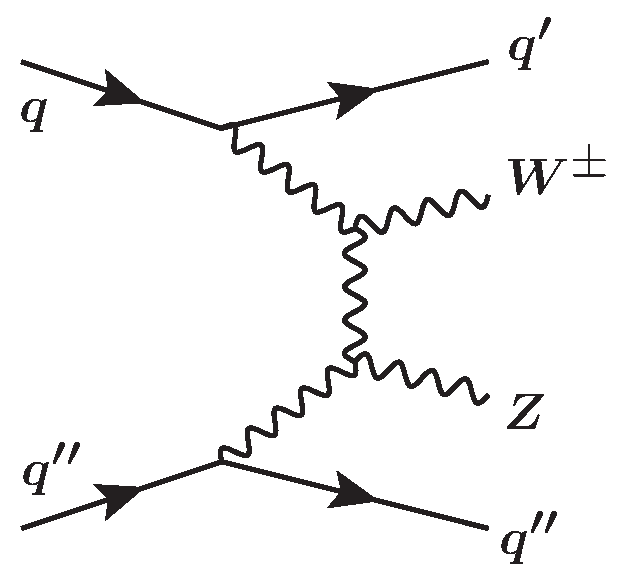
\includegraphics[width=0.22\textwidth]{Immagini/fig_01a.pdf} 
\hspace*{0.2cm}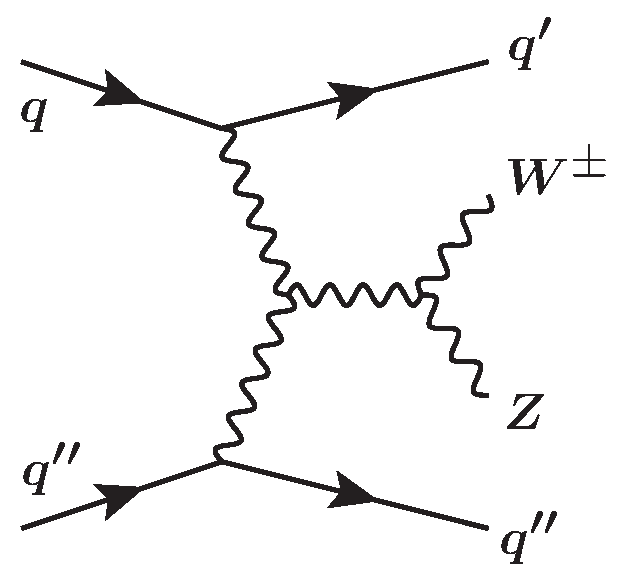
\includegraphics[width=0.22\textwidth]{Immagini/fig_01b.pdf} 
\hspace*{0.2cm}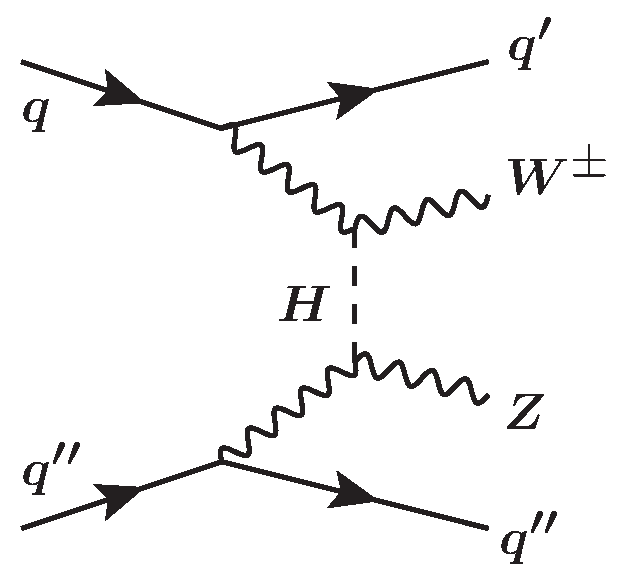
\includegraphics[width=0.22\textwidth]{Immagini/fig_01c.pdf} 
\hspace*{0.2cm}\hspace*{0.2cm}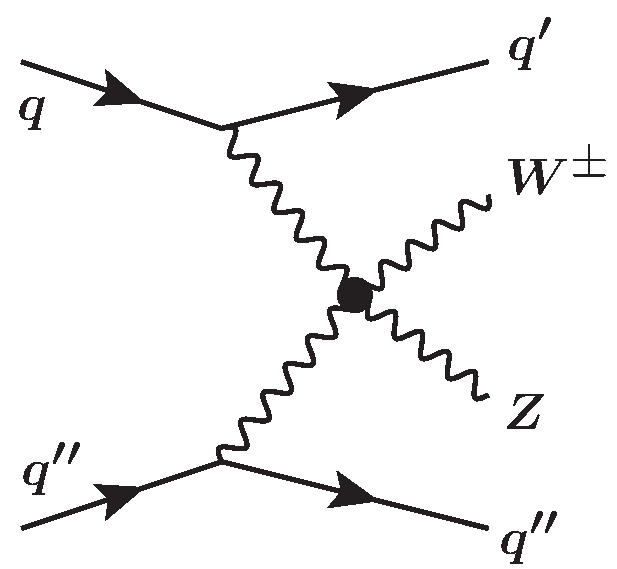
\includegraphics[width=0.22\textwidth]{Immagini/fig_01d.pdf} 
\caption{Diagrammi rappresentativi al LO della produzione \wzjjew in collisione $pp$.}
\label{fig:diag_WZjjEW}
\end{center}
\end{figure}
 
 
 
\begin{figure}[t]
\begin{center}
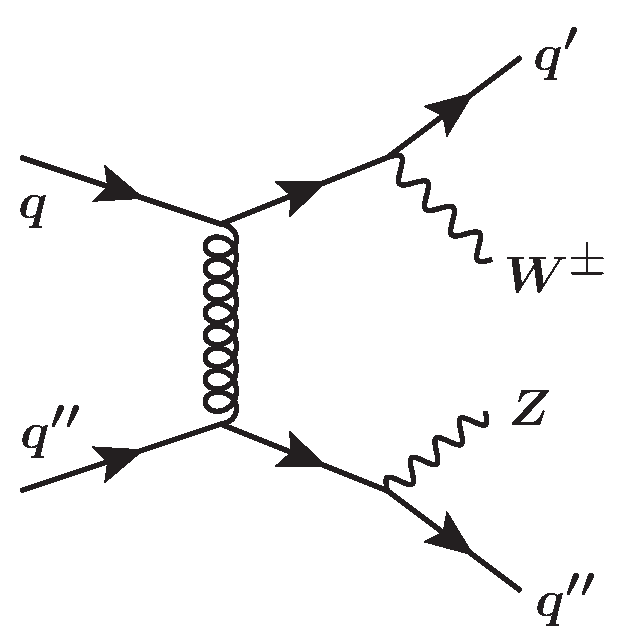
\includegraphics[width=0.22\textwidth]{Immagini/fig_02a.pdf} 
\hspace*{0.2cm}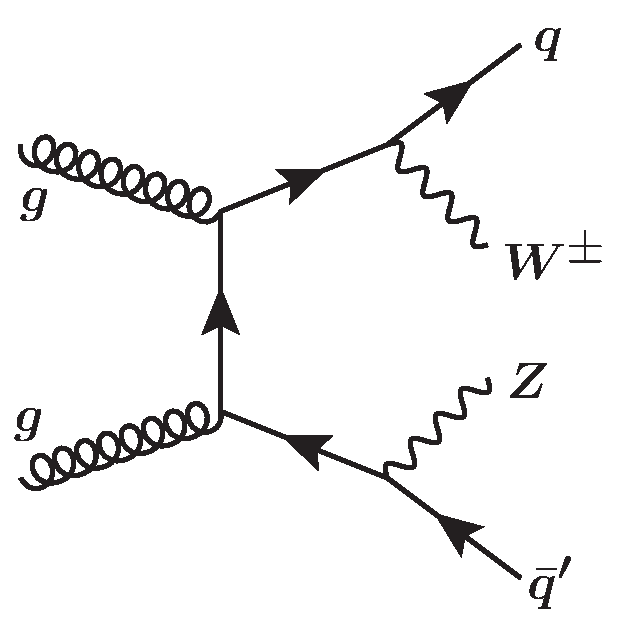
\includegraphics[width=0.22\textwidth]{Immagini/fig_02b.pdf} 
\hspace*{0.2cm}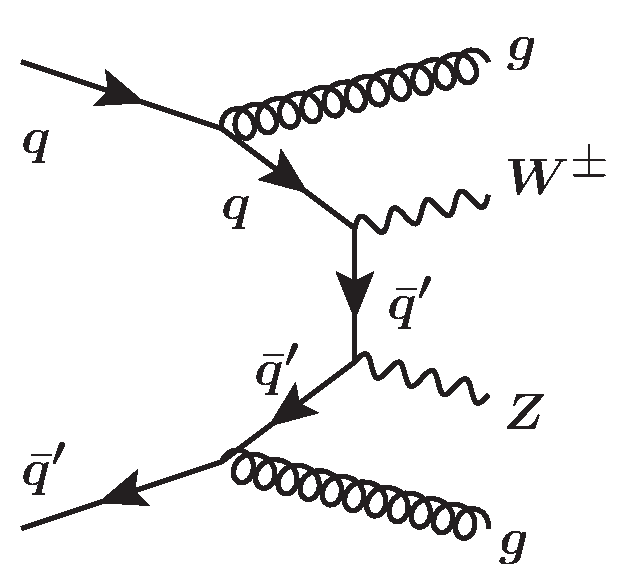
\includegraphics[width=0.22\textwidth]{Immagini/fig_02c.pdf} 
\caption{Diagrammi rappresentativi al LO della produzione \wzjjqcd in collisione $pp$.
}
\label{fig:diag_WZjjQCD}
\end{center}
\end{figure}
Questo articolo presenta le misure delle sezioni d'urto integrate e differenziali per la produzione elettrodebole e inclusiva di \wzjj, sfruttando i decadimenti completamente leptonici dei bosoni $Z$ e $W$ in cui i leptoni carichi nello stato finale sono elettroni o muoni. I dati delle collisioni $pp$ sono stati raccolti con il rivelatore ATLAS dal $2015$ al $2018$ a un'energia nel centro di massa di $\sqrt{s} = 13\,\unit{TeV}$ e corrispondono a una luminosità integrata di $140\,\unit{fb}^{-1}$. Un discriminante multivariato costruito a partire da un boosted decision tree (BDT) viene utilizzato per separare i modi di produzione elettrodebole e forte di \wzjj. Le loro rispettive sezioni d'urto sono misurate integrate su uno spazio delle fasi fiduciale. Sono inoltre misurate in modo differenziale in tre bin della massa invariante dei due jet di tagging, \mjj, e separatamente per eventi con esattamente due jet o con più di due jet. La sezione d'urto della produzione inclusiva di \wzjj è misurata anche in modo differenziale in funzione di varie osservabili cinematiche sensibili alla modellizzazione dei generatori di eventi Monte Carlo (MC) o a effetti di nuova fisica. Le distribuzioni della massa trasversa del sistema \wz, \mtwz, e dello score del BDT sono utilizzate in un'interpretazione EFT per porre dei limiti agli operatori di dimensione-$8$.

\section{Il rivelatore ATLAS}
L'esperimento ATLAS al Large Hadron Collider (LHC) è un rivelatore generale progettato per studiare una vasta gamma di fenomeni fisici nelle collisioni protone-protone. 

\begin{figure}[t]
\centerline{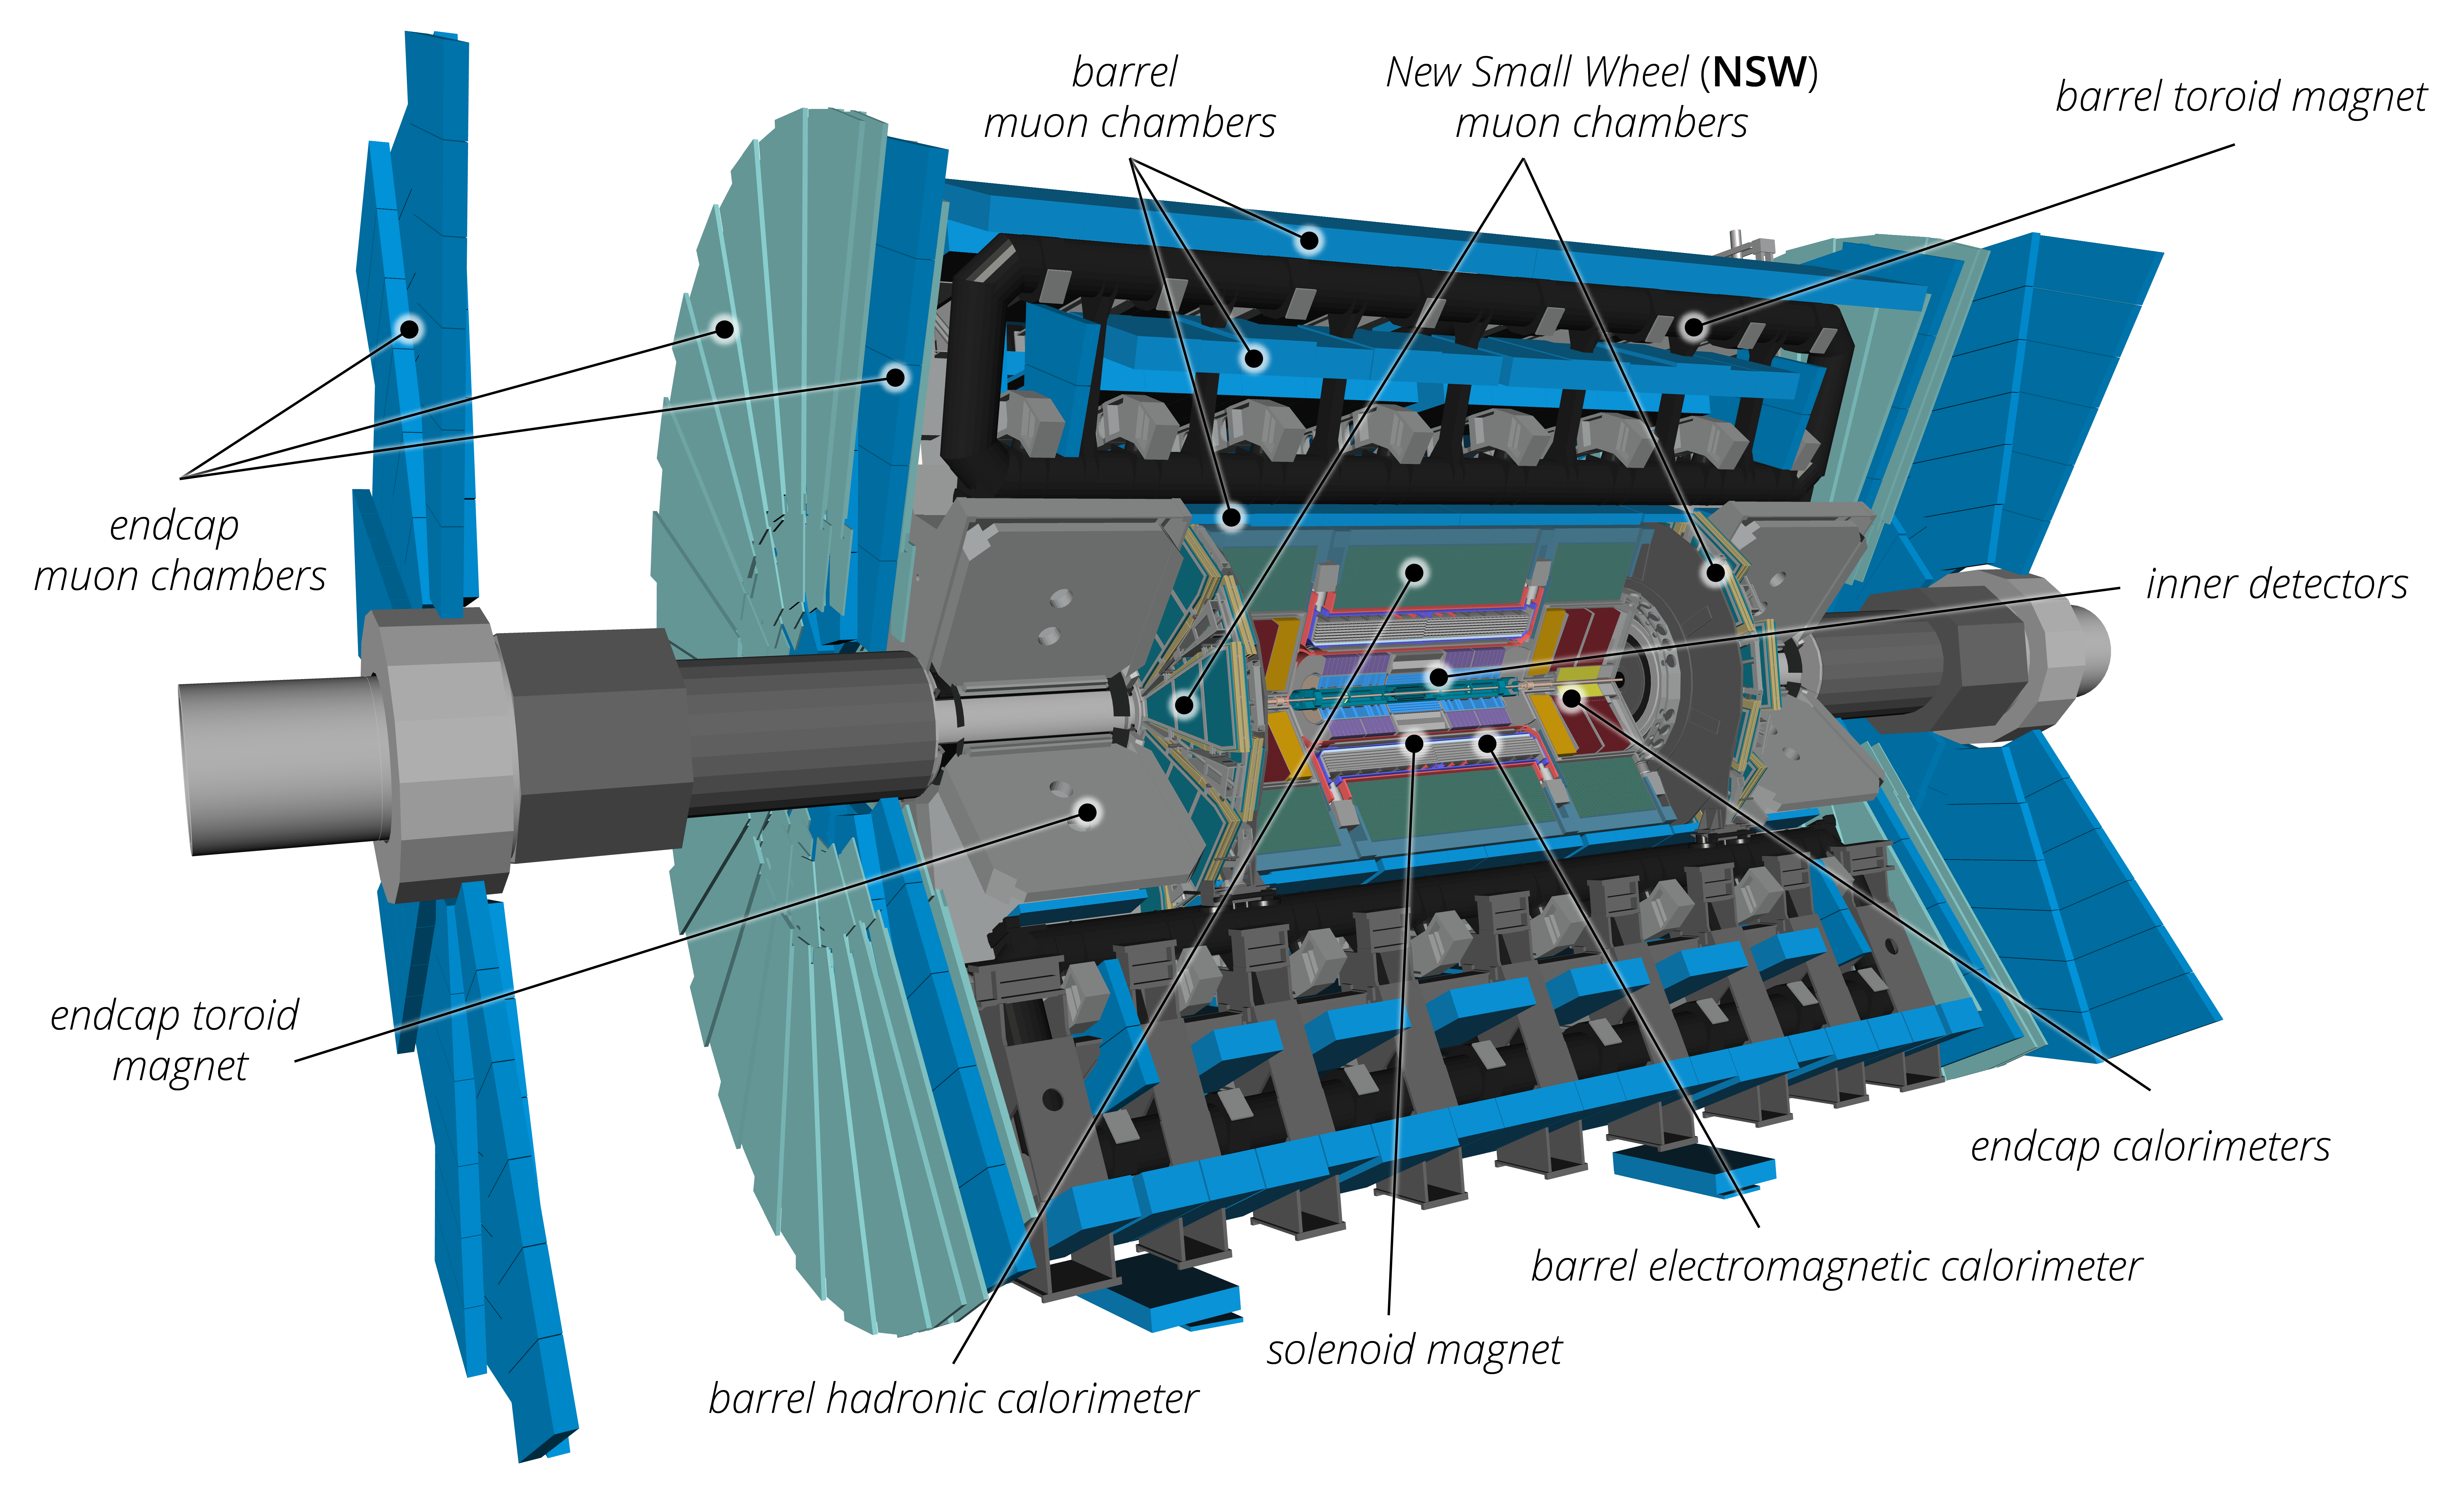
\includegraphics[width=0.95\textwidth]{Immagini/fig_02.png}}
\caption{Sezione trasversale del rivelatore ATLAS.}
\label{fig:Overview:ATLAS}
\end{figure}

Il rivelatore ATLAS all'LHC copre quasi l'intero angolo solido attorno al punto di collisione\footnote{ATLAS utilizza un sistema di coordinate destrorso con l'origine nel punto di interazione (IP) nominale al centro del rivelatore e l'asse $z$ lungo il tubo a vuoto (\textit{beam pipe}). L'asse $x$ punta dall'IP verso il centro dell'anello di LHC e l'asse $y$ punta verso l'alto. Nel piano trasverso vengono utilizzate le coordinate cilindriche $(r, \phi)$, dove $\phi$ è l'angolo azimutale attorno all'asse $z$. La pseudorapidità è definita in termini dell'angolo polare $\theta$ come $\eta = -\ln\tan(\theta/2)$. La distanza angolare è misurata in unità di $\Delta R \equiv \sqrt{(\Delta\eta)^2 + (\Delta\phi)^2}$.}. 
È costituito da un rivelatore di tracciamento interno circondato da un sottile solenoide superconduttore, calorimetri elettromagnetici e adronici, e uno spettrometro per muoni che incorpora tre grandi magneti toroidali superconduttori in aria. Le dimensioni del rivelatore sono $25\,\unit{m}$ di altezza e $44\,\unit{m}$ di lunghezza; il peso complessivo è di circa $7000\,\unit{t}$.

Il sistema del Tracciatore Interno (Inner Detector, ID) è immerso in un campo magnetico assiale di $2\,\unit{T}$ e fornisce il tracciamento delle particelle cariche nell'intervallo $|\eta| < 2.5$. Il rivelatore a Pixel in silicio ad alta granularità copre la regione del vertice e fornisce tipicamente quattro misure per traccia, con il primo \textit{hit} che cade normalmente nell'Insertable $B$-Layer (IBL) installato prima del Run 2 . Questo è seguito dal Semiconductor Tracker (SCT), un tracciatore a microstrip di silicio che fornisce solitamente otto misure per traccia. Questi rivelatori al silicio sono completati dal Transition Radiation Tracker (TRT), che consente una ricostruzione delle tracce estesa radialmente fino a $|\eta| = 2.0$. Il TRT fornisce inoltre informazioni per l'identificazione degli elettroni basate sulla frazione di hit al di sopra di una soglia più elevata di deposito di energia, corrispondente alla radiazione di transizione.

Il sistema calorimetrico copre l'intervallo di pseudorapidità $|\eta| < 4.9$. All'interno della regione $|\eta| < 3.2$, la calorimetria elettromagnetica è fornita da calorimetri a piombo/Argon Liquido (LAr) ad alta granularità suddivisi in \textit{barrel} (sezione centrale) ed \textit{endcap} (tappi), con un sottile \textit{presampler} aggiuntivo a LAr che copre la regione $|\eta| < 1.8$ per correggere la perdita di energia nel materiale a monte dei calorimetri. La calorimetria adronica è fornita dal calorimetro a tegole di acciaio/scintillatore (\textit{tile calorimeter}), segmentato in tre strutture \textit{barrel} entro l'intervallo $|\eta| < 1.7$, e da due calorimetri adronici \textit{endcap} in rame/LAr. La copertura dell'angolo solido è completata da moduli calorimetrici in avanti (\textit{forward}) in rame/LAr e tungsteno/LAr, ottimizzati rispettivamente per le misure di energia elettromagnetica e adronica.

Lo Spettrometro per Muoni (Muon Spectrometer, MS) comprende camere separate per il \textit{trigger} e per il tracciamento ad alta precisione, le quali misurano la deflessione dei muoni in un campo magnetico generato dai magneti toroidali superconduttori in aria. L'integrale di campo dei toroidi varia tra $2.0$ e $6.0\,\unit{T\cdot m}$ in gran parte del rivelatore.

Gli eventi interessanti vengono selezionati dal sistema di \textit{trigger} di primo livello (L1), implementato in hardware dedicato, seguito dalle selezioni effettuate tramite algoritmi implementati via software nell'\textit{high-level trigger} (HLT). Il \textit{trigger} di primo livello accetta eventi provenienti dagli incroci dei pacchetti (\textit{bunch crossings}) a $40\,\unit{MHz}$ con una frequenza inferiore a $100\,\unit{kHz}$, che il \textit{trigger} di alto livello riduce ulteriormente per registrare gli eventi su disco a circa $1\,\unit{kHz}$ (nella Run 3 si è alzato a $3\,\unit{kHz}$).

Un'estesa suite di software è utilizzata per la ricostruzione e l'analisi dei dati reali e simulati, per le operazioni del rivelatore e per i sistemi di \textit{trigger} e acquisizione dati dell'esperimento.

\section{Spazio delle fasi per la misura della sezione d'urto}
Le sezioni d'urto del processo $W^\pm Zjj$ vengono misurate all'interno di uno \textit{Spazio delle Fasi Fiduciale}, definito rigorosamente a livello di particella generata (\textit{Particle Level} o \textit{Truth Level}). Questa scelta svincola la definizione teorica della misura dagli effetti strumentali (quali l'accettanza geometrica, l'efficienza di ricostruzione e la risoluzione del rivelatore ATLAS), permettendo la successiva estrazione della sezione d'urto fisica differenziale tramite la procedura di \textit{Unfolding}.

La regione fiduciale è definita dalla cinematica dello stato finale dei leptoni carichi (elettroni e muoni) \textit{prompt}, ovvero associati direttamente al decadimento dei bosoni $W^\pm$ e $Z$. I leptoni prodotti dal decadimento di adroni o dal decadimento di leptoni $\tau$ (e dei loro discendenti) sono considerati fondo e scartati dalla definizione del segnale.

Poiché i leptoni carichi subiscono un irraggiamento colineare nel vuoto subito dopo il decadimento (QED \textit{Final-State Radiation}, FSR), l'utilizzo del loro quadri-impulso esatto renderebbe la sezione d'urto teorica fortemente dipendente dai dettagli del generatore Monte Carlo utilizzato. Per evitare questo bias, a livello \textit{Truth} la cinematica dei leptoni carichi viene ridefinita tramite una procedura algoritmica di \textit{Dressing} (vestizione). Nello specifico, i quadri-impulsi di tutti i fotoni generati che si trovano entro un cono di distanza angolare $\Delta R = 0.1$ attorno alla direzione del leptone vengono sommati vettorialmente al quadri-impulso del leptone stesso. 

Questa procedura restituisce i cosiddetti \textit{Dressed Leptons}, i quali mimano a livello teorico il raggruppamento energetico che l'algoritmo di ricostruzione opererà sui \textit{cluster} del calorimetro elettromagnetico a \textit{Detector Level}. Tutti i tagli cinematici che definiscono la regione fiduciale dell'analisi vengono imposti esclusivamente sulle variabili cinematiche di questi leptoni "vestiti".

Come ho già detto prima i leptoni e i neutrini che non originano da leptoni $\tau$ o adroni sono matchati al decadimento da bosoni $W^\pm$ e $Z$ usando un generatore MC chiamato \textit{ algoritmo resonant shape}. Questo algoritmo si basa sul valore di un estimatore che si esprime come il prodotto delle due line-shape nominali di Breit-Wigner dei bosoni $W^\pm$ e $Z$:
\begin{equation*}
    P = \left| \frac{1}{ m^2_{(\ell^+,\ell^-)} - \left(m_Z^{\textrm{PDG}}\right)^2 + \textrm{i} \; \Gamma_Z^{\textrm{PDG}} \; m_Z^{\textrm{PDG}} } \right|^2  \times \; \left| \frac{1}{ m^2_{(\ell',\nu_{\ell'})} - \left(m_W^{\textrm{PDG}}\right)^2 + \textrm{i} \; \Gamma_W^{\textrm{PDG}} \; m_W^{\textrm{PDG}} } \right|^2 
\end{equation*}
dove $m_Z^{\textrm{PDG}}$ ($m_W^{\textrm{PDG}}$) e $\Gamma_Z^{\textrm{PDG}}$ ($\Gamma_W^{\textrm{PDG}}$)  sono i valori medi di massa e della larghezza di decadimento dei bosoni $Z$ ($W$) dal PDG. L'input di questo estimatore è costituito da tutte le possibili combinazioni di leptoni carichi e neutrini che soddisfano i criteri di selezione del segnale. La combinazione che massimizza il valore di $P$ viene considerata come quella corretta per il match tra leptoni e bosoni.

Lo spazio delle fasi fiduciale è definito da una serie di requisiti cinematici sui leptoni carichi e sui jet a livello di particella generata. Questi requisiti sono progettati per massimizzare la sensibilità alla produzione elettrodebole di $W^\pm Zjj$ e per minimizzare le contaminazioni da processi di fondo, mantenendo al contempo un'ampia accettanza per il segnale. I criteri di selezione includono:
\begin{itemize}
    \item I leptoni carichi che derivano dal decadimento del bosone $Z$ devono avere un momento trasverso $p_T>15\,\unit{GeV}$.
    \item Il leptone carico che deriva dal decadimento del bosone $W$ deve avere un momento trasverso $p_T>20\,\unit{GeV}$.
    \item Tutti i leptoni carichi devono avere una pseudorapidità $|\eta| < 2.5$.
    \item La massa invariante dei due leptoni carichi associati al bosone $Z$ deve essere compresa in un range di $10\,\unit{GeV}$ attorno alla massa nominale del $Z$, ovvero $|m_{\ell^+ \ell^-} - m_Z^{\textrm{PDG}}| < 10\,\unit{GeV}$ dove $m_Z^{\textrm{PDG}}=91.1876\,\unit{GeV}$.
    \item La massa trasversa di $W$ definita come $m_T^W = \sqrt{2\cdot p_T^\ell \cdot p_T^{\nu} [1 - \cos\Delta\phi(l,\nu)]}$ dove $\Delta\phi$ deve essere maggiore di $30\,\unit{GeV}$, dove $p_T^\ell$ e $p_T^{\nu}$ sono i momenti trasversi del leptone carico e del neutrino associati al bosone $W$, e $\Delta\phi(l,\nu)$ è l'angolo tra il leptone e il neutrino nel piano trasverso.
    \item La distanza angolare tra il leptone carico dal decadimento di $W^\pm$ e ognuno dei leptoni carichi dal decadimento di $Z$ deve essere maggiore di $\Delta R > 0.3$.
    \item La distanza angolare tra i leptoni carichi del dacadimento di $Z$ deve essere maggiore di $\Delta R > 0.2$.
\end{itemize}
Ovviamente a queste richieste deve aggiungersi anche la richiesta di avere almeno due jet ricostruiti attraverso l'algoritmo anti-$k_t$ con il parametro $R=0.4$ con le seguenti caratteristiche:
\begin{itemize}
    \item I jet devono avere un momento trasverso $p_T > 40\,\unit{GeV}$.
    \item I jet devono avere una pseudorapidità $|\eta| < 4.5$.
    \item La distanza angolare tra ogni jet e ogni leptone carico deve essere maggiore di $\Delta R(j,l) > 0.3$.
    \item I due jet di tagging devono essere in regioni opposte del rivelatore, ovvero devono soddisfare la condizione $\eta_{j1} \cdot \eta_{j2} < 0$.
    \item La massa invariante dei due jet con il più alto momento trasverso (jet di tagging) deve essere maggiore di $\mjj > 500\,\unit{GeV}$ per aumentare la sensitività alla produzione elettrodebole di $W^\pm Zjj$.
    \item Vengono esclusi gli eventi che contengono un jet identificato come contenente un quark $b$ (b-jet) per ridurre la contaminazione da processi di fondo che coinvolgono il quark $b$, come la produzione singola di top associata a una $Z$ ($tZj$).
\end{itemize}
Un aspetto cruciale della definizione teorica del segnale riguarda il trattamento del quark bottom. A livello di elemento di matrice (\textit{Matrix Element}), gli \textit{hard processes} che presentano un quark $b$ nello stato iniziale o finale vengono rigorosamente esclusi dalla definizione del segnale $WZjj$-EW. Un esempio emblematico è la produzione singola di top associata a una $Z$ ($tZj$), la quale avviene prevalentemente tramite lo scambio in canale-$t$ di un bosone $W$ tra un quark $b$ e un quark leggero. Tali diagrammi, essendo dominati dalla fisica del quark top, non contengono i vertici di auto-accoppiamento dei bosoni di gauge (TGC e QGC). 

Poiché l'obiettivo cardine della misura del Vector Boson Scattering è sondare il settore di rottura della simmetria elettrodebole e cercare eventuali anomalie nei vertici quartici, i processi legati al quark $b$ non trasportano l'informazione fisica d'interesse. Essi costituiscono unicamente un fondo irriducibile, che viene soppresso a livello sperimentale (\textit{Detector Level}) imponendo un rigoroso $b$-veto nella \textit{Signal Region}

Un riassunto completo di tutti i tagli cinematici che definiscono il volume fiduciale è riportato nella Tabella~\ref{tab:fiducial_phase_space}.
\begin{table}[htbp]
\centering
\renewcommand{\arraystretch}{1.4} % Aumenta leggermente lo spazio verticale tra le righe per maggiore leggibilità
\begin{tabular}{llc}
\hline
\textbf{Categoria} & \textbf{Variabile cinematica} & \textbf{Requisito} \\
\hline
\multicolumn{3}{c}{\textbf{Selezione dei Leptoni}} \\
\hline
Leptoni da $Z$ & Momento trasverso ($p_T^{\ell_Z}$) & $> 15\,\unit{GeV}$ \\
Leptone da $W$ & Momento trasverso ($p_T^{\ell_W}$) & $> 20\,\unit{GeV}$ \\
Tutti i leptoni & Pseudorapidità ($|\eta_\ell|$) & $< 2.5$ \\
Bosone $Z$ & Finestra di massa invariante ($|m_{\ell^+ \ell^-} - m_Z^{\textrm{PDG}}|$) & $< 10\,\unit{GeV}$ \\
Bosone $W$ & Massa trasversa ($m_T^W$) & $> 30\,\unit{GeV}$ \\
Isolamento angolare & Distanza tra leptoni da $Z$ ($\Delta R(\ell_{Z1}, \ell_{Z2})$) & $> 0.2$ \\
Isolamento angolare & Distanza tra leptone $W$ e leptoni $Z$ ($\Delta R(\ell_W, \ell_Z)$) & $> 0.3$ \\
\hline
\multicolumn{3}{c}{\textbf{Selezione dei Jet (algoritmo anti-$k_t$, $R=0.4$)}} \\
\hline
Tutti i jet & Momento trasverso ($p_T^j$) & $> 40\,\unit{GeV}$ \\
Tutti i jet & Pseudorapidità ($|\eta_j|$) & $< 4.5$ \\
Isolamento angolare & Distanza tra jet e leptoni ($\Delta R(j, \ell)$) & $> 0.3$ \\
Jet di tagging & Emisferi opposti ($\eta_{j1} \cdot \eta_{j2}$) & $< 0$ \\
Jet di tagging & Massa invariante ($m_{jj}$) & $> 500\,\unit{GeV}$ \\
\hline
\multicolumn{3}{c}{\textbf{Veto sui jet}} \\
\hline
Jet da quark $b$ & Assenza di $b$-jet nello stato iniziale/finale & $N_{b\text{-jet}} = 0$ \\
\hline
\end{tabular}
\caption{Riassunto dei requisiti cinematici che definiscono lo spazio delle fasi fiduciale per l'analisi della produzione di $W^\pm Zjj$.}
\label{tab:fiducial_phase_space}
\end{table}

\section{Simulazione Monte Carlo e Modellizzazione}

Per interpretare correttamente i dati raccolti dal rivelatore, è essenziale avere una simulazione accurata sia del processo di segnale che dei vari processi di fondo. Nell'analisi della produzione di \wzjj, la strategia di simulazione si articola in tre fasi principali: la generazione del segnale, la valutazione dei fondi e la simulazione del rivelatore.
%magari per i fondi potrei capire meglio come avviene la produzione e mettere in backup i diagrammi se dovesse chiedermeli
\subsection{Generazione del Segnale e Interferenza}
La simulazione degli eventi \wzjj\ è stata affidata principalmente al generatore \textsc{MadGraph5\_aMC@NLO}, interfacciato con \textsc{Pythia} per ricreare la cascata partonica (\textit{parton shower}) e l'adronizzazione. Le funzioni di distribuzione dei partoni (PDF) necessarie per descrivere la cinematica interna dei protoni collidenti sono state modellate utilizzando i set della collaborazione \textsc{NNPDF}. 

Poiché lo stato finale $VVjj$ può essere prodotto attraverso diverse interazioni, la simulazione è stata suddivisa in componenti distinte:
\begin{itemize}
    \item \textbf{Produzione elettrodebole (\wzjjew):} Rappresenta il vero e proprio segnale dell'analisi (che include il \textit{Vector Boson Scattering}). Viene calcolata a livello albero (LO) considerando processi puramente elettrodeboli (ordine $\alpha_{\mathrm{EW}}^6$). In questa fase, vengono generati due jet aggiuntivi da vertici elettrodeboli e si applica un veto categorico sui quark $b$.
    \item \textbf{Produzione forte (\wzjjqcd):} Considerata un fondo per l'analisi VBS, include i diagrammi dominati dall'interazione forte (ordine $\alpha_{\mathrm{EW}}^4$). Per avere una maggiore precisione, questa componente è calcolata al NLO in QCD e ammette la presenza di quark $b$.
    \item \textbf{Interferenza (\wzjj-INT):} Quantifica l'interferenza quantistica tra la produzione EW e quella QCD (ordine $\alpha_{\mathrm{s}}$). Calcolata al LO, si è scoperto che fornisce un contributo positivo: aumenta la sezione d'urto del segnale elettrodebole di circa il $6\%$ nella regione fiduciale, raggiungendo picchi del $12\%$ per eventi con tre o più jet ad alto momento trasverso ($p_T > 25\,\unit{GeV}$).
\end{itemize}
Per assicurarsi che i risultati non dipendano artificialmente dal software scelto, i fisici di ATLAS hanno generato campioni alternativi utilizzando i generatori \textsc{Sherpa} e \textsc{Herwig}. Il confronto tra questi generatori permette di stimare in modo rigoroso l'incertezza sistematica legata alla modellizzazione teorica.

\subsection{Modellizzazione dei Fondi}
Oltre alla produzione \wzjjqcd, esistono numerosi altri processi del Modello Standard che possono imitare il segnale nel rivelatore. Questi fondi si dividono in due categorie basate su come vengono stimati:
\begin{itemize}
    \item \textbf{Fondi con leptoni \textit{prompt} (veri):} Processi come la produzione di coppie $ZZ$, $WW$, tribosoni ($VVV$) o quark top associati a bosoni vettoriali ($t\bar{t}V$, $tZj$). Poiché producono leptoni reali ben definiti, il loro contributo è valutato interamente tramite simulazioni Monte Carlo (utilizzando generatori come \textsc{Sherpa} e \textsc{MadGraph}). In particolare, per il dominante fondo $ZZ$, è stata inclusa sia la produzione originata da coppie quark-antiquark ($q\bar{q}$) sia quella dominata dalla fusione di gluoni ($gg$).
    \item \textbf{Fondi con leptoni \textit{fake} (falsi):} Eventi in cui un jet adronico viene erroneamente identificato come un leptone dal rivelatore. Essendo un artefatto strumentale complesso da simulare, questo fondo viene valutato direttamente utilizzando tecniche guidate dai dati reali (\textit{data-driven}).
\end{itemize}

\subsection{Simulazione del Rivelatore e Correzioni}
Una volta generata la cinematica delle particelle, gli eventi Monte Carlo vengono passati attraverso \textsc{Geant4}, un software che simula fedelmente l'interazione delle particelle con la materia e l'elettronica del rivelatore ATLAS. 
Per replicare l'ambiente caotico di LHC, alla simulazione vengono sovrapposti eventi di \textit{pile-up} (collisioni protone-protone secondarie nello stesso incrocio di pacchetti). Infine, per garantire un accordo perfetto tra dati simulati e dati reali, vengono applicati dei fattori di correzione (\textit{scale factors}) al Monte Carlo, aggiustando la scala degli impulsi e le efficienze di tracciamento e isolamento per rispecchiare esattamente le prestazioni osservate del rivelatore durante la presa dati.

\begin{table}[htbp]
\centering
\renewcommand{\arraystretch}{1.4}
\begin{tabular}{p{3.2cm} p{3.2cm} p{5.2cm} p{2.5cm}}
\hline
\textbf{Categoria} & \textbf{Processi Principali} & \textbf{Origine / Descrizione} & \textbf{Metodo di stima} \\
\hline
\multicolumn{4}{c}{\textbf{Fondi Irriducibili (Leptoni reali / \textit{Prompt})}} \\
\hline
Produzione Forte & \wzjjqcd & Produce l'esatto stato finale del segnale, ma tramite l'interazione forte (QCD). & Monte Carlo \\
Bosoni Multipli & $ZZ$, $WW$, $VVV$ & Decadono in leptoni reali. Ad esempio $ZZ \to 4\ell$, dove un leptone non viene ricostruito o esce dall'accettanza. & Monte Carlo \\
Quark Top & $t\bar{t}V$, $tZj$ & Decadono producendo leptoni reali. Contaminano il segnale se il veto sui jet $b$ fallisce. & Monte Carlo \\
\hline
\multicolumn{4}{c}{\textbf{Fondi Riducibili (Leptoni falsi / \textit{Fake})}} \\
\hline
Jet misidentificati & $Z+$jet, $Z\gamma$, single top, $t\bar{t}$ & Un jet adronico, un fotone o un leptone non isolato viene erroneamente ricostruito dal rivelatore come un leptone \textit{prompt}. & \textit{Data-driven} \\
\hline
\end{tabular}
\caption{Classificazione dei processi di fondo in irriducibili (fisici) e riducibili (strumentali) per l'analisi della produzione di $W^\pm Zjj$.}
\label{tab:background_classification}
\end{table}
\section{Selezione degli eventi}
Sono stati registrati solo i dati con fasci stabili e con tutti i sottosistemi del rivelatore operativi. Gli eventi sono stati selezionati utilizzando un sistema di \textit{trigger} a più livelli con diverse soglie di momento trasverso e criteri di isolamento che dipende da periodo di run e dalla luminosità istantanea. L'efficienza combinata di questi trigger è del $99\%$ per \wzjj che soddisfano i criteri di selezione. Gli eventi devono avere un vertice primario compatibile con la luminosità nominale di LHC all'interno del detector di ATLAS. Il vertice primario è definito come il vertice con una traccia di almeno due particelle cariche che hanno come somma scalare dei momenti trasversi maggiore.
%ELETTRONI E MUONI
I candidati muoni sono identificati dalla traccia ricostruita nel Muon Spectrometer (MS) che è matchata a una traccia nel Tracciatore Interno (ID). La selezione di questi muoni è del tipo "medium". L'efficienza di questa selezione in $p_T$ e $\eta$ è del $98\%$. Il momento dei muoni è misurato combinando le misure del MS corrette con l'energia depositata nel calorimetro e insieme alle misure del ID. Il $p_T$ dei muoni deve essere $p_T>15\,\unit{GeV}$ e la sua pseudorapidità deve soddisfare $|\eta|<2.5$.

I candidati elettroni sono ricostruiti dai cluster di energia nel calorimetro elettromagnetico matchando con le tracce dell'ID. Gli elettroni sono identificati usando come discriminante una funzione di likelihood costruita con le informazioni per quanto riguarda la forma della shower elettromagnetica nel calorimetro, dalle proprietà delle traccie e dalla qualità del matching tra cluster e traccia. Gli elettroni devono soddisfare requisiti della funzione di likelihood di tipo "medium" che produce un'efficienza di identificazione totale del $90\%$. Il momento trasverso degli elettroni deve essere $p_T>15\,\unit{GeV}$ e la pseudorapidità deve soddisfare $|\eta|<1.37$ o $1.52<|\eta|<2.47$. Questa differenza con i muoni è presto spiegata. Per misurare l'energia di un elettrone, dobbiamo arrestarlo completamente. L'elettrone, essendo molto leggere e altamente relativistico, quando attraversa un materiale denso perde energia prevelantemente per radiazione di frenamento (bremsstrahlung), innescando a sua volta produzione di coppie $e^+e^-$, generando uno sciame elettromagnetico. ATLAS misura l'energia degli elettroni raccogliendo tutto questo sciame nel calorimetro elettromagnetico a Piombo/Argon Liquido. Il muone, al contrario, ha una massa circa 200 volte superiore. Alle energie di LHC il muone è una MIP. La sua perdita di energia per brem è soppressa quindi attraversa i calorimetri perdendo solo pochissima energia per eccitazione e ionizzazione. Il calorimetro elettromagnetico di ATLAS non è un blocco unico. Per ovvie ragioni cotruttive, è diviso in un Barrel (il barile centrale) e in due Endcaps (tappi laterali). La regione di transizione spaziale tra il barrel e l'endcap si trova esattamente nell'intervallo di pseudorapidità $1.37<|\eta|<1.52$ (definita in gergo crack region) in cui c'è una quantità massiccia di materia morta. 

Si richiede che i candidati elettroni e muoni provengano dal vertice primario. Pertanto, la significanza del parametro di impatto trasverso della traccia, calcolato rispetto alla linea del fascio, $|d_0/\sigma_{d_0}|$, deve essere minore di $3.0$ per i muoni e minore di $5.0$ per gli elettroni. Inoltre, si richiede che il parametro di impatto longitudinale, $z_0$ (definito come la differenza tra il valore di $z$ del punto sulla traccia in cui viene valutato $d_0$ e la posizione longitudinale del vertice primario), soddisfi la condizione $|z_0 \sin\theta| < 0.5\,\unit{mm}$. Ricordo che la $d_0$ è la distanza di minimo approccio e cioè la distanza della traccia estrapolata rispetto alla linde del fascio nel piano trasverso. Mentre la $z_0$ è la distanza calcolata sull'asse longitudinale z. Ma allora perchè è moltiplicata per $\sin\theta$? Perchè se un leptone viaggia molto in avanti (piccolo angolo polare $\theta$), un piccolo errore trasversale si traduce in un errore longitudinale $z_0$ gigantesco per pura proiezione geometrica. Moltiplicando per quel seno proiettiamo la distanza longitudinale in modo perpendicolare alla traccia, ottenendo la vera e propria distanza fisica tridimensionale minima dal vertice. 

Inoltre gli elettroni e i muoni hanno la necessità di essere isolati da altre particelle usando contemporaneamente informazione del cluster calorimetrico e informazioni di traccia dell'ID. Le richieste di isolamento per gli elettroni sono tunate per avere una efficienza di almeno $89\%$ per il $p_T>15\,\unit{GeV}$ e almento al $99\%$ per gli elettroni di $p_T>60\,\unit{GeV}$ mentre per i muoni per avere una efficienza di almeno $90\%$ per il $p_T>15\,\unit{GeV}$ e almento al $99\%$ per i muoni con $p_T>60\,\unit{GeV}$.
%JET
I jet adronici sono ricostruiti usando un algoritmo di \textit{particle-flow} basato su cluster topologici a energia positiva con soppressione del rumore nei calorimetri. L'energia depositata nei calorimetri dalle particelle cariche viene sottratta e sostituita dai momenti delle tracce associate a tali cluster topologici. Le tracce che non corrispondono al vertice primario non vengono utilizzate nella ricostruzione dei jet, eliminando in modo efficace il contributo del \textit{pile-up} da particelle cariche. 

I jet sono raggruppati tramite l'algoritmo anti-$k_t$ con un parametro di raggio $R = 0.4$. Essi sono calibrati in base alle misurazioni \textit{in situ} della scala di energia dei jet. Tutti i jet devono avere $p_T > 25\,\unit{GeV}$ ed essere ricostruiti nell'intervallo di pseudorapidità $|\eta| < 4.5$. 

Per ridurre l'impatto dei jet originati dalle interazioni di \textit{pile-up}, ai jet con $|\eta| < 2.4$ e $p_T < 60\,\unit{GeV}$, o con $2.5 < |\eta| < 4.5$ e $p_T < 120\,\unit{GeV}$, è richiesto di soddisfare rispettivamente i \textit{working point} tight e loose degli algoritmi di \textit{tagging} associati al vertice del jet e al vertice del jet in avanti (\textit{forward jet vertex}). 

I jet con $|\eta| < 2.5$ contenenti un adrone $b$ sono identificati tramite una rete neurale (NN) basata su \textit{deep-learning}, la quale sfrutta le caratteristiche distintive dei decadimenti degli adroni $b$ in termini di parametri di impatto delle tracce e vertici spostati (\textit{displaced vertices}) ricostruiti nel tracciatore interno. I jet originati da quark $b$ vengono selezionati impostando la soglia di output dell'algoritmo in modo da ottenere un'efficienza di selezione dei $b$-jet del $70\%$ in eventi $t\bar{t}$ simulati, con un fattore di reiezione di $40$ contro i jet da sapore leggero (\textit{light-flavour}). Le correzioni alle efficienze di \textit{flavour-tagging} si basano su analisi di calibrazione \textit{data-driven}.

%NEUTRINI
Il momento trasverso dei neutrini è stimato attraverso il missing trasverse momentum nell'eventi e quindi $E_T^\text{miss}$ che è calcolato come il vettore negativo somma dei momenti trasversi di tutte gli oggetti fisici hard aggiungendo anche un termine addizionale soft. IL termine soft è calcolato matchando il track dell'ID con il vertice primare e non assegnato ad altri oggetti hard.

%eventi generali
Gli eventi devono contenere esattamente $3$ leptoni candidati che soddisfano le richieste fatte sopra. Per assicurarci che l'efficienza di trigger è ben determinata almeno uno di questi candidati leptoni deve avere un $p_T>25\,\unit{GeV}$ per i dati del $2015$ e un $p_T>27\,\unit{GeV}$ per i dati dal $2016-2018$. Questa richiesta a livello del detector non è presente nella definizione dello spazio delle fasi fiduciale in quanto ridurrebbe questo spazio fiduciale di solo $0.02\,\unit{GeV}$.

%Background
Per sopprimere i processi di fondo con almeno quattro leptoni \textit{prompt}, gli eventi con un quarto candidato leptone che soddisfa criteri di selezione più loose vengono scartati. Per questa selezione più loose, il requisito sul $p_T$ del leptone è abbassato a $p_T > 5\,\unit{GeV}$, agli elettroni è permesso di essere ricostruiti nella regione $1.37 < |\eta| < 1.52$ e vengono utilizzati requisiti di identificazione \textit{loose} sia per gli elettroni che per i muoni. Un requisito meno stringente viene applicato per l'isolamento degli elettroni ed è basato esclusivamente sulle informazioni delle tracce del rivelatore interno (ID). Nessun algoritmo di identificazione dedicato viene utilizzato per sopprimere gli eventi con elettroni e muoni originati dal decadimento di leptoni $\tau$.

%si ritorna sui leptoni
Si richiede che gli eventi candidati presentino almeno una coppia di leptoni con lo stesso sapore e carica opposta, aventi una massa invariante compatibile con $m_Z^{\mathrm{PDG}}$ entro $10\,\unit{GeV}$. Questa coppia è considerata il candidato bosone $Z$. Se è possibile formare più di una coppia, viene scelta come candidato bosone $Z$ quella la cui massa invariante è più vicina a $m_Z^{\mathrm{PDG}}$. Il restante terzo leptone viene assegnato al decadimento del bosone $W$. Si richiede che la massa trasversa del candidato $W$, calcolata utilizzando l'energia trasversa mancante $E_{\mathrm{T}}^{\mathrm{miss}}$ e il $p_T$ del leptone associato, sia maggiore di $30\,\unit{GeV}$.

%fondo riducibile
I fondi originati da leptoni misidentificati vengono soppressi richiedendo che il leptone associato al bosone $W$ soddisfi criteri di selezione più stringenti. Il momento trasverso di questo leptone deve quindi essere maggiore di $20\,\unit{GeV}$. Questo leptone deve inoltre soddisfare i requisiti di identificazione e isolamento \textit{tight}, il che si traduce in un'efficienza compresa tra il $90\%$ e il $98\%$ a seconda del $p_T$ per i muoni, e in un'efficienza complessiva dell'85\% per gli elettroni.

Per selezionare i candidati $W^\pm Zjj$, si richiede ulteriormente che agli eventi siano associati almeno due jet di \textit{tagging}. Il jet di \textit{tagging} principale (\textit{leading}) viene scelto come il jet con il $p_T$ più alto nell'evento, con $p_T > 40\,\unit{GeV}$. Il secondo jet di \textit{tagging} è selezionato come quello con il $p_T$ più alto tra i restanti jet che hanno una pseudorapidità di segno opposto rispetto al primo jet di \textit{tagging} e un $p_T > 40\,\unit{GeV}$. Si richiede infine che questi due jet soddisfino $m_{jj} > 150\,\unit{GeV}$, al fine di minimizzare la contaminazione da processi con tribosoni.

La regione di segnale finale (SR) per il VBS è definita richiedendo che la massa invariante dei due tagging jets \mjj sia maggiore di $500\,\unit{GeV}$ e che non ci siano $b-$jet nell'evento.

\begin{table}[htbp]
\centering
\renewcommand{\arraystretch}{1.4}
\begin{tabular}{p{4.5cm} p{10cm}}
\hline
\textbf{Categoria} & \textbf{Criteri di Selezione} \\
\hline
\multicolumn{2}{c}{\textbf{Selezione degli Oggetti Fisici}} \\
\hline
\textbf{Muoni} & Identificazione \textit{Medium} (MS + ID) \newline
$p_T > 15\,\unit{GeV}$, $|\eta| < 2.5$ \newline
Parametri d'impatto: $|d_0/\sigma_{d_0}| < 3.0$, $|z_0 \sin\theta| < 0.5\,\unit{mm}$ \newline
Isolamento: Efficienza $90-99\%$ a seconda del $p_T$ \\
\hline
\textbf{Elettroni} & Identificazione \textit{Medium} (Likelihood) \newline
$p_T > 15\,\unit{GeV}$, $|\eta| < 1.37$ oppure $1.52 < |\eta| < 2.47$ (esclusione \textit{crack region}) \newline
Parametri d'impatto: $|d_0/\sigma_{d_0}| < 5.0$, $|z_0 \sin\theta| < 0.5\,\unit{mm}$ \newline
Isolamento: Efficienza $89-99\%$ a seconda del $p_T$ \\
\hline
\textbf{Jet (anti-$k_t$, $R=0.4$)} & $p_T > 25\,\unit{GeV}$, $|\eta| < 4.5$ \newline
Veto \textit{pile-up}: JVT \textit{tight} ($p_T < 60\,\unit{GeV}, |\eta| < 2.4$) e fJVT \textit{loose} ($p_T < 120\,\unit{GeV}, 2.5 < |\eta| < 4.5$) \\
\hline
\textbf{Neutrini} & Stima basata su $E_{\mathrm{T}}^{\mathrm{miss}}$ (somma vettoriale degli oggetti fisici \textit{hard} + termine \textit{soft}) \\
\hline
\multicolumn{2}{c}{\textbf{Selezione dell'Evento (Topologia $W^\pm Z$)}} \\
\hline
\textbf{Selezione preliminare} & Esattamente 3 leptoni candidati ($\mu$ o $e$) \newline
Veto su un possibile $4^\circ$ leptone \textit{loose} ($p_T > 5\,\unit{GeV}$) \newline
Matching col trigger: almeno 1 leptone con $p_T > 25$ ($2015$) o $27\,\unit{GeV}$ ($2016-2018$) \\
\hline
\textbf{Candidato Bosone $Z$} & Coppia di leptoni stesso sapore e carica opposta (OSSF) \newline
$|m_{\ell\ell} - m_Z^{\mathrm{PDG}}| < 10\,\unit{GeV}$ (se ambiguità, si sceglie la massa più vicina a $m_Z$) \\
\hline
\textbf{Candidato Bosone $W$} & Il $3^\circ$ leptone (associato a $E_{\mathrm{T}}^{\mathrm{miss}}$) \newline
Requisiti più stringenti: ID e Iso \textit{tight}, $p_T > 20\,\unit{GeV}$ \newline
Massa trasversa: $m_T^W > 30\,\unit{GeV}$ \\
\hline
\multicolumn{2}{c}{\textbf{Regione di Segnale VBS (\wzjj SR)}} \\
\hline
\textbf{Jet di Tagging} & I due jet a $p_T$ maggiore (almeno $40\,\unit{GeV}$) \newline
Devono risiedere in emisferi opposti ($\eta_{j1} \cdot \eta_{j2} < 0$) \\
\hline
\textbf{Filtri Cinematici SR} & $m_{jj} > 150\,\unit{GeV}$ (taglio preliminare anti-tribosoni) \newline
$m_{jj} > 500\,\unit{GeV}$ (definizione finale per isolare il processo EW) \newline
Veto assoluto sui quark $b$ ($N_{b\text{-jet}} = 0$) \\
\hline
\end{tabular}
\caption{Riassunto dei criteri di selezione per la ricostruzione degli oggetti fisici e la definizione della regione di segnale per l'analisi $W^\pm Zjj$.}
\label{tab:event_selection}
\end{table}
\subsection{Jet e JADE}
Essendo LHC una macchina adronica la maggior parte degli oggett che vedremo saranno jet adronici! Ma prima ricostruiamo un attimo la nostra conoscenza dei Jet. I Jet in maniera naively sono un chunk di particelle collimate che derivano da una frammentazione dei partoni. Abbiamo bisogno di un modo per definire un processo per definire questi jet senza essere troppo sensibili per i sottoprocessi soft come ad esempio radiazione di gluone al NLO etc. Ovviamente non possiamo avere un perfetto match tra partone e jet qusto perchè i partoni sono colorati mentre i jet non lo sono. Partendo dall'algoritmo di JADE: idealmente raggruppiamo oggetti molto vicini nello spazio delle fasi che significa in soldoni che raggruppo oggetti con una piccola massa invariante. Ricordiamoci:
\begin{equation}
    m_{jk}^2=(E_j+E_k)^2-(\mathbf{p}_j+\mathbf{p}_k)^2\approx2E_jE_k(1-\cos\alpha_{jk})
\end{equation}
dove $\alpha_{jk}$ è l'angolo tra l'oggetto $j$ e $k$. Ora definiamo appunto la distanza in questo spazio delle fati come
\begin{equation}
    y_{jk}=\frac{m_{jk}^2}{Q^2}=\frac{2}{Q^2}E_jE_k(1-\cos\alpha_{jk}) \qquad \text{dove} \qquad Q=\left(\sum_jE_j\right)^2- \left(\sum_j\mathbf{p}_j\right)^2
\end{equation}
l'algoritmo è costituito nel seguente modo:
\begin{enumerate}
    \item inizio con una lista di oggetti ognuno con un quadrimomento $p_j\equiv(E_j;\mathbb{p}_j)$
    \item calcolo la distanza $y_{jk}$ tra tutte le coppie di oggetti $(jk)$
    \item scelgo la coppia con il valore di $y_{jk}$ più piccolo e se questo valore è minore di un $y_\text{cut}$ che scelgo io allora questi due oggetti si uniranno in un solo oggetto con quadrimomento $p_j+p_k$ e la lista diminuisce di un oggetto e ricomincio dal punto $1$
    \item se il più piccolo $y_{jk}>y_\text{cut}$ allora fermo l'iterazione e nella lista dovrei avere solo jet. 
\end{enumerate}
Ovviamente dipende molto dalla scelta del cut.

\subsection{Anti-kt}
L'idea di base è molto simile a quella di JADE e quella fatta a LEP. Si parte da oggetti di cui conosciamo il quadriimpulso che può essere attraverso i cluster calorimetrici grazie al quale misuriamo l'energia e il centroide. Oppure posso usare delle tracks cariche. Ma quale dei due metodi è meglio? Ora ATLAS usa una sorta di particle-flow in cui si uniscono i due metodi ma è molto complicato per evitare il double counting. Anche in questo caso si cerca di rendere la massa invariante piccola.
\begin{equation}
    m_{ij}^2 = 2p_{\mathrm{T}}^{(i)} p_{\mathrm{T}}^{(j)} \left[ \cosh(\eta^{(i)} - \eta^{(j)}) - \cos(\phi^{(i)} - \phi^{(j)}) \right] \simeq p_{\mathrm{T}}^{(i)} p_{\mathrm{T}}^{(j)} \left[ (\Delta\eta)^2 + (\Delta\phi)^2 \right]
\end{equation}
Questo è il punto di partenza. Ci sono però due argomenti che ci portano a modificare questo criterio ad LHC. Una formula di questo genere ha lo stesso problema dell'algoritmo di JADE e cioè che due oggetti lontani (grande $\Delta \eta$ e $\Delta \phi$) potrebbero essere raggruppati ugualmente se entrambi hanno un $p_T$ molto piccolo. Inoltre questa metrica è sensibile ovviamente agli oggetti soft. Ad LHC abbiamo sia il pile-up che gli underlying event che sono oggetti soft e meno interessanti.

C'è bisogno di una modifica della metrica da usare. L'idea è questa: abbiamo i nostri oggetti e chiamo $k_j$ l'impulso del j-esimo oggetto $k_j=(E_j;\mathbf{p}_j)$ e posso scomporlo in componenti: $k_T^{(j)}$, $Y^{(j)}$ e $\phi^{(j)}$. Da notare che usiamo la rapidità e non la pseudorapidità perchè i due oggetti coincidono quando la massa dell'oggetto è trascurabile. Quando parto con l'algoritmo la situazione è accettabile ma man mano che aumento gli oggetti uniti la massa dell'oggettone aumenta. Quello che facciamo quindi è definire la nostra distanza fra due oggetti. Quindi al posto di eta uso Y e normalizzo la quantità sommata per un parametro R fisso che mi dirà circa quanto largo verrà il nostro oggetto. Poi davanti al posto di fare il prodotto dei momenti traversi dei due oggetti vado a fare il minimo dei due momenti trasversi esponenziati per un certo p.
\begin{equation*}
    d_i = \left(k_T^{(i)}\right)^{2p} \quad ; \quad
    d_{ij} = \min \left[ \left(k_T^{(i)}\right)^{2p} ; \left(k_T^{(j)}\right)^{2p} \right] \frac{\overbrace{(\Delta Y)^2 + (\Delta\phi)^2}^{\equiv (\Delta R)^2}}{R^2}
\end{equation*}
\begin{center}
\begin{tabular}{l|r}
    nome & $p$ \\
    \hline
    $k_T$ & $1$ \\
    Cambridge-Aachen & $0$ \\
    anti-$k_T$ & $-1$
\end{tabular}
\end{center}
Se usiamo $p = 1$ stiamo praticamente facendo i quadrati dei momenti trasversi quando invece $p = 0$ non stiamo usando i momenti ma usiamo solo le distanze nel piano. Quando usiamo il $p = -1$ che è anche il metodo più usato qui stiamo facendo gli inversi dei quadrati. Quindi il minimo degli inversi sarà in realtà il massimo fra i due. Poi definisco la distanza di un solo oggetton $d_i$

\noindent L'algoritmo per i jet è iterativo:
\begin{enumerate}
    \setcounter{enumi}{-1}
    \item iniziare con una lista di ``oggetti'', definiti come gli oggetti elementari, ciascuno con quadrimpulso $k_j \equiv (E_j; \vec{p}_j)$
    \item calcolare $d_i$ per ogni oggetto $i$, e $d_{ij}$ per ogni coppia $(i,j)$, e il loro minimo $d_{\min} = \min(\{d_i\} \cup \{d_{ij}\})$
    \item se esiste un oggetto $i$ tale che $d_i \equiv d_{\min} \implies i$ è definito come un jet e rimosso dalla lista degli oggetti
    \item altrimenti deve esserci una coppia $(i,j)$ tale che $d_{ij} \equiv d_{\min} \implies$ raggruppare insieme gli oggetti $i,j$, per formare un nuovo oggetto con quadrimpulso $k_i + k_j$; inserire il nuovo oggetto nella lista degli oggetti e rimuovere gli oggetti $i,j$ dalla lista
    \item reiterare da (1) finché non ci sono più oggetti nella lista: rimaniamo con i jet!
\end{enumerate}

\noindent \textbf{Nota:} tutte le quantità sono invarianti di Lorentz per boost lungo l'asse del fascio $\implies$ il clustering dei jet è ben definito!\\
\textbf{Nota:} si usa la rapidità $Y$ invece della pseudo-rapidità $\eta$ --- i jet sono larghi, hanno una massa invariante considerevole $\implies$ non si può approssimare $Y \to \eta$\\
\textbf{Nota:} (specialmente per $p=1$) la sostituzione $k_T^{(i)} k_T^{(j)} \to \min \left[ \left(k_T^{(i)}\right)^2 ; \left(k_T^{(j)}\right)^2 \right]$ evita la ricombinazione di due oggetti soft molto distanti, preferendo soft+hard a $\Delta R$ minore
\begin{figure}[t]
\begin{center}
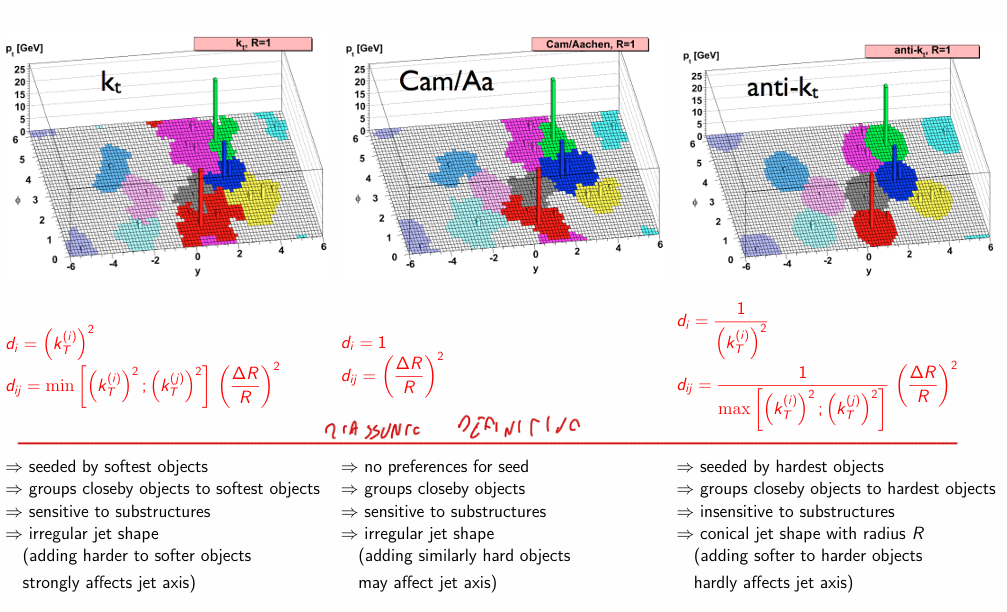
\includegraphics[width=1\textwidth]{Immagini/jet.png} 
\end{center}
\end{figure}

\section{Stima del Background}
Le sorgenti di background sono classificate in due gruppi:
\begin{itemize}
    \item \textbf{Fondo irriducibile}: eventi dove tutti i candidati sono leptoni prompt o sono prodotti da decadimenti del leptone $\tau$.
    \item \textbf{Fondo riducibile}: eventi dove almeno uno dei leptoni candidati non è di tipo prompt. Questi sono anche chiamati misidentified o fake lepton.
\end{itemize}
\subsection{Il background irriducibile}
Questo fondo deriva da $ZZ$ e $t\bar{t}V$ e sono modellizzati usando simulazioni Monte Carlo. I dati sono presi in due diverse control regions (CR) la prima riferita come $ZZ-CR$ e la seconda come $b-CR$ rispettivamente e sono usate per limitare la normalizzazione il fondo di $ZZjj$-QCD e $t\bar{t}V$. La regione di controllo $ZZ-CR$ è arricchita di eventi $ZZ$ ed è identificata applicando la selezione degli eventi \wzjj definiti nella sezione sopra ma al posto di vetare sul quarto leptone gli eventi devono avere almeno quattro leptoni candidati con una identificazione più looser. Ovviamente per costruzione questa regione è arricchita di eventi $ZZjj-$QCD con un piccolo contributo di $ZZjj-$EW. La regione di controllo $b-CR$ è arricchita di eventi $t\bar{t}V$ e $tZj$ ed è identificata applicando la selezione degli eventi \wzjj ma invece di vetare sui jet $b$ si richiede che ci siano almeno un jet $b$. Le sorgenti rimanentti di fondo irriducibile sono $ZZjj$-EW e $VVV$ e i loro contributi nella CR e SR sono valutati interamente tramite simulazione Monte Carlo.
\subsection{Il background riducibile}
Il fondo riducibile origina dalla produzione di $Z+j$, $Z\gamma$, $t\bar{t}$, $Wt$ e $WW$. Questi fondi sono stimati usanto un metodo basato dul data-driven in cui avviene un'inversione della matrice globale che contiene i coefficienti di efficienza di identificazione e di fake lepton come candidato loose o tight. I letponi candidati tight sono quelli che soddisfano i criteri di selezione più stringenti citati precedentemente nella sezione dedicata. I loose lepton invece sono quelli che non riscontrano il criterio di isolamento e identificazione del segnale ma soddista comunque criteri più looser. La probabilità di misidentificazione di un un leptone sono determinate usando sample di controllo dedicati ognuno arricchino in leptoni misidentificati da una specifica sorgente di fondo come da jet di sapore leggero o pesante e da fotoni convertiti. Le efficienze e le probabilità di misidentificazione sono determinate in funzione del $p_T$ e $\eta$ del leptone candidato e sono combinate con gli event rate nei saple dei dati \wzjj dove almeno uno dei tre leptoni candidati è loose. Poi risolveco un sistema di equazioni lineari il numero di eventi con almeno un leptone misidentificato è ottenuto e questo rappresenta il numero di di eventi di fondo riducibile nel \wzjj sample. Oltre a questo è stato anche utilizzato un secondo metodo indipendente basato su simulazione MC scalate sui dati da un fattore  process-dependet determinato da data-to-MC con un comparison nella CR. L'articolo afferma che è presente un agreement tra i due metodi entro il 20\%. Questo tipo di accordo è compatibile con le incertezze sistematiche. Nella seguente sabella è possibile gli eventi attesi da simulazioni MC e dal fondo stimato dal data-driven per il fondo riducibile.
\begin{table}[htbp] 
\centering
\renewcommand{\arraystretch}{1.4} % Aumenta lo spazio verticale per facilitare la lettura
\begin{tabular}{l c c c c}
\hline
\textbf{Processo} & \textbf{SR ($N_{\text{jet}} = 2$)} & \textbf{SR ($N_{\text{jet}} \ge 3$)} & \textbf{$b$-CR} & \textbf{$ZZ$-CR} \\
\hline
\hline
\textbf{Dati osservati} & 169 & 477 & 666 & 210 \\
\textbf{Totale atteso} & 231 $\pm$ 12 & 550 $\pm$ 50 & 660 $\pm$ 40 & 205 $\pm$ 11 \\
\hline
\wzjjew & 65.0 $\pm$ 3.5 & 60 $\pm$ 6 & 4.82 $\pm$ 0.28 & 0.725 $\pm$ 0.014 \\
\wzjjqcd & 125 $\pm$ 9 & 380 $\pm$ 50 & 77 $\pm$ 18 & 6.2 $\pm$ 0.7 \\
\wzjj-INT & 1.3 $\pm$ 0.6 & 5.3 $\pm$ 2.6 & 0.58 $\pm$ 0.29 & 0.22 $\pm$ 0.11 \\
$t\bar{t}+V$ & 0.66 $\pm$ 0.04 & 20.2 $\pm$ 0.7 & 289 $\pm$ 10 & 9.89 $\pm$ 0.28 \\
$tZj$ & 8.78 $\pm$ 0.34 & 19.7 $\pm$ 1.2 & 134 $\pm$ 4 & 0.432 $\pm$ 0.005 \\
$ZZ$-QCD & 9.6 $\pm$ 0.4 & 32.0 $\pm$ 2.5 & 10.1 $\pm$ 0.6 & 159 $\pm$ 9 \\
$ZZ$-EW & 2.2 $\pm$ 0.6 & 4.4 $\pm$ 1.1 & 0.25 $\pm$ 0.06 & 23 $\pm$ 6 \\
$VVV$ & 0.41 $\pm$ 0.10 & 2.0 $\pm$ 0.5 & 0.39 $\pm$ 0.10 & 4.1 $\pm$ 1.1 \\
Leptoni \textit{fake} & 18 $\pm$ 4 & 28 $\pm$ 7 & 150 $\pm$ 40 & 1.7 $\pm$ 0.5 \\
\hline
\end{tabular}
\caption{Numero di eventi attesi e osservati nella regione di segnale (SR) per la produzione di $W^\pm Zjj$ e nelle due regioni di controllo ($b$-CR e $ZZ$-CR), prima dell'esecuzione del fit globale. Sono mostrati i conteggi attesi per il segnale elettrodebole, la produzione forte e la loro interferenza, insieme alla stima degli eventi degli altri processi di fondo. La categoria ``Leptoni \textit{fake}'' raggruppa tutti i fondi riducibili. Le incertezze riportate rappresentano l'incertezza sistematica totale pre-fit.}
\label{tab:VBSyield_prefit}
\end{table}
Le varie incertezze saranno presentate nella sezione dedicata. Quindi il contributo atteso di \wzjjew nella SR \wzjj è di circa il $16\%$ mentre il $64\%$ dei dati sono attesi essere prodotti da \wzjjqcd. IL contribuoto di \wzjj con leptoni $\tau$ ammonta al $5.3\%$ di tutti gli eventi \wzjj dove sono inclusi \wzjjew, \wzjjqcd e \wzjj-INT.

\section{Metodologie di Misura}
\subsection{WZjj-EW e WZjj-QCD misura integrata}
Gli eventi associati alla produzione di \wzjjew sono reparati dagli altri eventi di \wzjj originati da \wzjjqcd e da \wzjj-INT basate dalle loro proprietà cineamtiche modellate da predizioni MC. La sezione d'urto di produzione dei due eventi $\sigma_{WZjj-EW}$ e $\sigma_{WZjj-QCD}$ sono misurate simultaneamente.

Dato il piccolo contributo della SR del processo \wzjjew è stata usata una discriminante multivariata  per separare il segnale dal backgrounds. Quindi un BDT è stato implementato nel pacchetto TMVA ed è usato per scovare le differenze cinematiche tra il segnale \wzjjew e \wzjjqcd e altri fondi di altri processi. Il BDT è allenato e ottimizzato su eventi simulati dalla SR per separare il segnale \wzjjew da \wzjjqcd e altri processi di fondo.

Sono state usate $15$ variabili cinematihe come input per il distriminate BDT. Le variabili possono essere classificate in tre categorie: variabili che descrivono i jet di tagging, variabili che descrivono il sistema $WZ$ e variabili che descrivono le relazioni cinematihe tra i jet di tagging e la cinematica dei leptoni. Le variabili per i due tagging jet sono la massa invariante $m_{jj}$, il momento traverso dei due jet $p_T^{j1}$ e $p_T^{j2}$, la differenza di pseudorapidità $\Delta \eta_{jj}$ e la differenza di azimuth $\Delta \phi_{jj}$. Le variabili che descrivono il sistema $WZ$ sono il momento trasverso dei due bosoni $p_T^W$ e $p_T^Z$, la pseudorapidità del bosone $W$ e la differenza assoluto tra le rapidità di $Z$ e dei leptoni che decadono dalla $W$ $|\Delta \eta_{Z,\ell_W}|$ e la massa trasversa del sistema $W^{\pm}Z$ $m_T^{WZ}$. La pseudorapidità del bosone $W$ è ricostruita stimando il momento longitudinale del neutrino ottenuto usando un metodo di neural-network. Le variabili che descrivono le relazioni cinematiche tra i jet di tagging e i leptoni sono la distanza nel piano pseudorapidità-azimutale tra il bosone Z e il jet leading $\Delta R_{Z,j1}$, il bilancio dell'evento $R_{pT}^{hard}$ definito come la componente trasversa del vettore somma dei $WZ$ e dei due jet di tagging normalizzato per la somma dei momenti trasversi dei $WZ$ e dei due jet di tagging e infine la centralità del sistema $WZ$ relativo ai due jet definita come: 
\begin{equation}
    \xi_\text{lep.}=\text{min}(\Delta\eta_-,\Delta\eta_+)
\end{equation}
con
\begin{equation}
    \Delta\eta_-=\text{min}(\eta_l^W, \eta_{l2}^Z,\eta_{l1}^Z)-\text{min}(\eta_{j1},\eta_{j2})\qquad \Delta\eta_+=\text{max}(\eta_{j1},\eta_{j2})-\text{max}(\eta_l^W, \eta_{l2}^Z,\eta_{l1}^Z)
\end{equation}
Per garantire che il BDT non impari artefatti introdotti dal Monte Carlo, l'analisi valida la cinematica degli eventi attraverso tre passaggi chiave: 
primo, controllando le distribuzioni in una \textit{Validation Region} adiacente al segnale ($150 < \mjj < 500\,\unit{GeV}$). 
Secondo, utilizzando una rete neurale "avversaria" (ANN) che permette di isolare un sotto-campione arricchito di fondo QCD direttamente nella \textit{Signal Region}, senza però alterare (scolpire) lo spettro della variabile \mjj. 
Terzo, verificando a posteriori che le sezioni d'urto differenziali misurate e corrette per gli effetti del rivelatore tramite \textit{unfolding} combacino con le previsioni teoriche al NLO.

Per separare il segnale $t\bar{t}V$ e $tZj$ nella $b-$CR e per limitare di entrambi i contributi usando i dati in questa CR un secondo BDT chiamato $b-$CR BDT è stato implementato usando $16$ variabili di input. Le variabili di input utilizzate nel BDT sono legate alla cinematica dei jet di \textit{tagging} ($p_T^{j1}, \eta_{j1}, \phi_{j1}, p_T^{j2}, \Delta\eta_{jj}$ e $\Delta\phi_{jj}$), alla cinematica dei bosoni vettoriali ($p_T^Z, \eta_Z, \phi_Z, p_T^W, m_{WZ}, \Delta\eta(W,Z)$ e $\Delta\phi(W,Z)$), alla molteplicità dei jet ($N_{\text{jet}}, N_{b\text{-jet}}$), e alla massa invariante delle particelle nello stato finale ($m_{3\ell,\text{jet}}$), definita come la massa invariante dei tre leptoni carichi e di tutti i jet con $p_T > 25\,\unit{GeV}$. 
Il BDT per la $b$-CR viene addestrato e ottimizzato su eventi simulati per separare il fondo $tZj$ dagli eventi $t\bar{t}+V$. Il suo output discriminante viene denominato \textit{score} del BDT della $b$-CR.

Nella regione di segnale (SR) $W^\pm Zjj$, la distribuzione dello \textit{score} del BDT viene utilizzata in un fit di massima verosimiglianza per separare gli eventi \wzjjew da quelli guidati dall'interazione forte (\wzjj-strong) e per misurare le rispettive sezioni d'urto fiduciali. Per minimizzare la dipendenza della misura da una possibile modellizzazione inaccurata degli eventi da parte dei generatori MC, la SR viene divisa in due categorie: eventi con esattamente due jet con $p_T > 25\,\unit{GeV}$ ed eventi con tre o più jet.

Viene quindi costruita una funzione di verosimiglianza estesa (\textit{extended likelihood}), data dal prodotto di quattro verosimiglianze distinte: le due distribuzioni dello \textit{score} del BDT nelle due categorie della SR, la distribuzione del BDT della $b$-CR, e la distribuzione della massa \mjj nella $ZZ$-CR. L'inclusione di queste due regioni di controllo nel fit permette di vincolare ai dati reali le rese (\textit{yields}) dei fondi $t\bar{t}+V$, $tZj$ e $ZZjj-$QCD. 
Le forme (\textit{shapes}) di questi fondi sono prese dalle previsioni MC, mentre le loro normalizzazioni sono introdotte nella verosimiglianza come parametri liberi (indicati con $\mu_{t\bar{t}V}$, $\mu_{tZj}$ e $\mu_{ZZ}$). Questi ultimi agiscono come parametri di disturbo non vincolati (\textit{unconstrained nuisance parameters}) e sono determinati principalmente dai dati nella rispettiva regione di controllo. La normalizzazione e la forma degli altri fondi irriducibili sono prese dalle simulazioni MC e vengono lasciate variare entro le loro incertezze, mentre il fondo riducibile (leptoni \textit{fake}) è stimato dai dati tramite il Matrix Method. Ogni sorgente di incertezza sistematica entra nella verosimiglianza come parametro di disturbo sottoposto a un vincolo Gaussiano.

Le sezioni d'urto fiduciali integrate $\sigma_{\text{WZjj-EW}}$ e $\sigma_{\text{WZjj-strong}}$ sono determinate come parametri di un fit a bin sui dati. I parametri del fit sono legati direttamente ai fattori di normalizzazione ($\mu_i$) dei template MC per i processi EW, QCD e di interferenza (INT) attraverso le seguenti relazioni:

\begin{equation}
\begin{aligned}
\sigma_{\text{WZjj-EW}} &= \sum_{i=1}^{2} \mu_i^{\text{WZjj-EW}} \cdot \sigma_{i,\text{th.MC}}^{\text{WZjj-EW}} \\
\sigma_{\text{WZjj-strong}} &= \sum_{i=1}^{2} \left( \mu_i^{\text{WZjj-QCD}} \cdot \sigma_{i,\text{th.MC}}^{\text{WZjj-QCD}} + \mu_i^{\text{WZjj-INT}} \cdot \sigma_{i,\text{th.MC}}^{\text{WZjj-INT}} \right) \\
&= \sum_{i=1}^{2} \left( \mu_i^{\text{WZjj-QCD}} \cdot \sigma_{i,\text{th.MC}}^{\text{WZjj-QCD}} + \sqrt{\mu_i^{\text{WZjj-EW}} \cdot \mu_i^{\text{QCD}}} \cdot \sigma_{i,\text{th.MC}}^{\text{WZjj-INT}} \right)
\end{aligned}
\end{equation}

dove l'indice $i$ scorre sulle due categorie della SR ($2$ jet o $\ge 3$ jet), i termini $\sigma_{i,\text{th.MC}}$ sono le sezioni d'urto teoriche predette dal MC in ciascuna categoria, e i termini $\mu_i$ rappresentano i fattori di normalizzazione estratti dal fit. Si assume che le sezioni d'urto siano indipendenti dal sapore dei leptoni.

Il contributo dell'interferenza (INT) viene introdotto nel fit utilizzando un template MC dedicato. A livello del rivelatore, si stima che tale contributo sia molto basso (circa il $5.3\%$ della componente EW, secondo \textsc{MadGraph}+\textsc{Pythia8}). Poiché la cinematica e la forma del BDT per l'interferenza sono quasi identiche a quelle della componente QCD, l'interferenza non può essere estratta singolarmente dai dati. Per questo motivo, la sua normalizzazione $\mu_i^{\text{WZjj-INT}}$ non è fissata al valore teorico, ma è matematicamente vincolata ai fattori estratti dal fit per il segnale e il fondo tramite la relazione quantistica $\mu_i^{\text{WZjj-INT}} = \sqrt{\mu_i^{\text{WZjj-EW}} \cdot \mu_i^{\text{WZjj-QCD}}}$. Il contributo dell'interferenza viene infine inglobato all'interno della sezione d'urto misurata $\sigma_{\text{WZjj-strong}}$.

\subsection{Misura differenziale}
Gli eventi nella regione di segnale (SR) vengono separati in \textit{bin} in funzione di $N_{\text{jet}}$, la molteplicità esclusiva dei jet con $p_T > 25\,\unit{GeV}$, oppure in funzione di $\mjj$, la massa invariante dei due jet di \textit{tagging}. Vengono utilizzati due \textit{bin} per $N_{\text{jet}}$, separando gli eventi con $N_{\text{jet}} = 2$ e $N_{\text{jet}} \ge 3$, e tre \textit{bin} per $\mjj$. 

In ciascuno di questi \textit{bin}, la distribuzione dello \textit{score} del BDT viene utilizzata per separare gli eventi \wzjjew da quelli \wzjj-strong e misurare così, in modo differenziale, le rispettive sezioni d'urto di produzione $\sigma_{\text{WZjj-EW}}$ e $\sigma_{\text{WZjj-strong}}$. Per misurare la sezione d'urto fiduciale in ogni \textit{bin}, viene eseguito un fit simultaneo sui dati delle distribuzioni dello \textit{score} del BDT per gli eventi in ciascun \textit{bin}. Ad esempio, per gli eventi \wzjjew, la sezione d'urto fiduciale in ogni \textit{bin} $i$ è definita come:

\begin{equation}
\sigma_i^{\text{WZjj-EW}} = \mu_i^{\text{WZjj-EW}} \cdot \sigma_{i,\text{th.MC}}^{\text{WZjj-EW}} = \frac{N_i^{\text{fit}}}{\mathcal{L} \cdot C_i} \quad \text{con} \quad C_i = \frac{N_i^{\text{MC,det.}}}{N_i^{\text{MC,part.}}}
\label{eq:diff_cross_section}
\end{equation}

dove $\mu_i^{\text{EW}}$ è il fattore di normalizzazione del \textit{template} MC \wzjjew nel \textit{bin} $i$, $N_i^{\text{fit}}$ è il numero di eventi \wzjjew estratti dai dati, $\mathcal{L}$ è la luminosità integrata dei dati e $C_i$ è un fattore di correzione \textit{bin per bin} che tiene conto dell'inefficienza del rivelatore, della risoluzione e delle migrazioni tra i \textit{bin} (\textit{bin-to-bin migrations}). Il termine $N_i^{\text{MC,det.}}$ è il numero di eventi \wzjjew predetti dal MC a livello del rivelatore, mentre $N_i^{\text{MC,part.}}$ è il corrispondente numero di eventi MC predetti a livello di particella generata nello spazio delle fasi fiduciale. I fattori di correzione sono calcolati utilizzando le simulazioni MC di \textsc{MadGraph}+\textsc{Pythia8}. 

Vengono utilizzate le stesse regioni di controllo (senza alcuna suddivisione in $N_{\text{jet}}$ o $\mjj$) e una parametrizzazione del fit simile a quella precedentemente descritta. Le correlazioni tra i \textit{bin} relative alle incertezze sistematiche sperimentali e di fondo sono debitamente prese in considerazione nel fit simultaneo.

\subsection{Misure differenziali della produzione di WZjj}
Gli eventi nella regione di segnale (SR) vengono utilizzati anche per misurare la sezione d'urto differenziale di produzione di \wzjj nello spazio delle fasi fiduciale del VBS. Le distribuzioni differenziali a livello di rivelatore vengono corrette per gli effetti di inefficienza e di risoluzione del rivelatore utilizzando un metodo di \textit{unfolding} Bayesiano iterativo, così come implementato nel toolkit \textsc{RooUnfold}. Il numero di iterazioni è stato ottimizzato al fine di ottenere il miglior compromesso per minimizzare sia il \textit{bias} dell'unfolding sia l'incertezza statistica ad esso associata. Sono state utilizzate tre iterazioni per l'unfolding di ciascuna variabile. La larghezza dei \textit{bin} in ogni distribuzione è scelta in base alla risoluzione sperimentale e alla significatività statistica del numero di eventi attesi in quel determinato \textit{bin}. La frazione di eventi di segnale Monte Carlo ricostruiti nello stesso \textit{bin} in cui sono stati generati è sempre superiore al $40\%$ e si attesta in media attorno al $70\%$.

Per ogni distribuzione, gli eventi simulati di \wzjj vengono impiegati per ottenere una matrice di risposta che tiene conto degli effetti di migrazione tra i \textit{bin} (\textit{bin-to-bin migration}) tra la distribuzione a livello di ricostruzione e quella a livello di particella generata. I campioni MC di \textsc{MadGraph}+\textsc{Pythia8} per la produzione \wzjjew, \wzjj-INT e \wzjjqcd vengono sommati insieme per modellare la produzione globale di \wzjj. A causa delle differenze nella cinematica degli eventi, le matrici di risposta per i processi separati \wzjjew e \wzjjqcd sono vicine tra loro ma non identiche. Per modellare meglio i dati e per minimizzare le incertezze legate all'unfolding, le loro sezioni d'urto predette vengono riscalate per le intensità di segnale (\textit{signal strengths}) pari rispettivamente a $1$ e $0.71$ per i contributi \wzjjew e \wzjj-strong, così come misurate dal fit di massima verosimiglianza descritto nella Sezione 7.1 e applicato ai dati (nella Sezione 9.1). Infine, anche i contributi di fondo derivanti da $ZZjj-$QCD, $t\bar{t}+V$ e $tZj$ vengono riscalati in base al risultato del fit di massima verosimiglianza, seguendo i vincoli estratti dai dati nelle regioni di controllo (CR).

\section{Incertezze sistematiche}
\label{sec:systematics}

Vengono prese in considerazione le incertezze sistematiche nelle regioni di segnale e di controllo che influenzano la forma e la normalizzazione delle distribuzioni dello \textit{score} del BDT, di \mjj\ e del BDT della $b$-CR per i singoli fondi, così come l'accettanza degli eventi \wzjjew, \wzjjqcd\ e \wzjj-INT\ e la forma dei loro \textit{template}. Vengono considerate anche le incertezze di forma e normalizzazione che influenzano i contributi \wzjjew, \wzjjqcd\ e \wzjj-INT\ nelle regioni di controllo. Viene utilizzata una procedura di \textit{bootstrapping} per garantire variazioni statisticamente significative in funzione delle distribuzioni considerate.

\subsection{Modellizzazione teorica}
Si considerano le incertezze sistematiche dovute alla modellizzazione teorica nel generatore di eventi utilizzato per valutare i \textit{template} di \wzjjqcd\ e \wzjjew. Le incertezze dovute alle correzioni QCD di ordine superiore vengono valutate variando le scale di rinormalizzazione, $\mu_R$, e di fattorizzazione, $\mu_F$, indipendentemente di fattori due e un mezzo, escludendo le combinazioni in cui le scale differiscono di un fattore quattro. Per il processo \wzjjew, simulato solo al LO in QCD, si considerano anche modifiche nella definizione di $\mu_F$: studi MC dedicati mostrano che, a seconda della definizione di $\mu_F$, la forma della distribuzione dello \textit{score} del BDT è soggetta a variazioni non coperte dal semplice riscaldamento di $\mu_F$ per fattori due o un mezzo. Nella SR, queste incertezze variano fino a $\pm 5\%$ sulla forma della distribuzione dello \textit{score} del BDT per gli eventi \wzjjqcd\ e fino a $\pm 20\%$ per gli eventi \wzjjew. 

Le incertezze dovute alle PDF e al valore di $\alpha_{\mathrm{s}}$ utilizzato nella loro determinazione sono valutate seguendo la prescrizione \texttt{PDF4LHC} e sono dell'ordine dell'$1\%$ - $2\%$ sulla forma. Un'incertezza globale di modellizzazione nel \textit{template} del fondo \wzjjqcd, che include gli effetti del modello di \textit{parton shower} (PS), viene stimata confrontando le previsioni della distribuzione dello \textit{score} del BDT nella regione di segnale ottenute dai generatori MC \textsc{MadGraph5\_aMC@NLO}+\textsc{Pythia8} (\textsc{MGPy8}) e \textsc{Sherpa}. La differenza tra le forme predette dai due generatori è considerata come incertezza e influenza la forma della distribuzione dello \textit{score} del BDT degli eventi \wzjjqcd\ fino al $30\%$ per valori elevati dello \textit{score}. Un'incertezza sul \textit{parton shower} nel \textit{template} del segnale \wzjjew viene stimata confrontando le previsioni dello \textit{score} del BDT nella regione di segnale tra le simulazioni MC di \textsc{MadGraph} interfacciato con \textsc{Pythia} o \textsc{Herwig}. Questa incertezza sul \textit{parton shower} influenza la forma della distribuzione dello \textit{score} del BDT degli eventi \wzjjew al massimo del $10\%$ per valori bassi dello \textit{score}. Per il \textit{template} di \wzjj-INT, si considerano le incertezze dovute alle variazioni delle scale di rinormalizzazione e fattorizzazione, alle PDF e al valore di $\alpha_{\mathrm{s}}$; queste influenzano la forma del \textit{template} per circa il $3\%$.

Per la misura delle sezioni d'urto integrate e differenziali $\sigma_{\text{EW}}$ e $\sigma_{\text{strong}}$ tramite il fit combinato di massima verosimiglianza, tutte le incertezze relative alle correzioni QCD di ordine superiore, al \textit{parton shower} e alla modellizzazione sono considerate scorrelate tra i vari \textit{bin} in $N_{\text{jet}}$ o \mjj\ nella SR, nonché tra la SR e le regioni di controllo. Questo rappresenta l'approccio di fit più conservativo per tali incertezze.

\subsection{Incertezze sull'unfolding}
Per le misure delle sezioni d'urto differenziali elettrodebole, forte e totale, le incertezze nell'unfolding dovute a una modellizzazione imperfetta dei dati da parte della simulazione MC sono valutate tramite un metodo \textit{data-driven}. In questo approccio, la distributione differenziale del MC viene corretta per riprodurre quella dei dati, e la distribuzione MC pesata risultante a livello di ricostruzione viene deconvoluta (\textit{unfolded}) utilizzando la matrice di risposta impiegata per i dati reali. La nuova distribuzione \textit{unfolded} viene quindi confrontata con la distribuzione MC pesata a livello di generatore, e la differenza viene presa come incertezza sistematica. Per le sezioni d'urto elettrodebole e forte, le incertezze ottenute variano tra il $4\%$ e il $9\%$. Per la sezione d'urto totale, le incertezze variano dallo $0.1\%$ al $16\%$ a seconda della risoluzione delle osservabili \textit{unfolded} e della qualità della loro descrizione da parte di \textsc{MGPy8}. Esse coprono le incertezze residue di modellizzazione nelle osservabili \textit{unfolded} che potrebbero rimanere anche dopo l'aggiustamento ai dati della normalizzazione dei contributi \wzjjqcd\ e \wzjjew. È stato inoltre verificato che, per costruzione, queste incertezze coprono possibili contributi EFT eventualmente presenti nei dati. 

Un'ulteriore incertezza viene derivata per tenere conto di differenze più sottili tra i generatori \textsc{MGPy8} e \textsc{Sherpa} (ad esempio, i modelli di adronizzazione, oggetti \textit{soft} aggiuntivi, o difetti di modellizzazione in altre variabili cinematiche). Il generatore \textsc{Sherpa} viene utilizzato per effettuare l'unfolding dei dati e la deviazione dal risultato nominale viene presa come incertezza. Per rimuovere gli effetti già considerati nel metodo \textit{data-driven}, le distribuzioni di \textsc{Sherpa} sono state preventivamente ripesate per corrispondere alle distribuzioni di \textsc{MGPy8} a livello di particella generata.

\subsection{Incertezze sperimentali e dei fondi}
Le incertezze sistematiche che influenzano la ricostruzione e la calibrazione energetica di jet, elettroni e muoni vengono propagate lungo tutta l'analisi. Le sorgenti dominanti sono legate alla calibrazione della scala di energia dei jet (JES), incluso il modeling del \textit{pile-up}. Le incertezze sulla scala di energia dei jet sono ottenute da simulazioni a $\sqrt{s} = 13\,\unit{TeV}$ e da misure \textit{in situ}. Si considerano inoltre le incertezze sulla risoluzione in energia dei jet (JER), sulla soppressione dei jet originati da \textit{pile-up}, sull'efficienza di $b$-tagging e sulla frazione di \textit{mistag}. L'incertezza sulla misura del momento trasverso mancante ($E_{\mathrm{T}}^{\mathrm{miss}}$) è stimata propagando le incertezze sui momenti trasversi degli oggetti fisici \textit{hard} e applicando le incertezze di scala e risoluzione dell'impulso al termine \textit{soft} basato sulle tracce (\textit{track-based soft term}). Una variazione nel ripesamento del \textit{pile-up} degli eventi MC è inclusa per coprire l'incertezza nel rapporto tra la sezione d'urto inelastica $pp$ predetta e quella misurata.

%Inserire paragrafino in cui studio tag adn probe anche se credo che sia abbastanza facile. Prendo un leptone con i requisiti di identificazione e isolamento più stringenti e lo uso come \textit{tag} per selezionare un campione arricchito di eventi $Z \to \ell\ell$ in cui l'altro leptone, il \textit{probe}, è usato per valutare le efficienze di ricostruzione, identificazione, isolamento e trigger.
Le incertezze dovute alla ricostruzione, identificazione, ai requisiti di isolamento e alle efficienze di \textit{trigger} dei leptoni, così come alla scala e alla risoluzione dell'impulso dei leptoni, sono valutate utilizzando metodi \textit{tag-and-probe} su eventi $Z \to \ell\ell$.

L'incertezza sulla quantità di fondo derivante da leptoni falsi/misidentificati (\textit{fake}) tiene conto sia della statistica limitata nelle regioni di controllo, sia della differenza nella composizione del fondo tra la regione di controllo usata per determinare la frazione di misidentificazione dei leptoni e le regioni di controllo usate per stimare la resa nella regione di segnale. Ciò si traduce in un'incertezza di circa il $25\%$ sulla resa totale del fondo da leptoni misidentificati e sulla forma delle distribuzioni differenziali degli eventi di fondo riducibile.

L'incertezza dovuta alle sorgenti di fondo irriducibile che non sono vincolate dai dati nelle CR dedicate viene valutata propagando l'incertezza sulle loro sezioni d'urto MC. Queste sono pari al $20\%$ per il processo tribosone ($VVV$) e al $25\%$ per il processo $ZZjj-$EW per tenere conto dell'impatto potenzialmente elevato delle variazioni di scala.

L'incertezza sulla luminosità integrata combinata del periodo 2015–2018 è dello $0.83\%$, ottenuta utilizzando il rivelatore LUCID-2 per le misure di luminosità primarie, integrate da misure che sfruttano il tracciatore interno e i calorimetri.

L'effetto delle incertezze sistematiche sui risultati finali dopo il fit di massima verosimiglianza è mostrato nella Tabella~\ref{table:sysOnMu_summary}, dove viene presentato il dettaglio dei contributi alle incertezze sulle sezioni d'urto fiduciali misurate $\sigma_{\text{EW}}$ e $\sigma_{\text{strong}}$ (indicata nel testo originale come $\sigma_{\text{strong}}$). Le singole sorgenti di incertezza sistematica sono raggruppate nelle categorie di modellizzazione teorica ed sperimentale. Come mostrato nella tabella, le incertezze sistematiche nella modellizzazione dei processi \wzjjew\ e \wzjjqcd\ giocano un ruolo dominante, seguite dalle incertezze nella ricostruzione e calibrazione dei jet. Le incertezze sistematiche nel calcolo del momento trasverso mancante derivano direttamente dalla calibrazione dell'impulso e dell'energia di jet, elettroni e muoni, e sono incluse nelle rispettive righe della Tabella~\ref{table:sysOnMu_summary}. Vengono considerate anche le incertezze sistematiche nella modellizzazione degli altri fondi.

\begin{table}[t]
\centering
\renewcommand{\arraystretch}{1.3}
\begin{tabular}{l c c}
\hline
\textbf{Sorgente di incertezza} & $\boldsymbol{\Delta\sigma_{\text{EW}} / \sigma_{\text{EW}}}$ [\%] & $\boldsymbol{\Delta\sigma_{\text{strong}} / \sigma_{\text{strong}}}$ [\%] \\
\hline
Modellizzazione teorica \wzjjew & 7.0 & 1.8 \\
Modellizzazione teorica \wzjjqcd & 2.8 & 8.0 \\
Interferenza \wzjjew\ e \wzjjqcd & 0.35 & 0.6 \\
PDF e $\alpha_{\mathrm{s}}$ & 1.0 & 0.06 \\
\hline
Ricostruzione e scala jet & 2.3 & 5.0 \\
Modellizzazione \textit{Pile-up} & 1.1 & 0.6 \\
Ricostruzione e ID elettroni & 0.8 & 0.8 \\
Ricostruzione e ID muoni & 0.9 & 0.9 \\
\textit{b-tagging} e mistag rate & 0.10 & 0.11 \\
Statistica Monte Carlo & 1.9 & 1.2 \\
Fondo da leptoni \textit{fake} (misidentificati) & 2.3 & 2.3 \\
Altri fondi irriducibili & 0.9 & 0.23 \\
\hline
Luminosità integrata & 0.7 & 0.9 \\
\hline
\textbf{Totale incertezza sistematica} & 16.0 & 12.0 \\
\textbf{Incertezza statistica dei dati} & 10.0 & 6.0 \\
\hline
\textbf{Incertezza Totale} & 19.0 & 13.0 \\
\hline
\end{tabular}
\caption{Impatto dei gruppi di incertezze sistematiche sulle sezioni d'urto fiduciali integrate misurate $\sigma_{\text{EW}}$ e $\sigma_{\text{strong}}$. Le incertezze sono riportate come percentuali. L'incertezza sistematica totale non corrisponde direttamente alla somma in quadratura delle singole sorgenti a causa delle correlazioni introdotte dal fit simultaneo, in particolare tra $\sigma_{\text{EW}}$ e $\sigma_{\text{strong}}$.}
\label{table:sysOnMu_summary}
\end{table}


\section{Risultati}
\label{sec:xsection_results}

\subsection{Misure integrate di WZjj-EW e WZjj-strong}
\label{sec:results_incl}

\begin{figure}[htbp]
\centering
\subfloat[]{
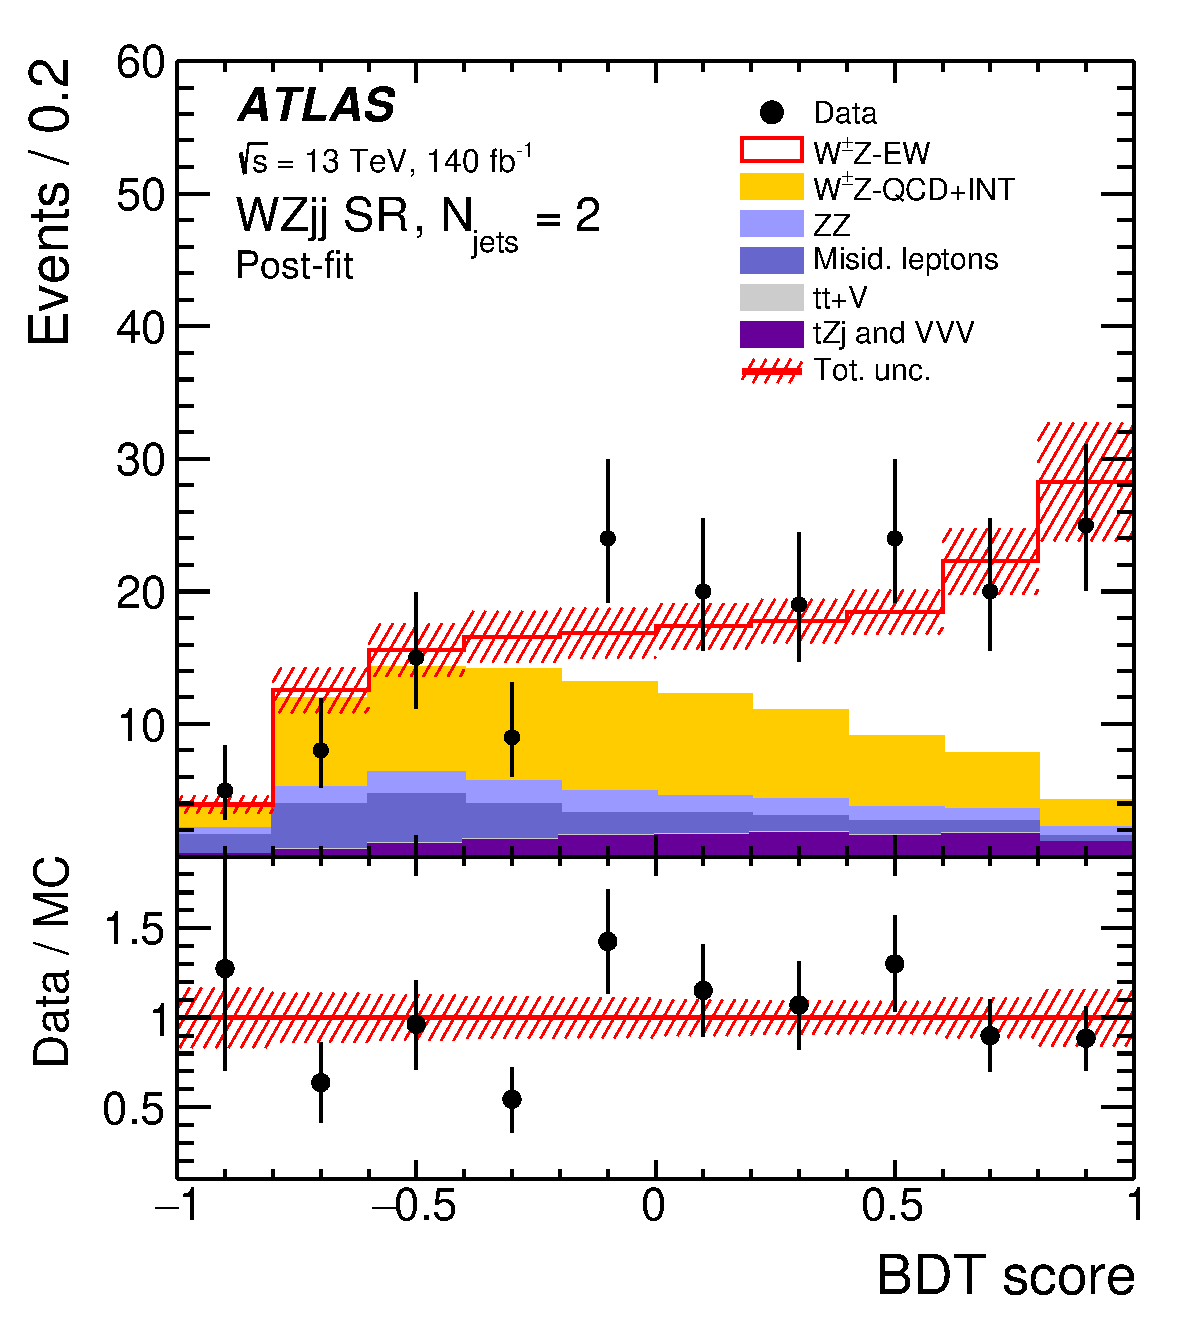
\includegraphics[width=0.4\textwidth]{Immagini/fig_03a.pdf}
}
\subfloat[]{
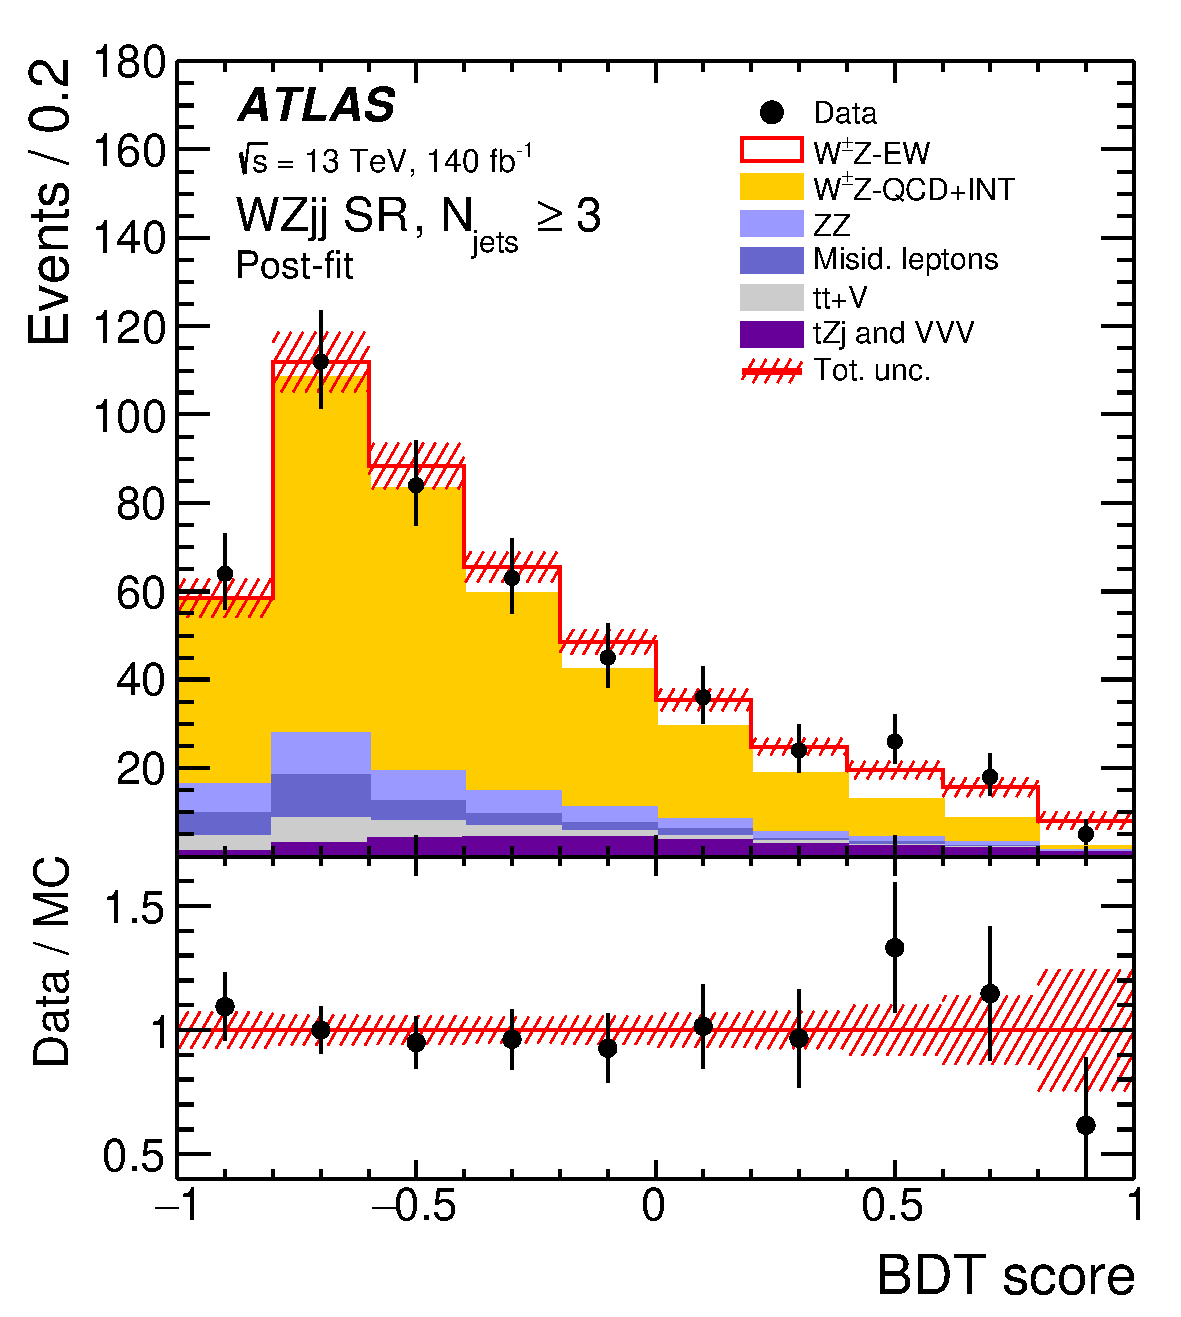
\includegraphics[width=0.4\textwidth]{Immagini/fig_03b.pdf}
}\\
\subfloat[]{
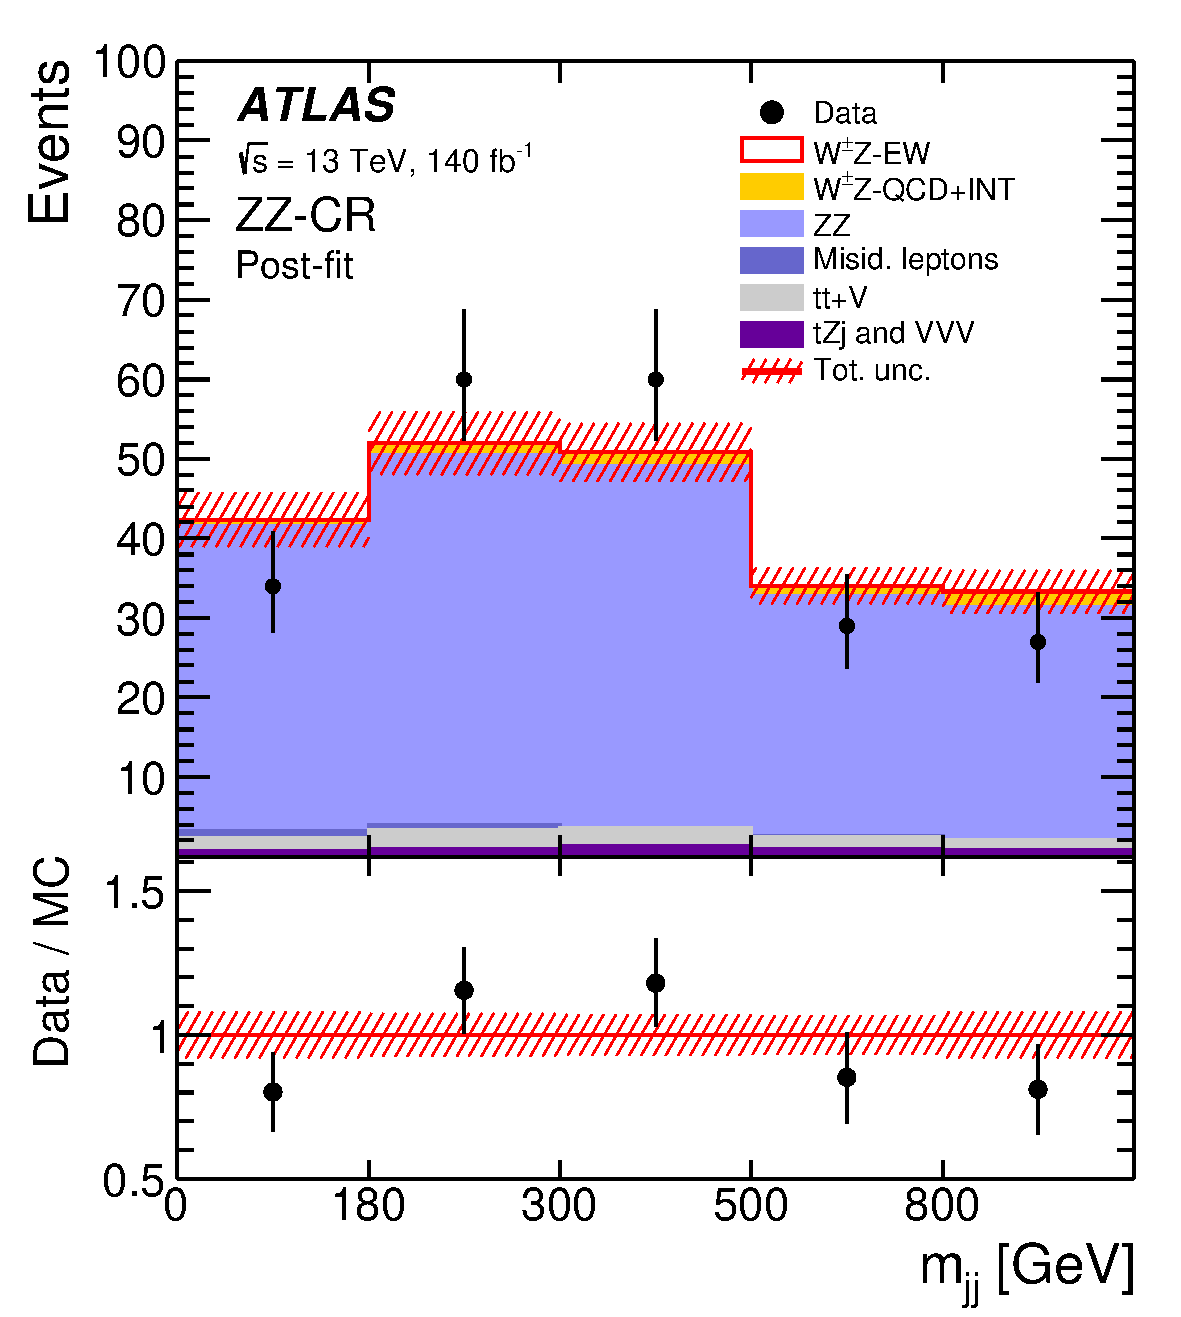
\includegraphics[width=0.4\textwidth]{Immagini/fig_03c.pdf}
}
\subfloat[]{
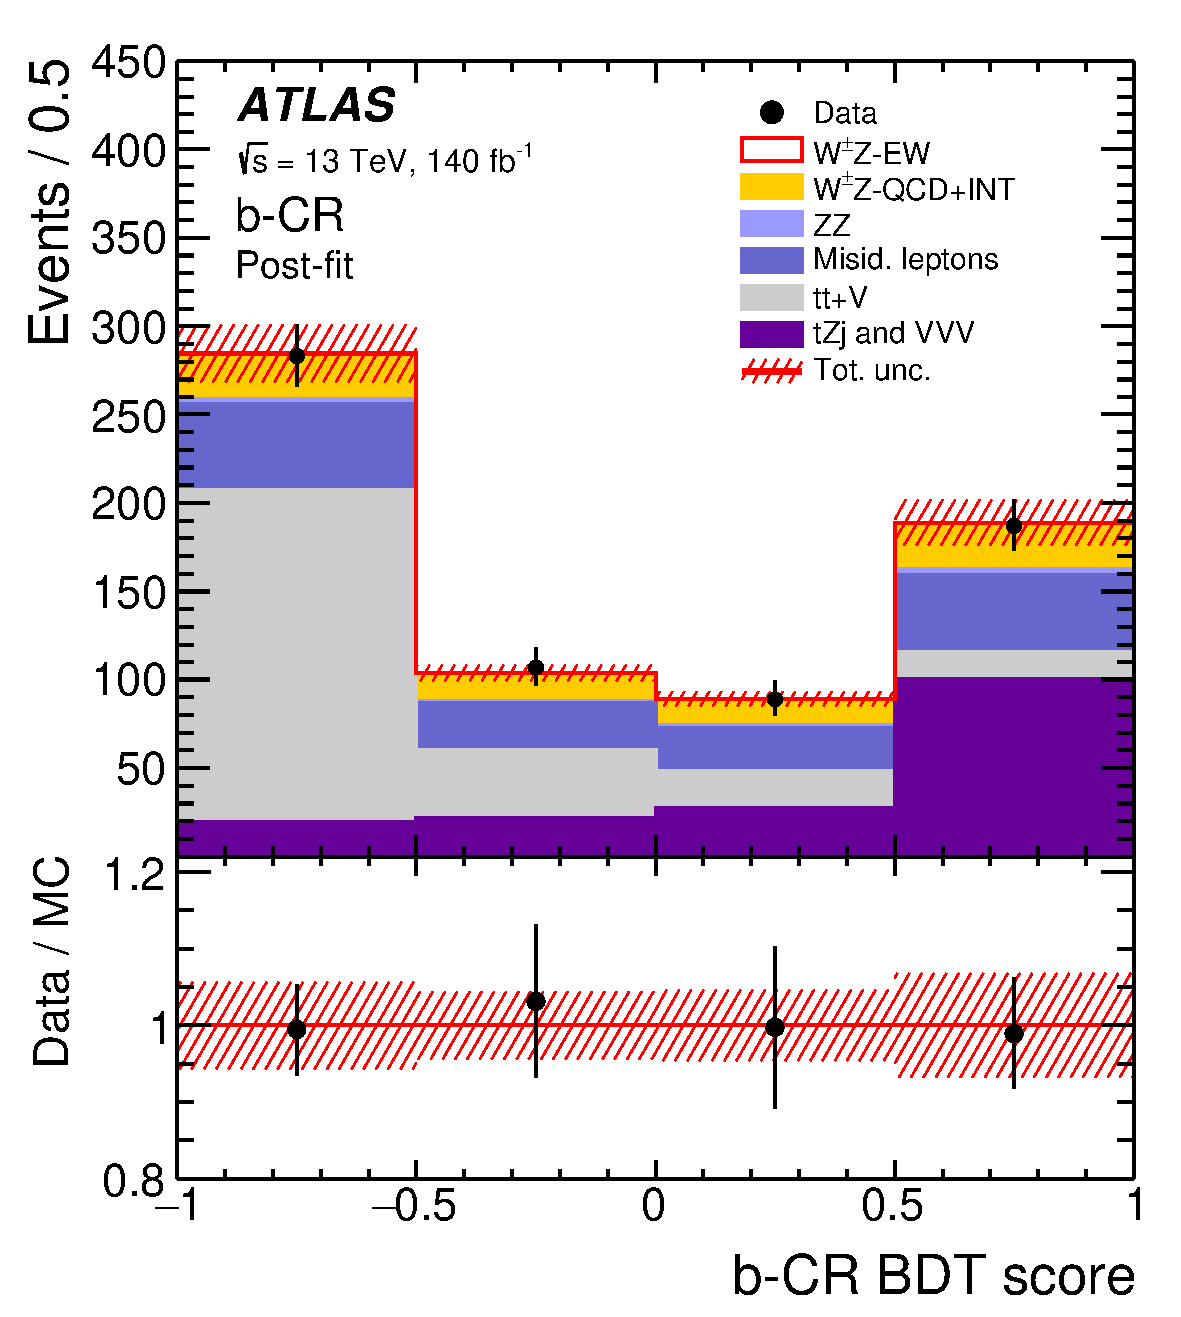
\includegraphics[width=0.4\textwidth]{Immagini/fig_03d.pdf}
}
\caption{Distribuzioni post-fit: (a) \textit{score} del BDT nella regione di segnale per la categoria $N_{\text{jet}} = 2$, (b) \textit{score} del BDT per la categoria $N_{\text{jet}} \ge 3$, (c) \mjj\ nella regione di controllo $ZZ$-CR, e (d) \textit{score} del BDT della $b$-CR nella regione di controllo $b$-CR. Il segnale e i fondi sono normalizzati al numero di eventi attesi dopo il fit. La banda di incertezza attorno all'aspettazione del MC include tutte le incertezze sistematiche ottenute dal fit.}
\label{fig:BDTScore}
\end{figure}

\begin{table}[htbp] 
\centering
\renewcommand{\arraystretch}{1.4}
\begin{tabular}{l c c c c}
\hline
\textbf{Processo} & \textbf{SR ($N_{\text{jet}} = 2$)} & \textbf{SR ($N_{\text{jet}} \ge 3$)} & \textbf{$b$-CR} & \textbf{$ZZ$-CR} \\
\hline
\hline
\textbf{Dati osservati} & 169 & 477 & 666 & 210 \\
\textbf{Totale atteso} & 170 $\pm$ 13 & 476 $\pm$ 22 & 667 $\pm$ 26 & 212 $\pm$ 14 \\
\hline
\wzjjew & 68 $\pm$ 14 & 55 $\pm$ 18 & 4.84 $\pm$ 0.27 & 0.724 $\pm$ 0.014 \\
\wzjjqcd & 58 $\pm$ 16 & 307 $\pm$ 27 & 77 $\pm$ 18 & 6.3 $\pm$ 0.7 \\
\wzjj-INT & 0.9 $\pm$ 0.4 & 4.4 $\pm$ 2.3 & 0.57 $\pm$ 0.29 & 0.22 $\pm$ 0.11 \\
$t\bar{t}+V$ & 0.59 $\pm$ 0.10 & 18.3 $\pm$ 2.4 & 262 $\pm$ 34 & 9.0 $\pm$ 1.3 \\
$tZj$ & 11.0 $\pm$ 1.9 & 25 $\pm$ 5 & 169 $\pm$ 30 & 0.54 $\pm$ 0.09 \\
$ZZ$-QCD & 10.3 $\pm$ 1.0 & 34.6 $\pm$ 3.2 & 10.1 $\pm$ 0.5 & 171 $\pm$ 15 \\
$ZZ$-EW & 1.9 $\pm$ 0.4 & 3.7 $\pm$ 0.9 & 0.21 $\pm$ 0.05 & 19 $\pm$ 5 \\
$VVV$ & 0.41 $\pm$ 0.10 & 2.0 $\pm$ 0.5 & 0.39 $\pm$ 0.10 & 4.2 $\pm$ 1.0 \\
Leptoni \textit{fake} & 18 $\pm$ 4 & 27 $\pm$ 6 & 143 $\pm$ 35 & 1.7 $\pm$ 0.5 \\
\hline
\end{tabular}
\caption{Numero di eventi osservati e attesi nella regione di segnale (SR) per la produzione di $W^\pm Zjj$ e nelle due regioni di controllo, dopo l'esecuzione del fit. Vengono mostrati i conteggi post-fit per i segnali e per i processi di fondo. La categoria ``Leptoni \textit{fake}'' raggruppa i fondi con leptoni misidentificati. Vengono riportate le incertezze sistematiche totali post-fit correlate.}
\label{tab:VBSyield_postfit}
\end{table}

Le distribuzioni post-fit dello \textit{score} del BDT nella regione di segnale per gli eventi con $N_{\text{jet}} = 2$ e $N_{\text{jet}} \ge 3$ sono presentate rispettivamente nelle Figure \ref{fig:BDTScore}(a) e (b). Le normalizzazioni dei fondi, del segnale e i parametri di disturbo (\textit{nuisance parameters}) sono regolati tramite il fit di verosimiglianza profilata (\textit{profile-likelihood fit}). Le distribuzioni post-fit di \mjj\ nella $ZZ$-CR e dello \textit{score} del BDT della $b$-CR nella $b$-CR sono presentate nelle Figure \ref{fig:BDTScore}(c) e (d). Le corrispondenti rese degli eventi post-fit sono dettagliate nella Tabella \ref{tab:VBSyield_postfit}. 

I parametri di normalizzazione dei fondi $t\bar{t}V$ e $ZZ$, vincolati dai dati nelle regioni di controllo e di segnale, sono misurati essere $\mu_{t\bar{t}V} = 0.91 \pm 0.13$, $\mu_{tZj} = 1.26 \pm 0.22$ e $\mu_{ZZ} = 1.07 \pm 0.11$. Non si osserva alcuno spostamento (\textit{pull}) dei parametri di disturbo superiore a $0.5\sigma$.

Le sezioni d'urto fiduciali integrate $\sigma_{\text{EW}}$ e $\sigma_{\text{strong}}$, per un dato canale di decadimento $W^\pm Z \rightarrow \ell'^{\pm}\nu\ell^+\ell^-$, dove $\ell$ e $\ell'$ rappresentano un elettrone o un muone, sono misurate essere:
\begin{align*}
\sigma_{\text{EW}} &= 0.368 \pm 0.037\,\text{(stat.)} \pm 0.059\,\text{(syst.)} \pm 0.003\,\text{(lumi.)} \unit{fb} = 0.37 \pm 0.07\,\unit{fb} \\
\sigma_{\text{strong}} &= 1.093 \pm 0.066\,\text{(stat.)} \pm 0.131\,\text{(syst.)} \pm 0.009\,\text{(lumi.)} \unit{fb} = 1.09 \pm 0.14\,\unit{fb}
\end{align*}
dove le incertezze corrispondono, nell'ordine, all'errore statistico, sistematico e della luminosità. 

La Tabella \ref{table:sysOnMu_summary} mostra le principali sorgenti di incertezza sulle sezioni d'urto misurate. La precisione delle misure è limitata dalle incertezze sistematiche, e in particolare dalle incertezze di modellizzazione dei generatori di eventi MC. Le incertezze sistematiche totali risentono inoltre delle correlazioni esistenti tra le sezioni d'urto misurate $\sigma_{\text{EW}}$ e $\sigma_{\text{strong}}$, che sono dell'ordine del $36\%$.

Le corrispondenti previsioni teoriche calcolate da \textsc{MadGraph5\_aMC@NLO}+\textsc{Pythia8} (\textsc{MGPy8}) sono:
\begin{align*}
\sigma_{\text{EW}}^{\textsc{MGPy8}} &= 0.370 \pm 0.001\,\text{(stat.)} \pm 0.006\,\text{(PDF)} \; ^{+0.030}_{-0.026}\,\text{(scala)} \unit{fb} \\
\sigma_{\text{strong}}^{\textsc{MGPy8}} &= 1.537 \pm 0.009\,\text{(stat.)} \pm 0.016\,\text{(PDF)} \; ^{+0.087}_{-0.149}\,\text{(scala)} \unit{fb}
\end{align*}
dove le incertezze corrispondono rispettivamente all'errore statistico, alle PDF e alle scale di QCD.

\begin{figure}[htbp]
\centering
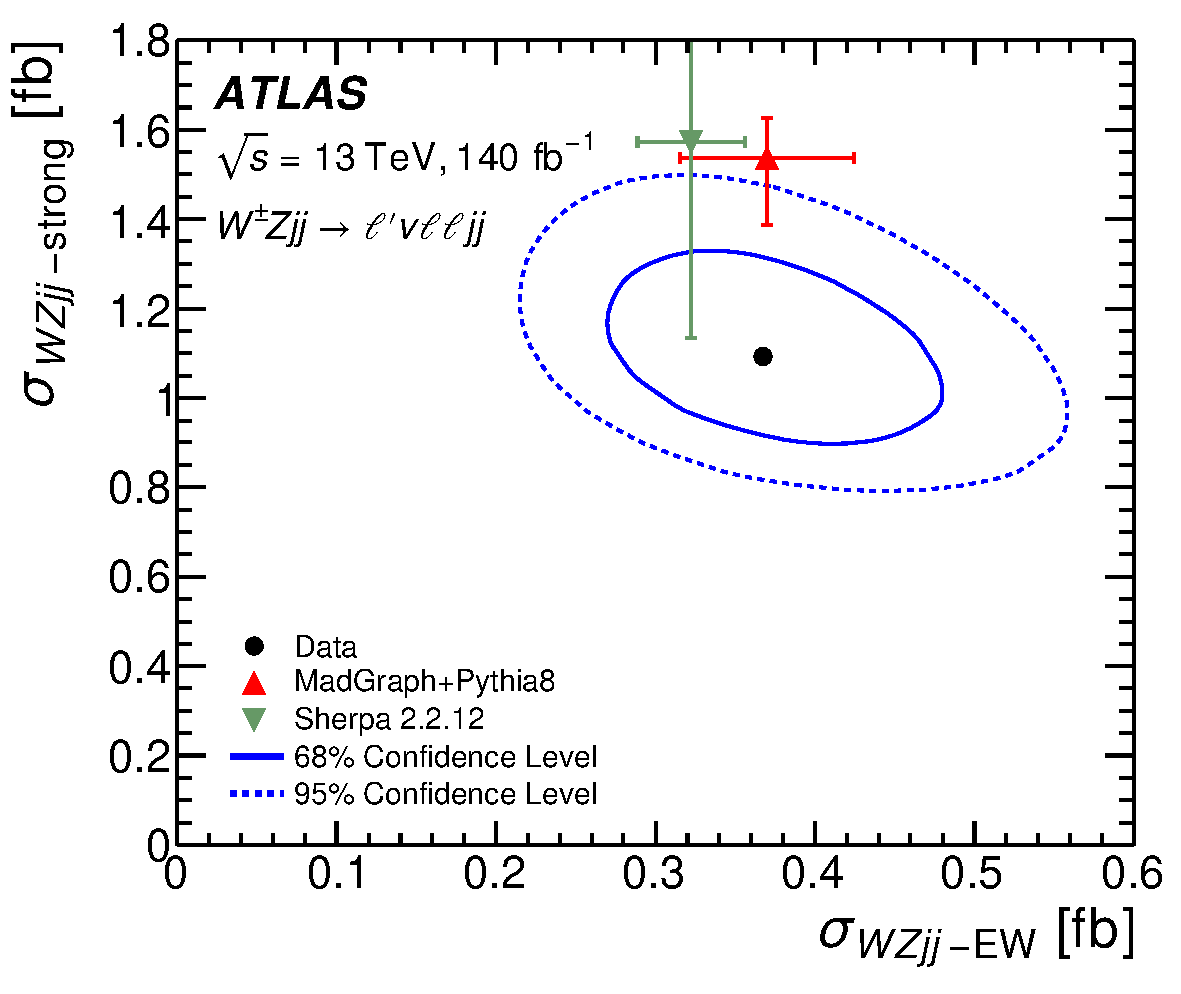
\includegraphics[width=0.49\textwidth]{Immagini/fig_04.pdf}
\caption{Misure delle sezioni d'urto integrate $\sigma_{\text{EW}}$ e $\sigma_{\text{strong}}$ confrontate con le previsioni di \textsc{MGPy8} (triangolo rivolto verso l'alto) e \textsc{Sherpa} 2.2.12 (triangolo rivolto verso il basso). I contorni continui e tratteggiati attorno ai punti sperimentali corrispondono rispettivamente al $68\%$ e al $95\%$ CL.}
\label{fig:2DContour_sigew_sigqcd_All_data}
\end{figure}

I valori misurati di $\sigma_{\text{EW}}$ e $\sigma_{\text{strong}}$ sono confrontati con le previsioni di \textsc{MGPy8} e \textsc{Sherpa}~2.2.12 nella Figura \ref{fig:2DContour_sigew_sigqcd_All_data}. Si osserva un ottimo accordo tra le predizioni MC e la sezione d'urto integrata di \wzjjew, mentre la sezione d'urto integrata di \wzjj-strong misurata risulta inferiore rispetto alle predizioni di entrambi i generatori MC di un fattore pari a $0.7$. Considerando l'incertezza teorica nella predizione di \textsc{MGPy8}, la misura attuale e la stima teorica concordano entro $1.8\sigma$. Un'osservazione simile riguardo alla sovrastima della modellizzazione della produzione forte di $WZjj$ è stata riscontrata dalla collaborazione ATLAS anche in uno spazio delle fasi differente, ed è coerente con le misure effettuate nelle precedenti pubblicazioni di ATLAS dedicate agli stati finali $WZjj$ e $WZ$.

La sezione d'urto integrata totale di \wzjj\ nello spazio delle fasi fiduciale viene estratta dal fit ed è pari a $\sigma_{\text{tot}} = 1.462 \pm 0.133\,\unit{fb} = 1.462 \pm 0.063\,\text{(stat.)} \pm 0.118\,\text{(sys.)} \pm 0.012\,\text{(lumi.)} \unit{fb}$. La corrispondente predizione di \textsc{MGPy8} per la somma delle componenti forte ed elettrodebole (inclusi gli effetti di interferenza) è di $1.907 \pm 0.009\,\text{(stat.)} \pm 0.022\,\text{(PDF)} \; ^{+0.117}_{-0.175}\,\text{(scala)} \unit{fb}$.


\subsection{Misure differenziali di WZjj-EW\ e WZjj-strong}
\label{sec:results_ew_diff}

Dividendo la regione di segnale in eventi con $N_{\text{jet}} = 2$ e $N_{\text{jet}} \ge 3$, vengono misurate le sezioni d'urto di produzione $\sigma_{\text{EW}}$ e $\sigma_{\text{strong}}$ per queste due categorie. Le misure sono confrontate nella Figura \ref{fig:2DContour_sigew_sigqcd_Nj_data} con le predizioni di \textsc{MGPy8} e \textsc{Sherpa}~2.2.12. 

Per la categoria $N_{\text{jet}} \ge 3$, le sezioni d'urto elettrodeboli predette sono in buon accordo con il valore misurato, mentre la sezione d'urto forte predetta si trova entro circa $2\sigma$ dalla misura. Tuttavia, per la categoria $N_{\text{jet}} = 2$, la sezione d'urto forte misurata è inferiore di un fattore due rispetto al valore previsto sia da \textsc{MGPy8} che da \textsc{Sherpa}. I valori predetti di $\sigma_{\text{EW}}$ risultano in accordo entro $1\sigma$ con il valore misurato.

\begin{figure}[htbp]
\centering
\subfloat[]{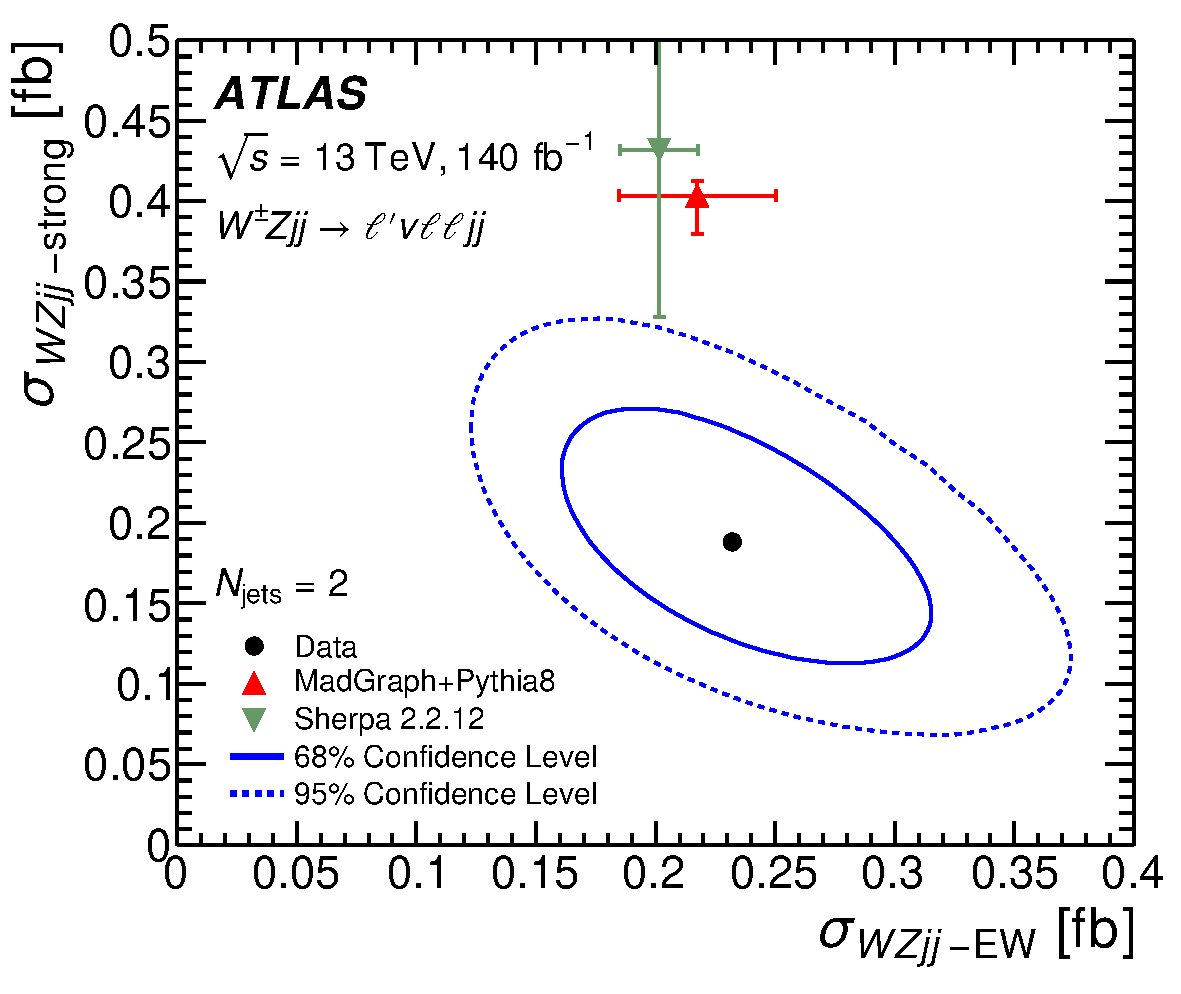
\includegraphics[width=0.49\textwidth]{Immagini/fig_05a.pdf}}
\subfloat[]{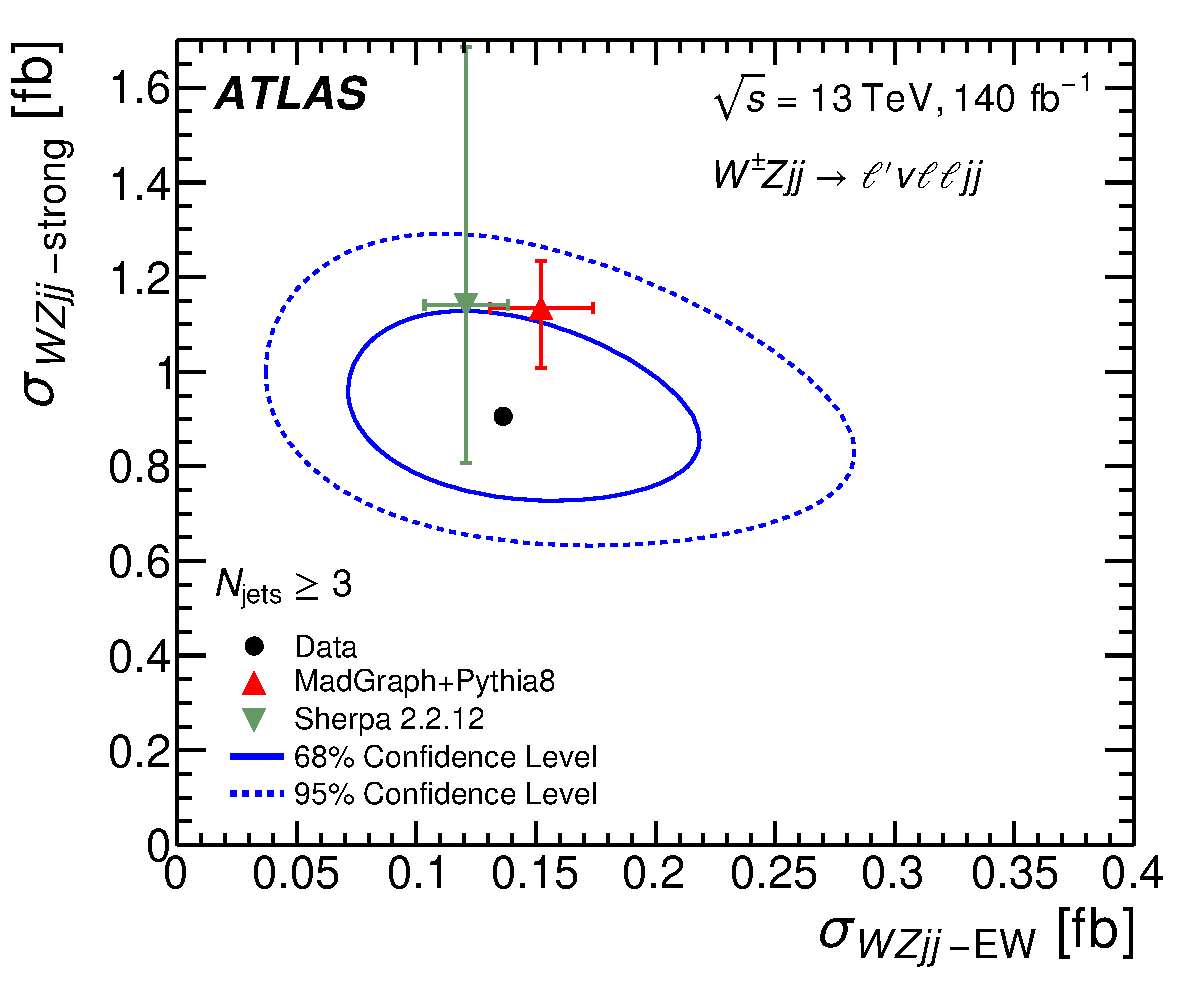
\includegraphics[width=0.49\textwidth]{Immagini/fig_05b.pdf}}
\caption{Sezioni d'urto misurate $\sigma_{\text{EW}}$ e $\sigma_{\text{strong}}$ per le categorie (a) $N_{\text{jet}} = 2$ e (b) $N_{\text{jet}} \ge 3$, confrontate con le previsioni di \textsc{MGPy8} e \textsc{Sherpa}~2.2.12. I contorni continui e tratteggiati corrispondono al $68\%$ e $95\%$ CL.}
\label{fig:2DContour_sigew_sigqcd_Nj_data}
\end{figure}

Il rapporto $R_{2/3}$ tra il numero di eventi con $N_{\text{jet}} = 2$ e il numero di eventi con $N_{\text{jet}} \ge 3$ viene estratto dai dati tramite il fit simultaneo delle due categorie, ottenendo $R_{\text{EW}} = 1.70 \pm 0.71$ e $R_{\text{strong}} = 0.21 \pm 0.06$, rispettivamente per i processi elettrodeboli e forti. In confronto, i valori predetti da \textsc{MGPy8} (\textsc{Sherpa}) sono $R_{\text{EW}} = 1.43^{+0.06}_{-0.02}\;(1.67 \pm 0.13)$ e $R_{\text{strong}} = 0.36^{+0.02}_{-0.04}\;(0.38 \pm 0.03)$.

Le sezioni d'urto di produzione $\sigma_{\text{EW}}$ e $\sigma_{\text{strong}}$ sono misurate in modo differenziale anche in tre \textit{bin} della variabile \mjj. Le misure sono confrontate nella Figura \ref{fig:2DContour_sigew_sigqcd_mjj_data} con le predizioni di \textsc{MGPy8} e \textsc{Sherpa}~2.2.12. Per l'intervallo $500 < \mjj < 1300\,\unit{GeV}$, le predizioni dei MC sovrastimano il valore di $\sigma_{\text{strong}}$ misurato di un fattore $1.4$. Per valori di \mjj\ superiori a $1300\,\unit{GeV}$, le predizioni dei MC concordano entro circa $2\sigma$ con le misure per entrambe le componenti.

\begin{figure}[htbp]
\centering
\subfloat[]{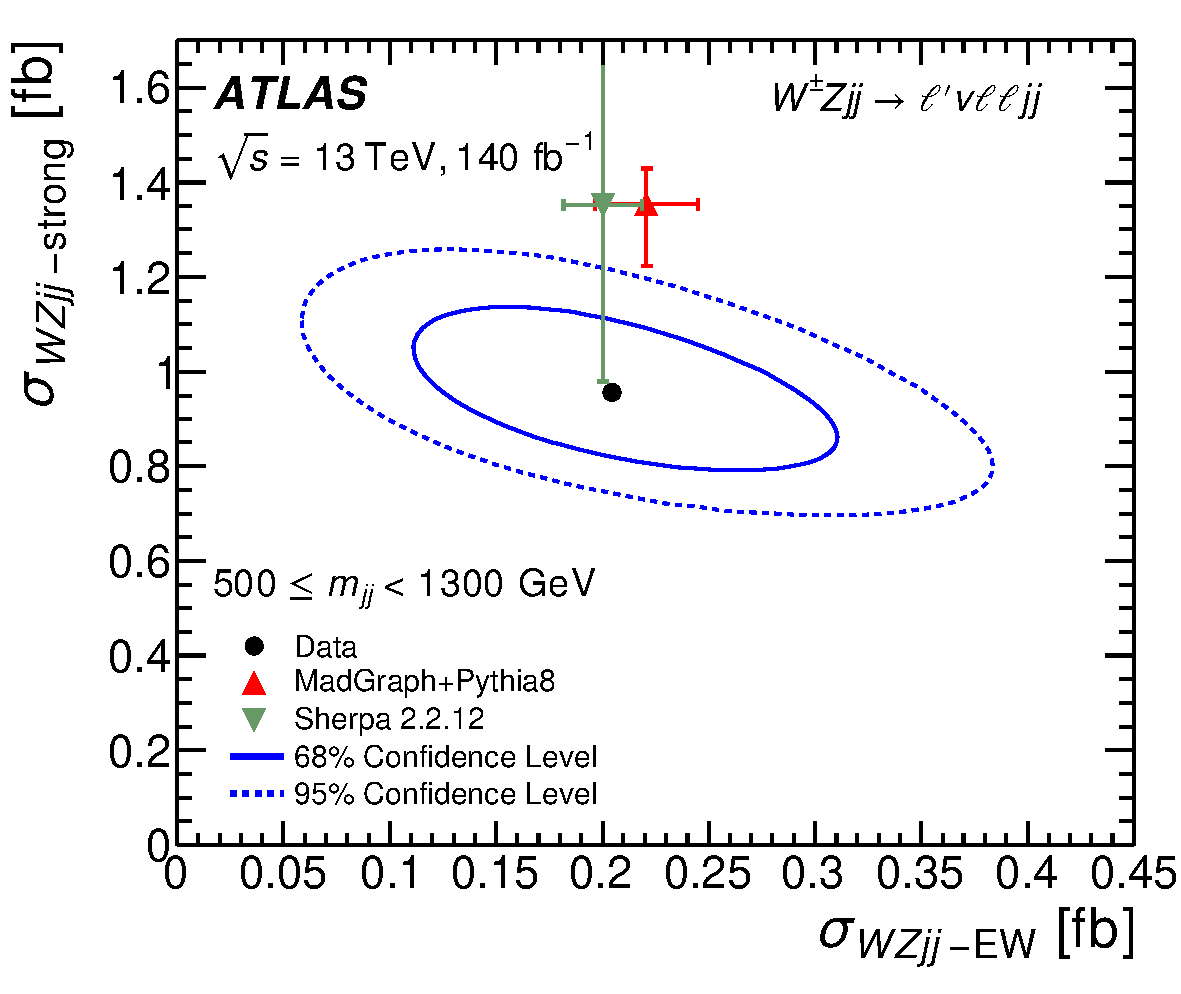
\includegraphics[width=0.45\textwidth]{Immagini/fig_06a.pdf}}
\subfloat[]{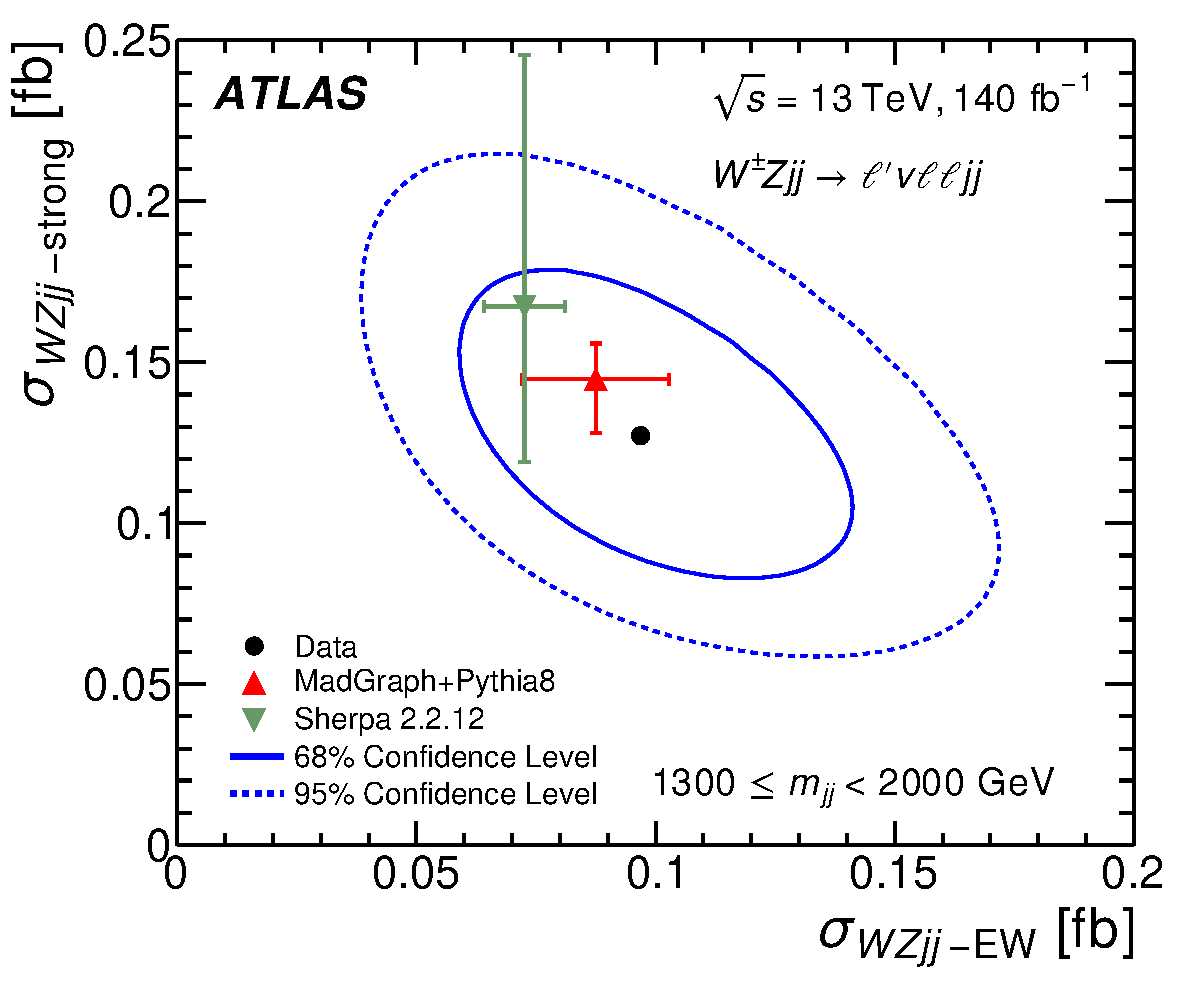
\includegraphics[width=0.45\textwidth]{Immagini/fig_06b.pdf}}\\
\subfloat[]{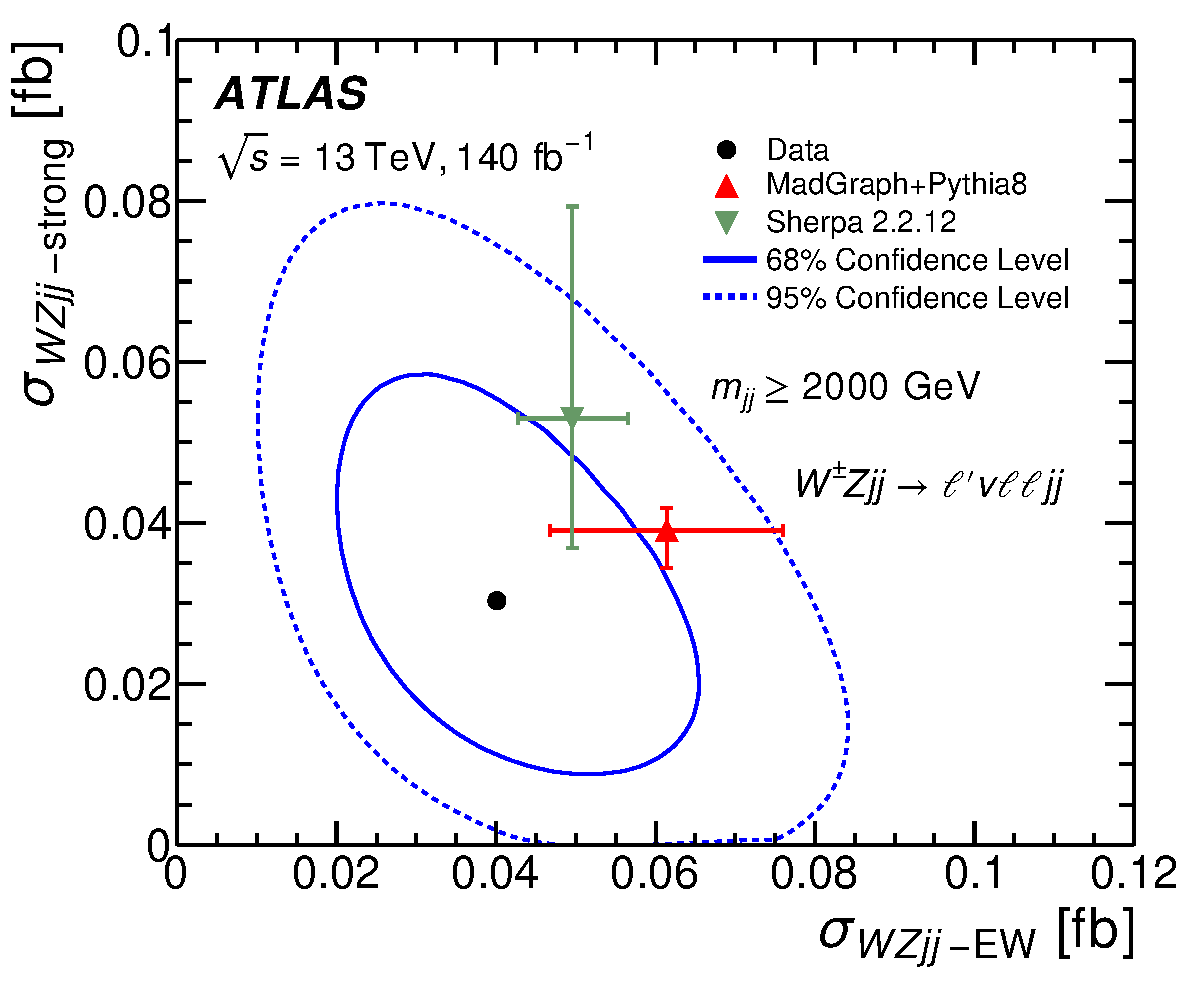
\includegraphics[width=0.45\textwidth]{Immagini/fig_06c.pdf}}
\caption{Sezioni d'urto misurate $\sigma_{\text{EW}}$ e $\sigma_{\text{strong}}$ per ciascun bin di \mjj: (a) $500 \le \mjj < 1300\,\unit{GeV}$, (b) $1300 \le \mjj < 2000\,\unit{GeV}$, e (c) $\mjj \ge 2000\,\unit{GeV}$, confrontate con le predizioni teoriche. I contorni indicano il $68\%$ e il $95\%$ CL.}
\label{fig:2DContour_sigew_sigqcd_mjj_data}
\end{figure}


\subsection{Misure differenziali inclusive di WZjj}
\label{sec:wzjj_diff_results}

\begin{figure}[htbp]
\centering
\subfloat[]{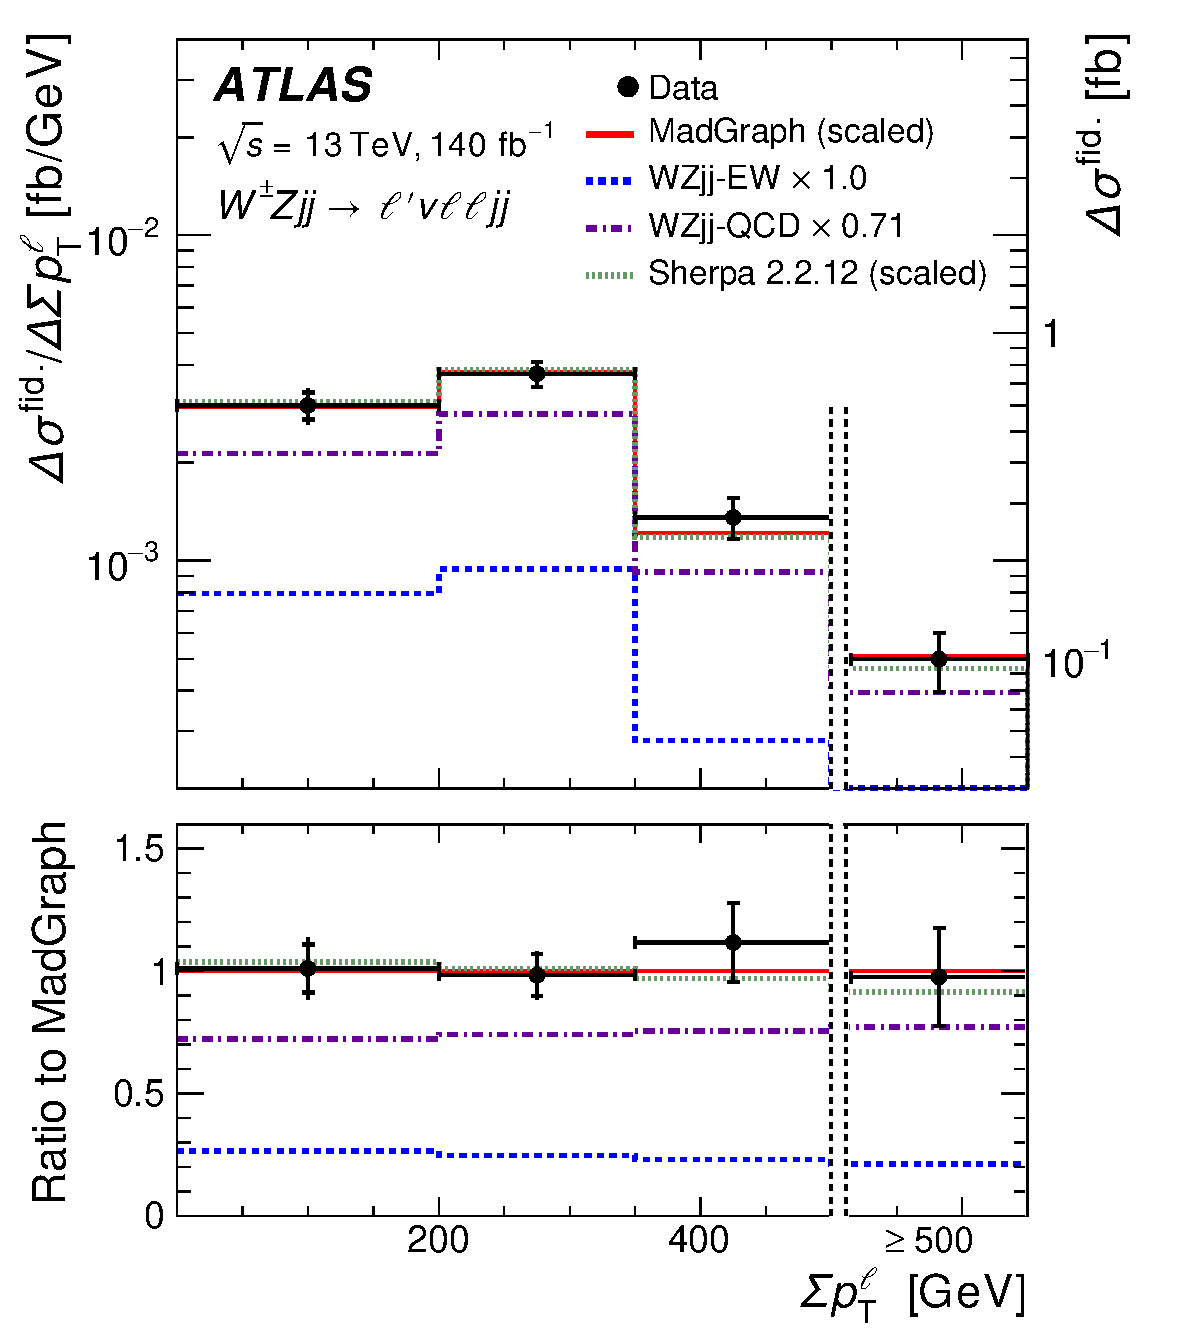
\includegraphics[width=0.45\textwidth]{Immagini/fig_07a.pdf}}
\subfloat[]{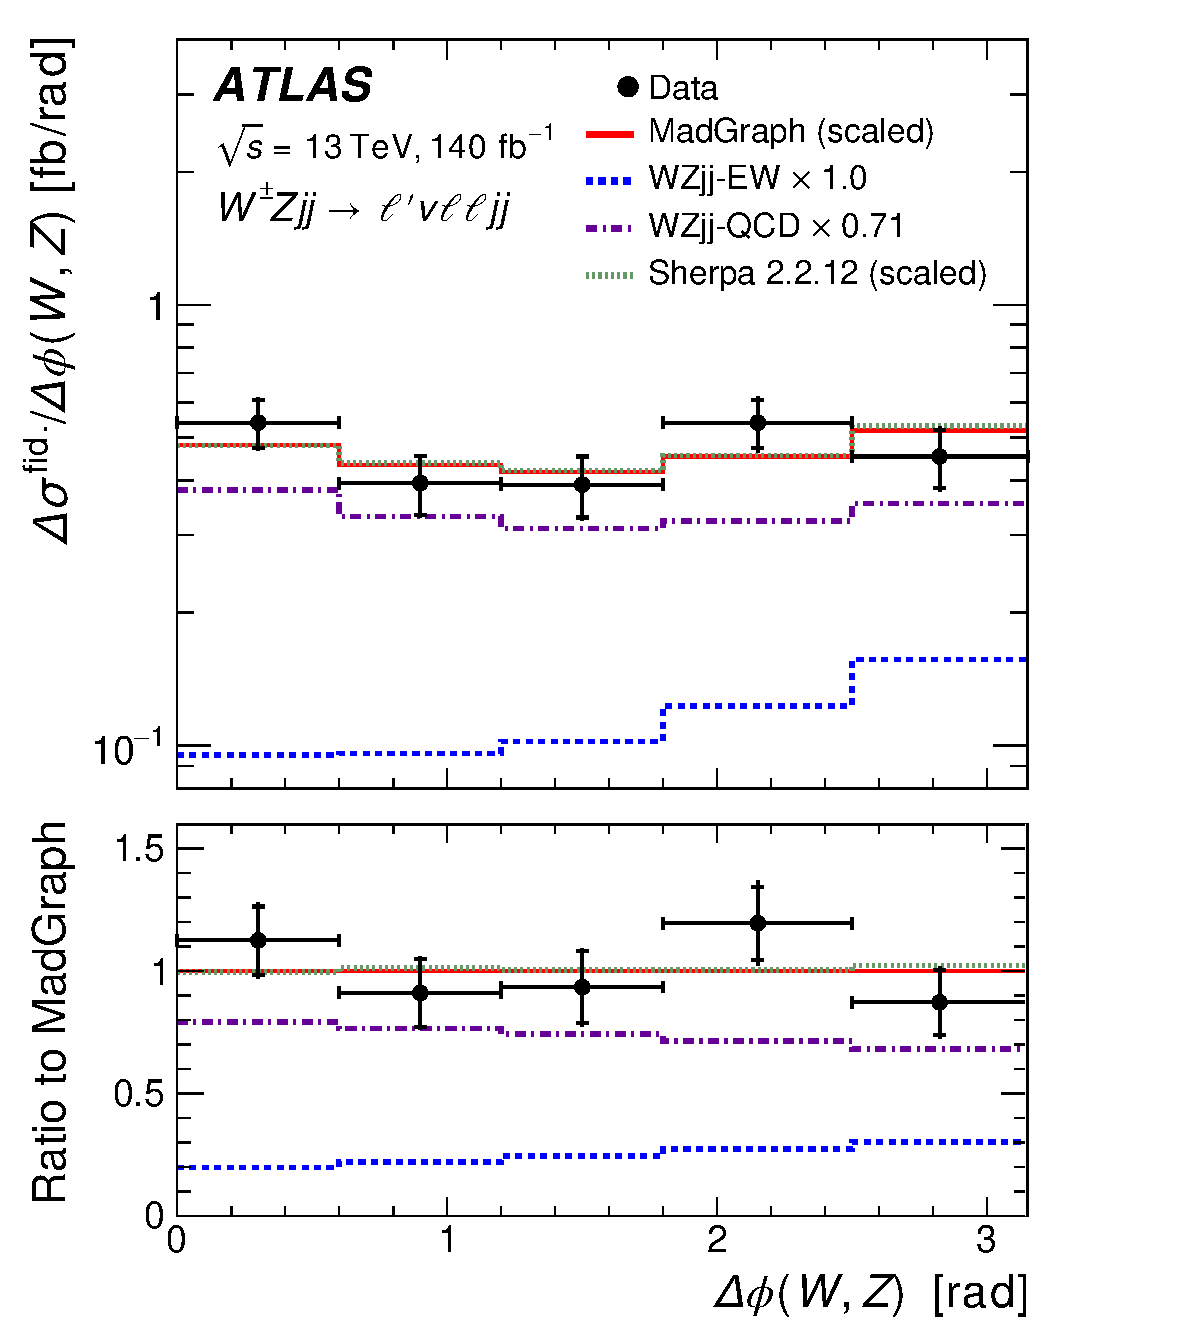
\includegraphics[width=0.45\textwidth]{Immagini/fig_07b.pdf}}\\
\subfloat[]{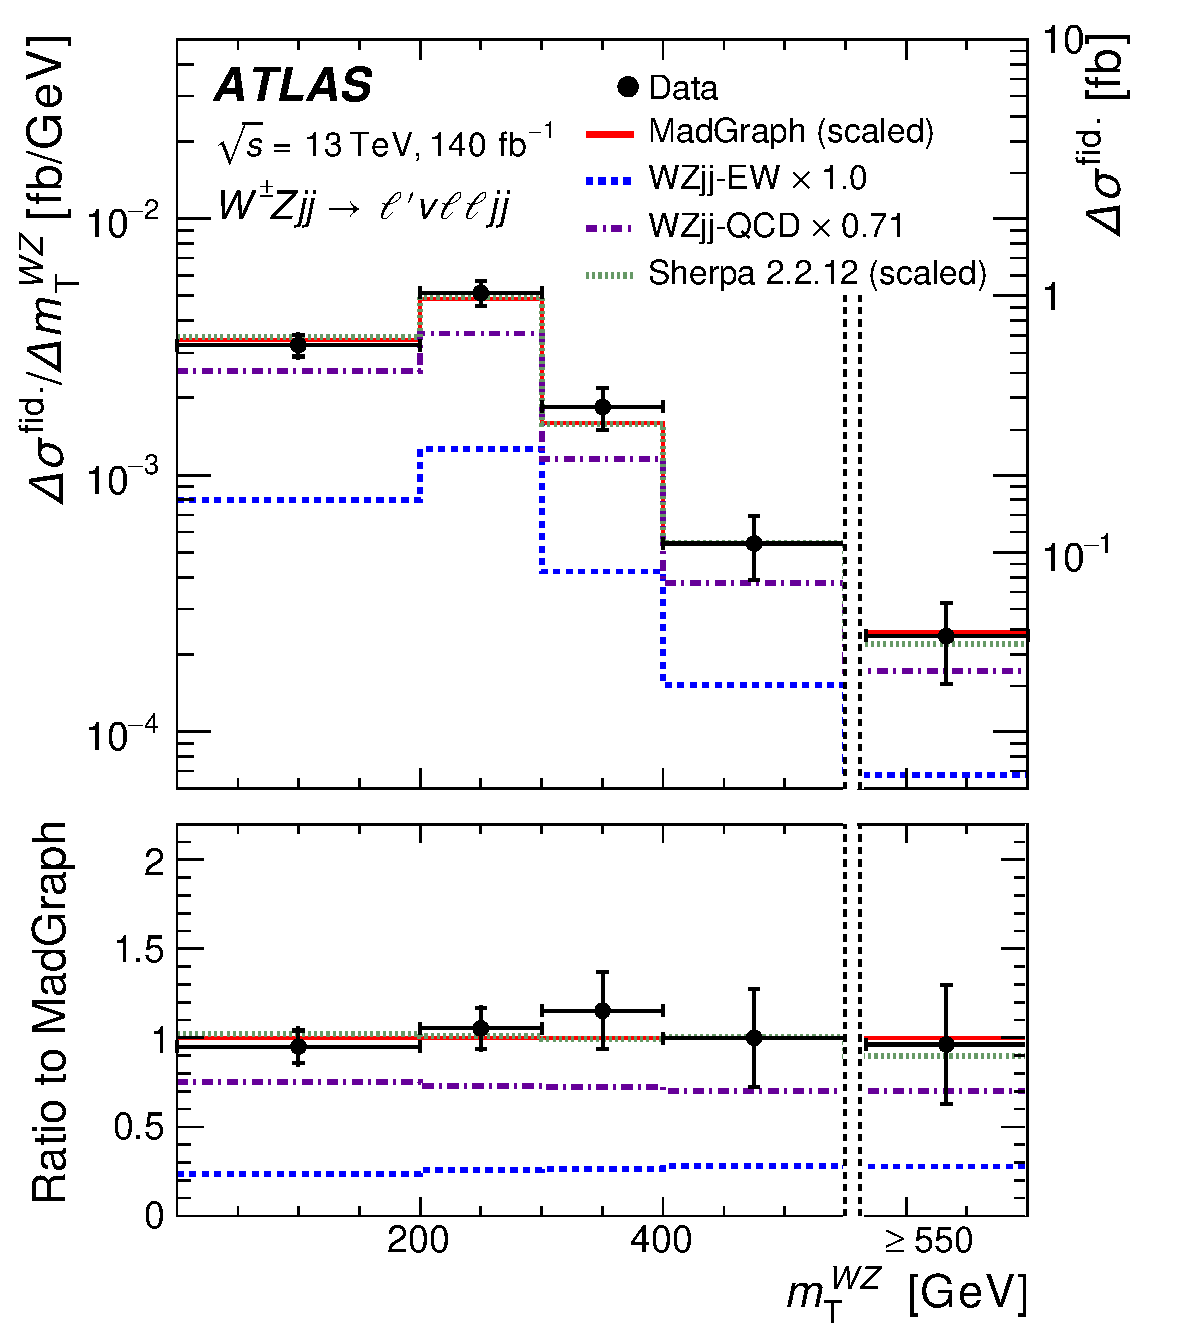
\includegraphics[width=0.45\textwidth]{Immagini/fig_07c.pdf}}
\caption{Sezione d'urto differenziale inclusiva di \wzjj\ misurata nello spazio delle fasi fiduciale del VBS in funzione di: (a) $\sum p_T^\ell$ (somma scalare dei $p_T$ dei tre leptoni), (b) $\Delta\phi(W,Z)$ e (c) \mtwz\ (massa trasversa del sistema $WZ$). Le barre di errore interne ed esterne sui punti dati rappresentano rispettivamente le incertezze statistiche e totali. Le misure sono confrontate con la somma delle predizioni riscalate di \textsc{MGPy8} (linea continua) e \textsc{Sherpa}~2.2.12 (linea punteggiata). I contributi separati di \wzjjew\ e \wzjjqcd\ sono rappresentati rispettivamente dalle linee tratteggiate e tratto-punto. In (a) e (c), l'asse $y$ destro si riferisce all'ultimo bin (separato da una linea verticale tratteggiata), che è integrato fino al valore massimo raggiunto nello spazio delle fasi. I pannelli inferiori mostrano i rapporti tra i dati e le predizioni di \textsc{MGPy8}.}
\label{fig:diffXSection:SptL_dPhiWZ}
\end{figure}


\begin{figure}[htbp]
\centering
\subfloat[]{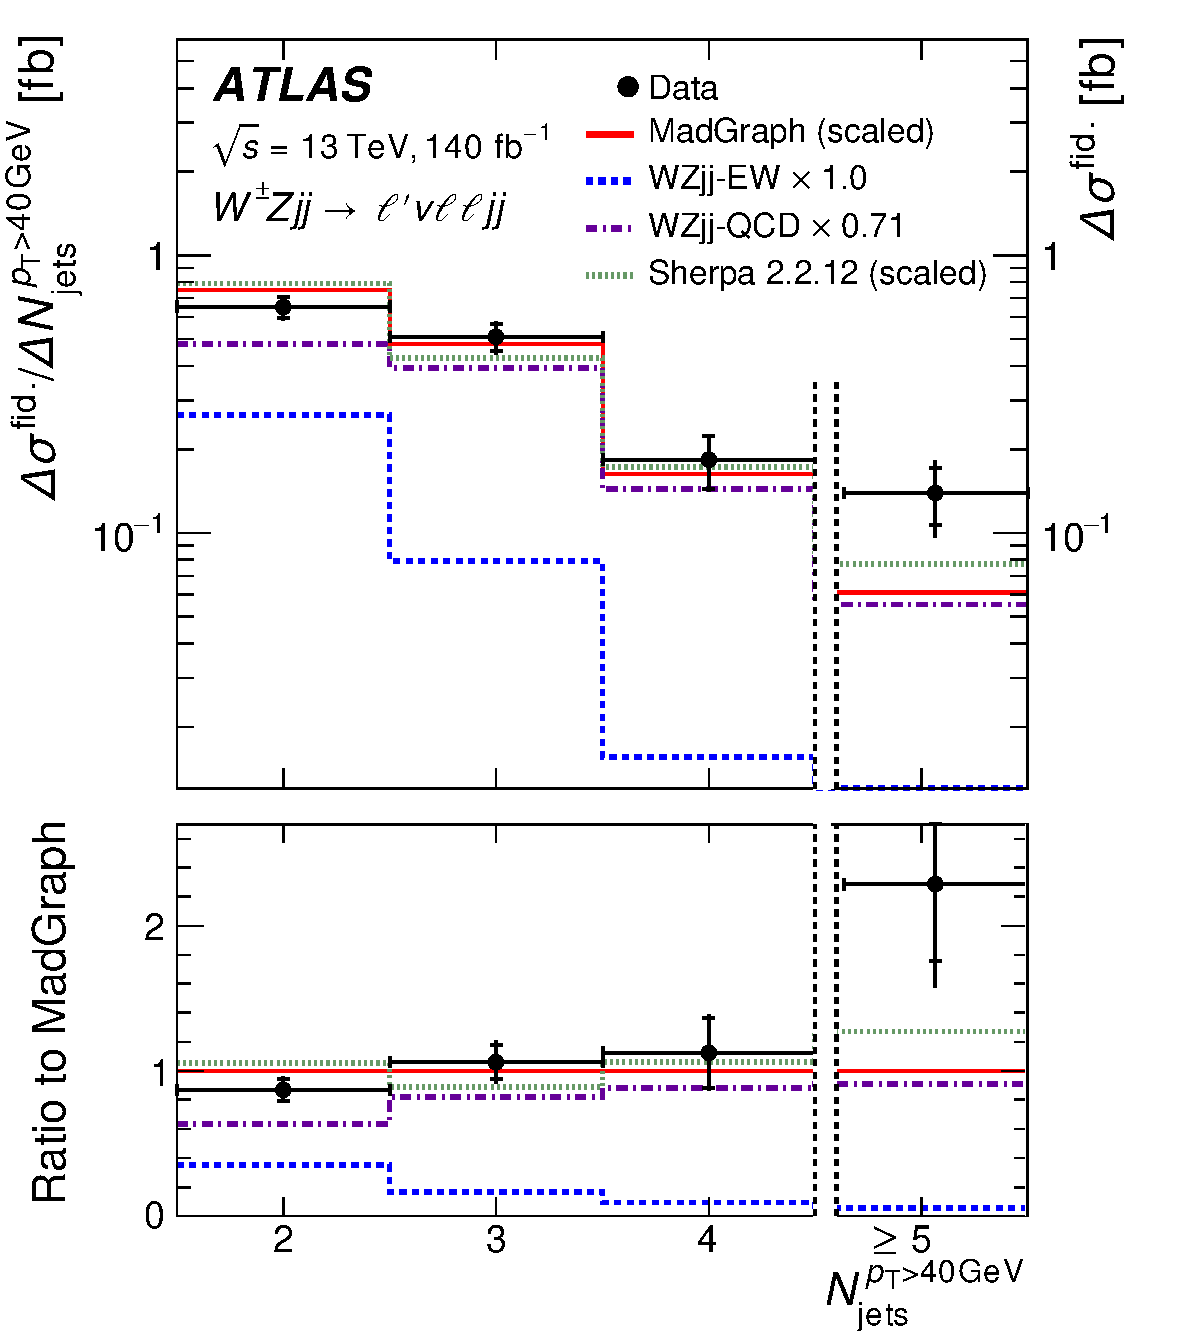
\includegraphics[width=0.45\textwidth]{Immagini/fig_08a.pdf}}
\subfloat[]{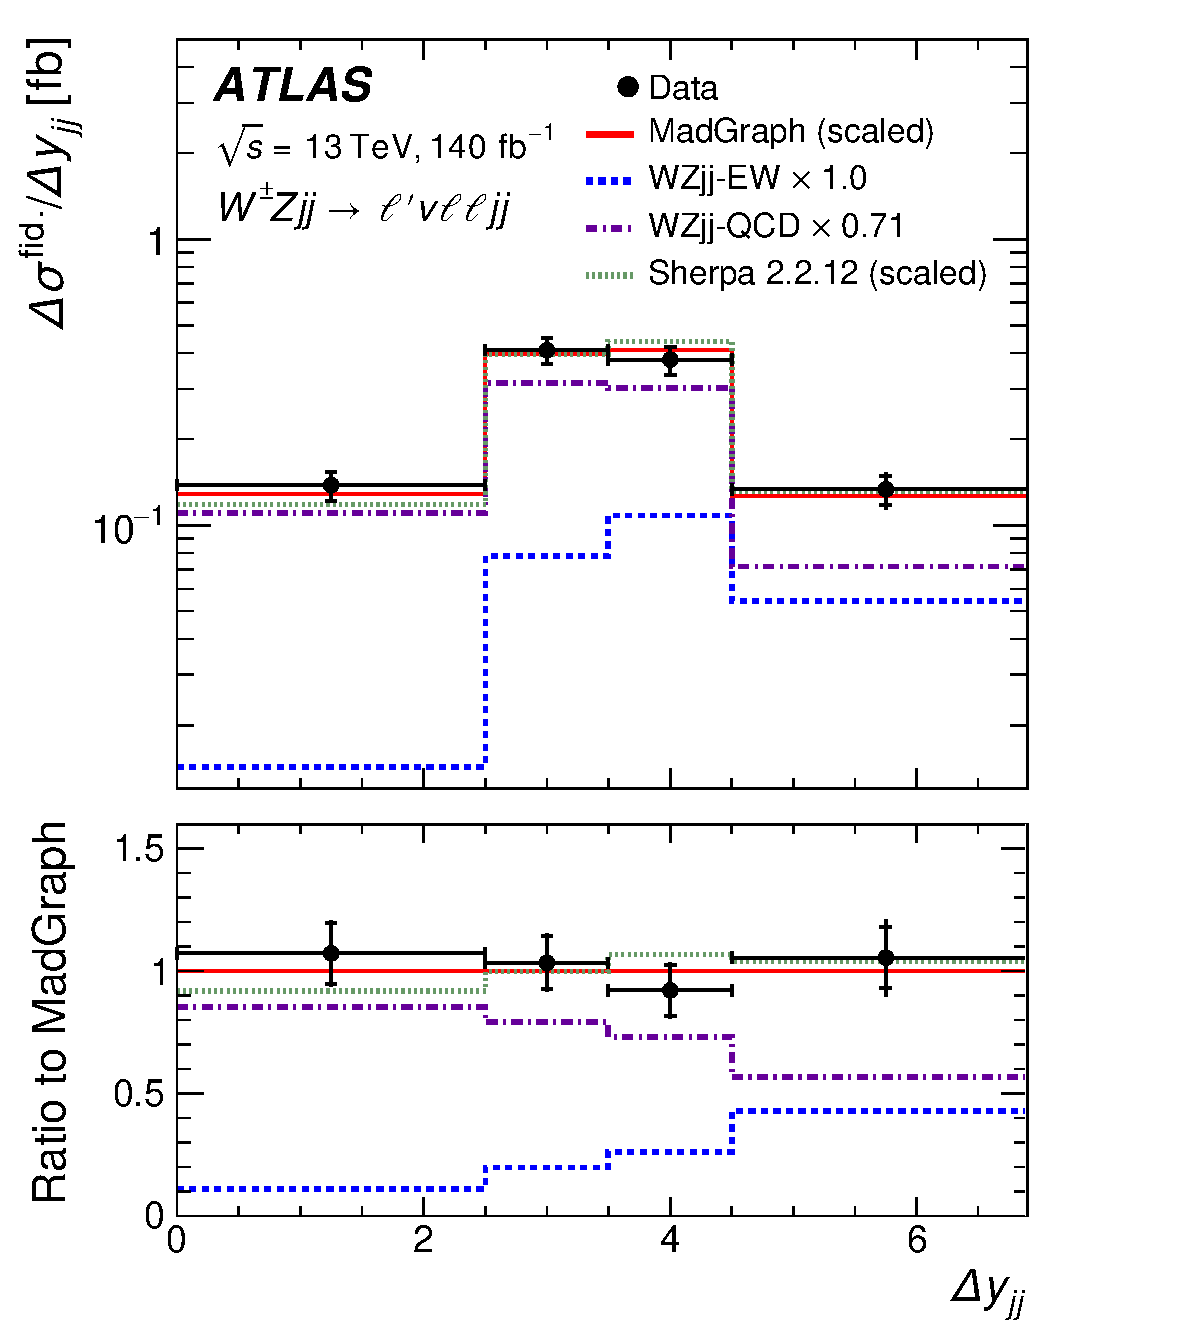
\includegraphics[width=0.45\textwidth]{Immagini/fig_08b.pdf}}\\
\subfloat[]{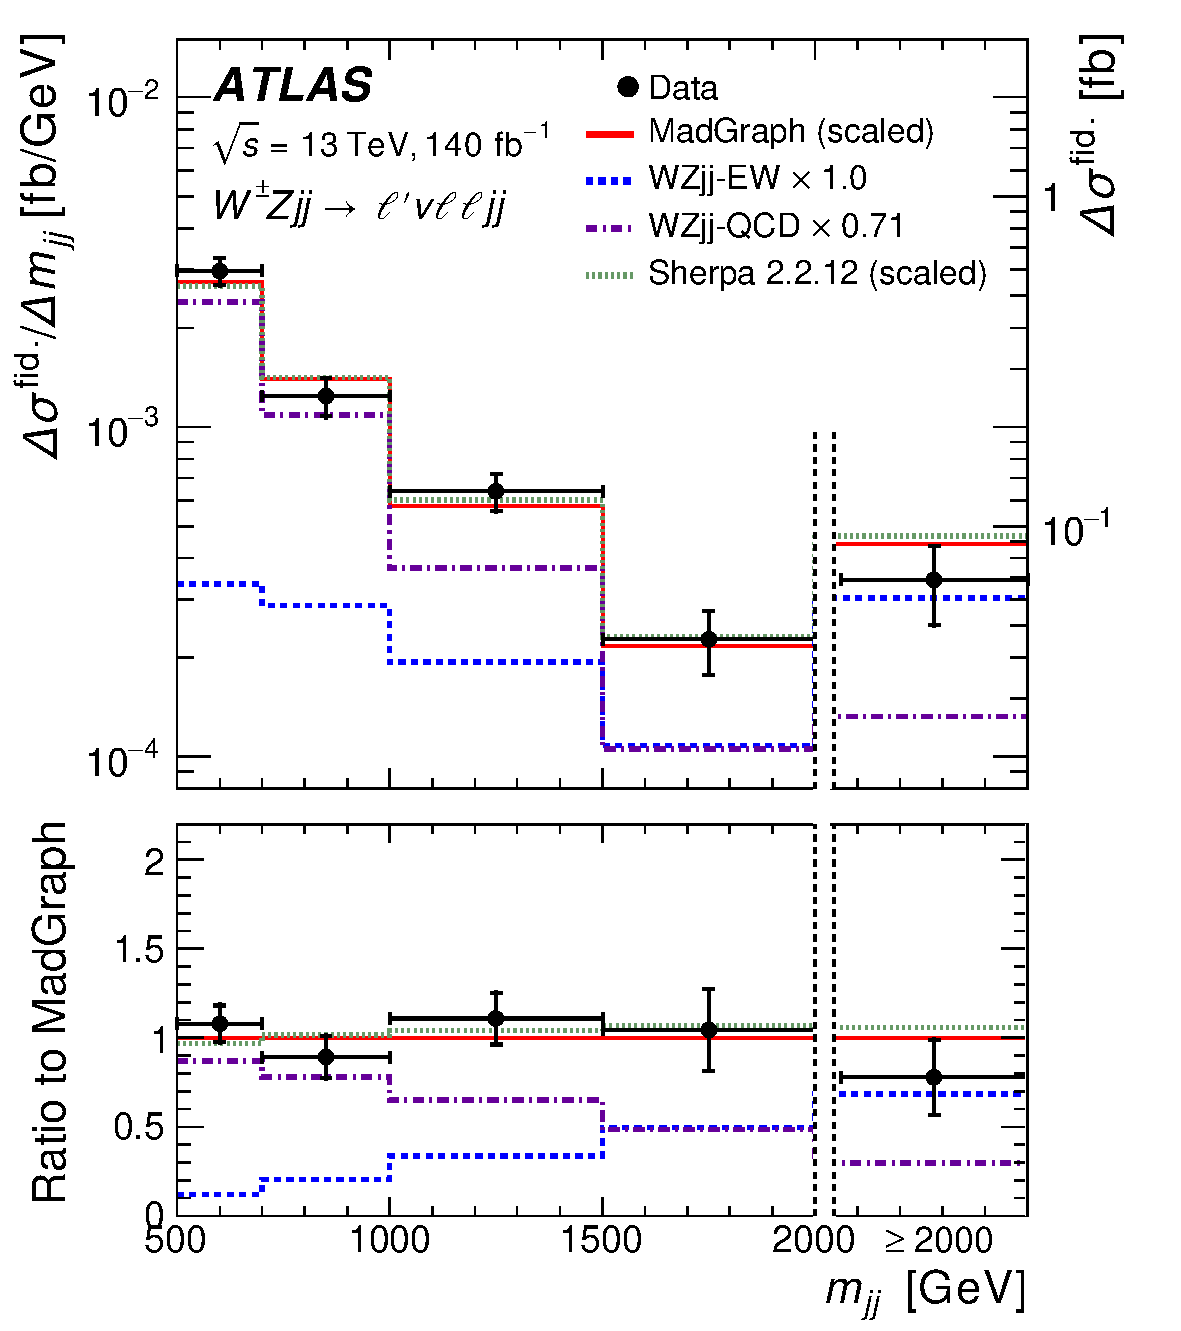
\includegraphics[width=0.45\textwidth]{Immagini/fig_08c.pdf}}
\subfloat[]{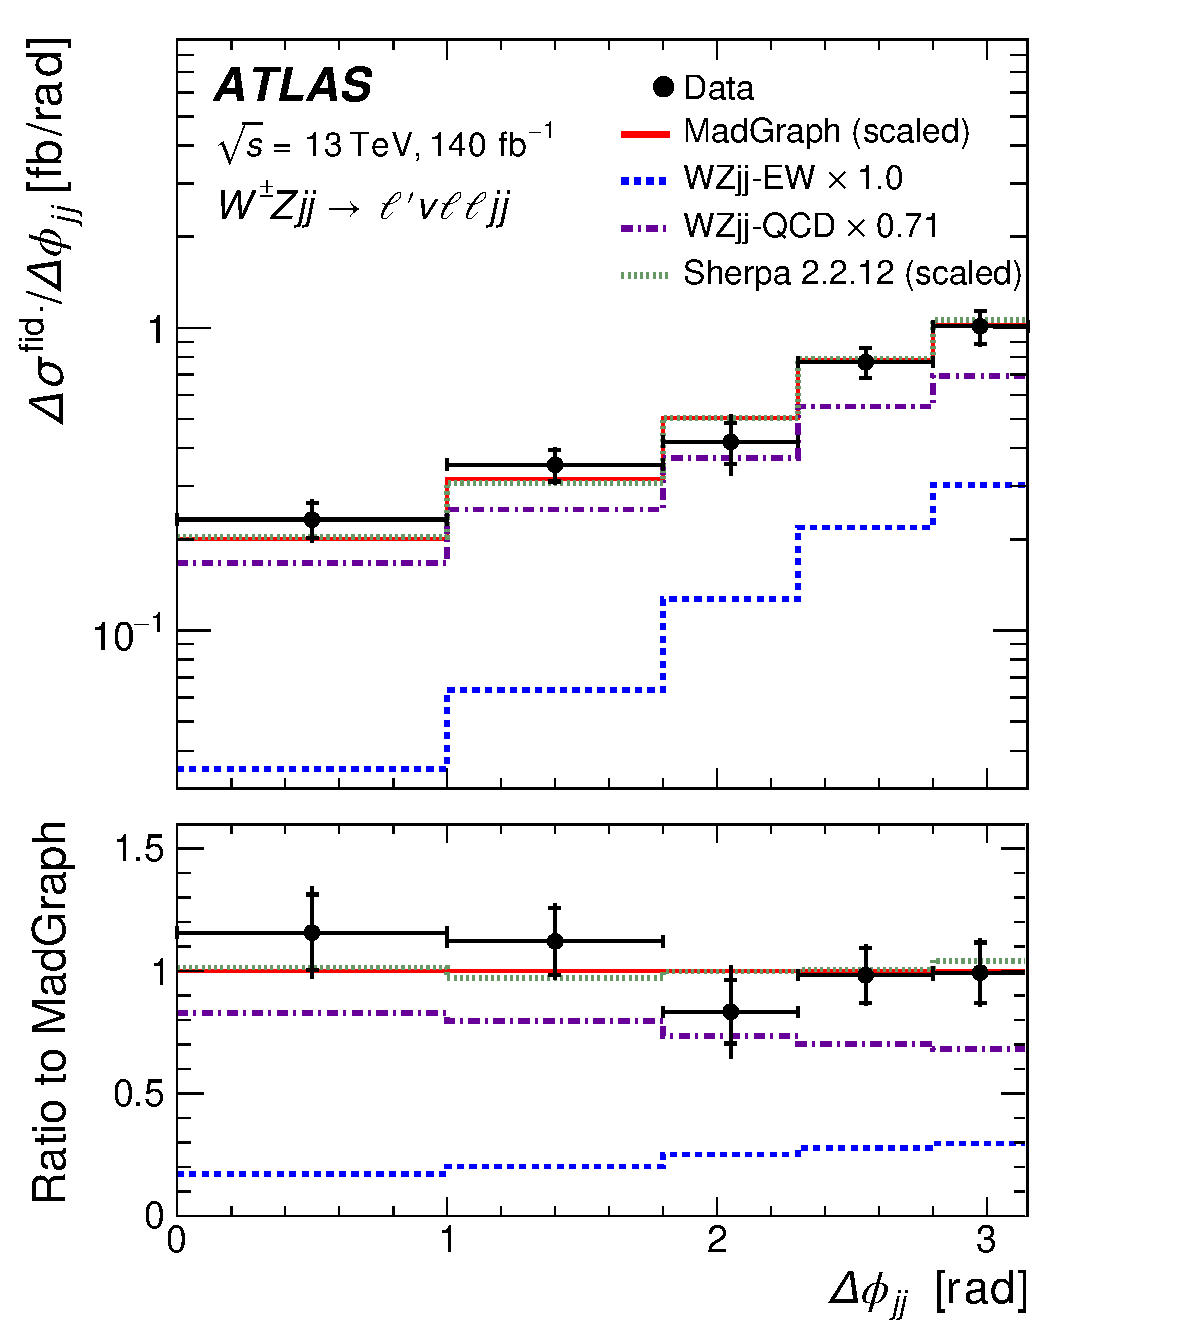
\includegraphics[width=0.45\textwidth]{Immagini/fig_08d.pdf}}
\caption{Sezione d'urto differenziale inclusiva di \wzjj\ misurata nello spazio delle fasi fiduciale del VBS in funzione di: (a) molteplicità esclusiva di jet con $p_T > 40\,\unit{GeV}$ ($N_{\text{jet}}^{40}$), (b) differenza assoluta in rapidità tra i due jet di \textit{tagging} ($\Delta y_{jj}$), (c) massa invariante dei jet di \textit{tagging} (\mjj), e (d) angolo azimutale tra i due jet di \textit{tagging} ($\Delta\phi_{jj}$). Le definizioni delle barre di errore, delle linee e dei pannelli inferiori seguono la convenzione di Figura~\ref{fig:diffXSection:SptL_dPhiWZ}.}
\label{fig:diffXSection:dYjj_mjj}
\end{figure}


\begin{figure}[htbp]
\centering
\subfloat[]{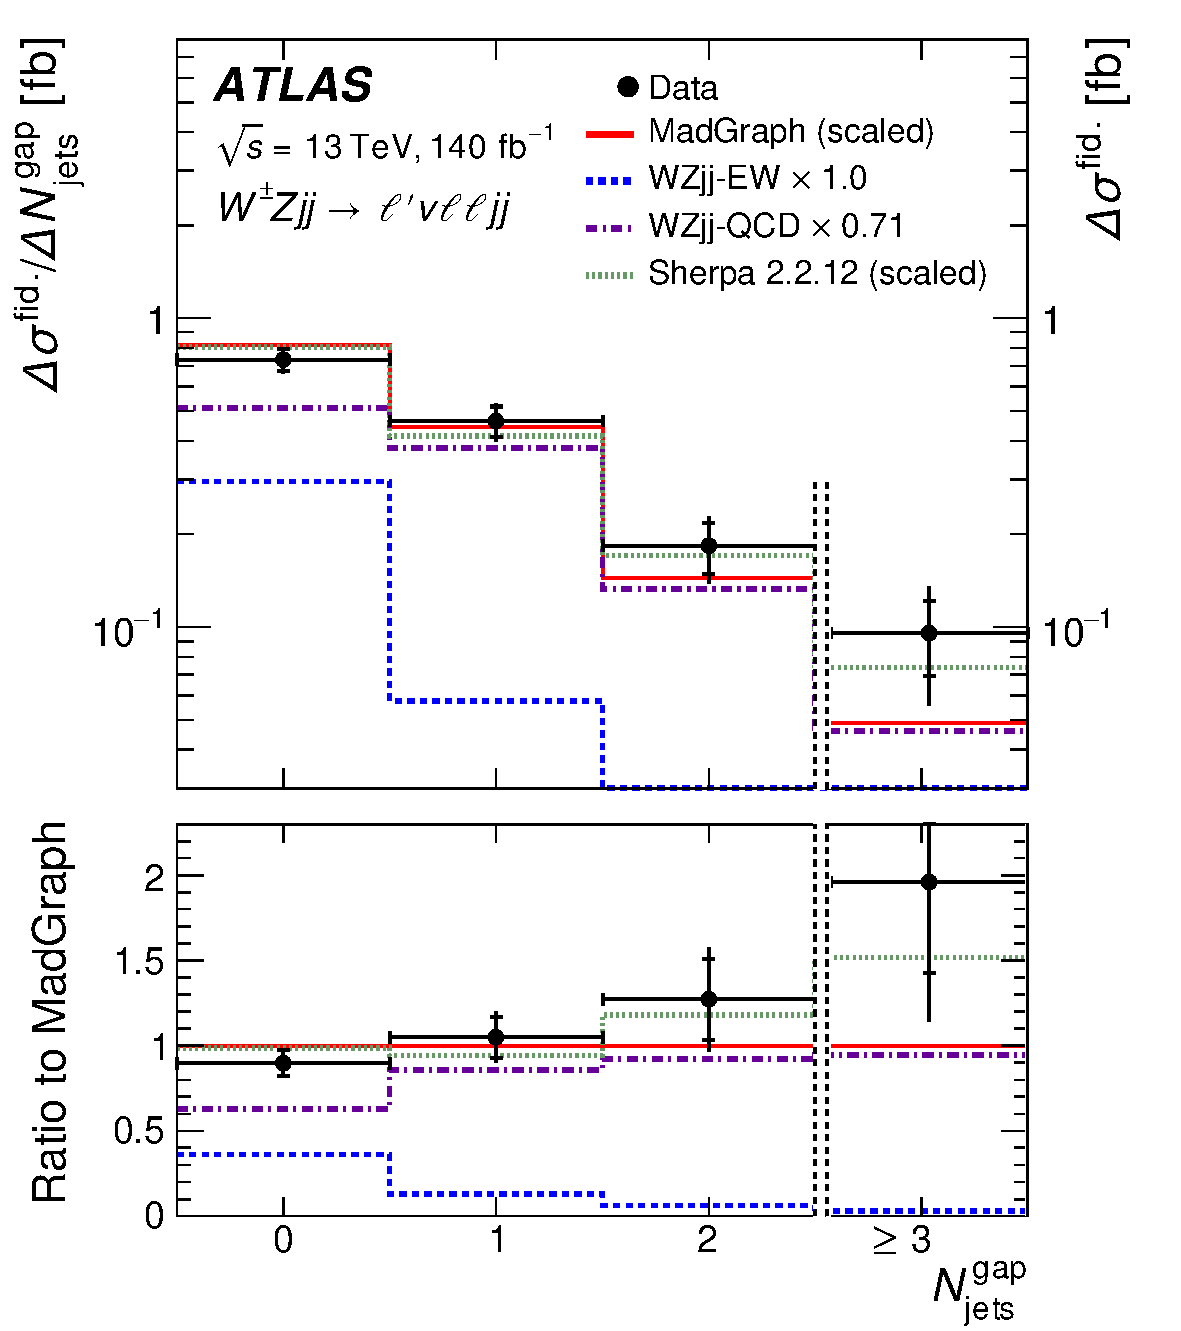
\includegraphics[width=0.45\textwidth]{Immagini/fig_09a.pdf}}
\subfloat[]{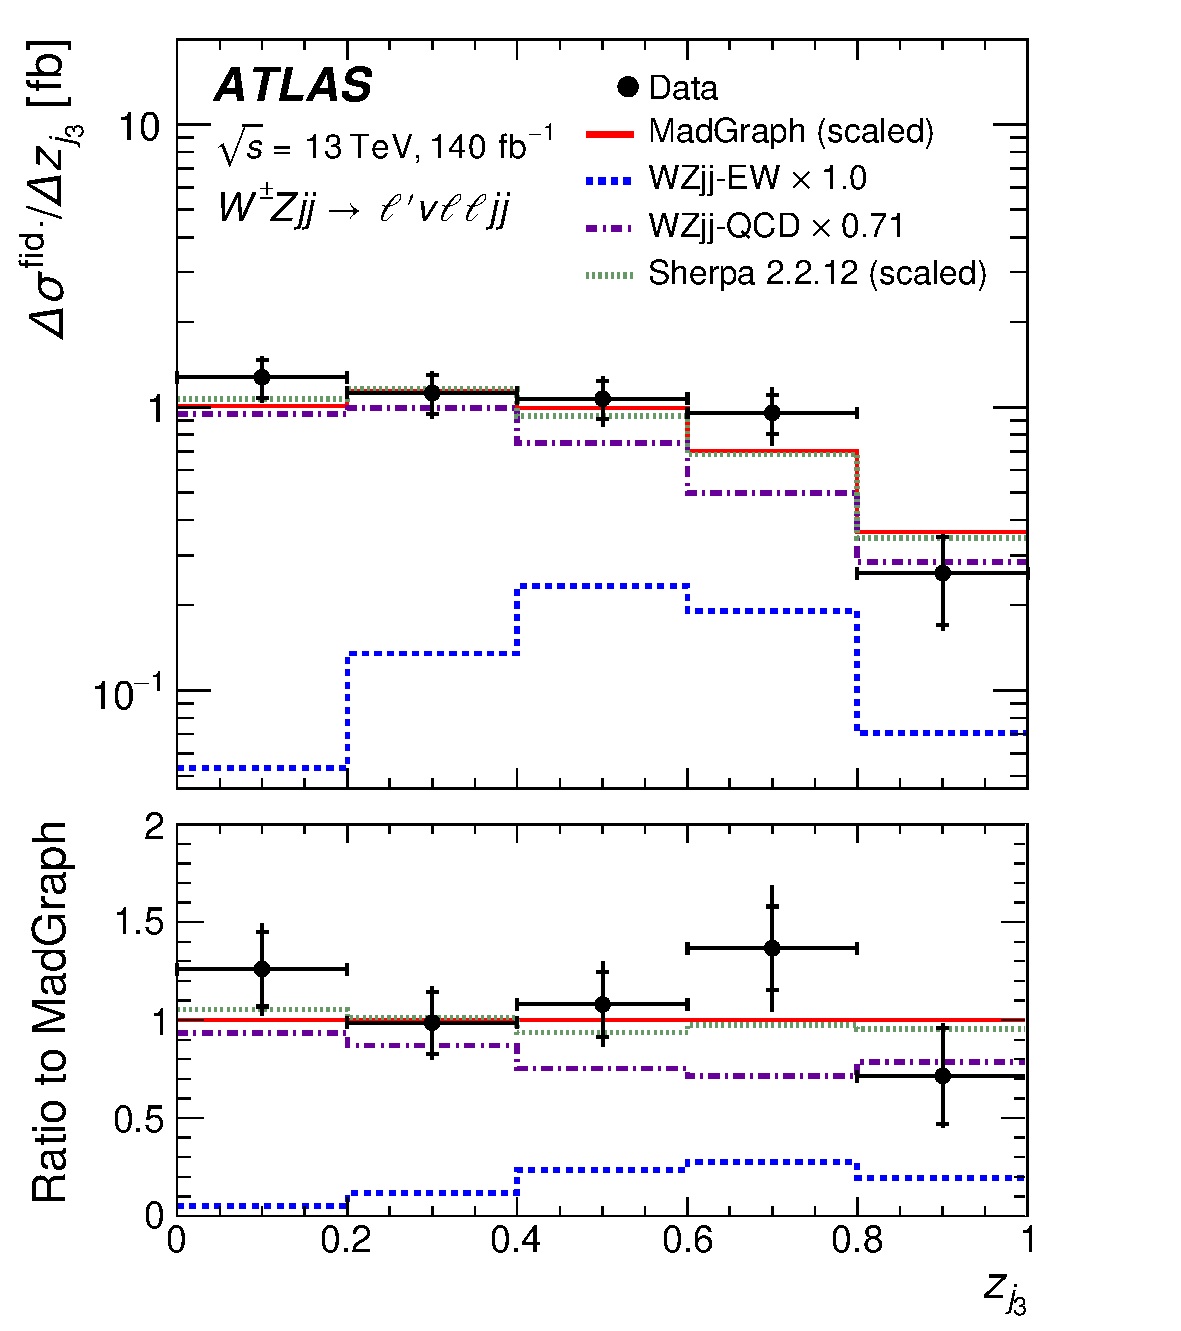
\includegraphics[width=0.45\textwidth]{Immagini/fig_09b.pdf}}
\caption{Sezione d'urto differenziale inclusiva di \wzjj\ misurata nello spazio delle fasi fiduciale del VBS in funzione di: (a) $N_{\text{jet}}^{\text{gap}}$ (molteplicità esclusiva di jet con $p_T > 25\,\unit{GeV}$ nel gap di pseudorapidità tra i due jet di \textit{tagging}) e (b) $\zeta_{j3}$ (variabile di Zeppenfeld per il terzo jet). Le definizioni delle barre di errore, delle linee e dei pannelli inferiori seguono la convenzione di Figura~\ref{fig:diffXSection:SptL_dPhiWZ}.}
\label{fig:diffXSection:3rdjet}
\end{figure}


\begin{figure}[htbp]
\centering
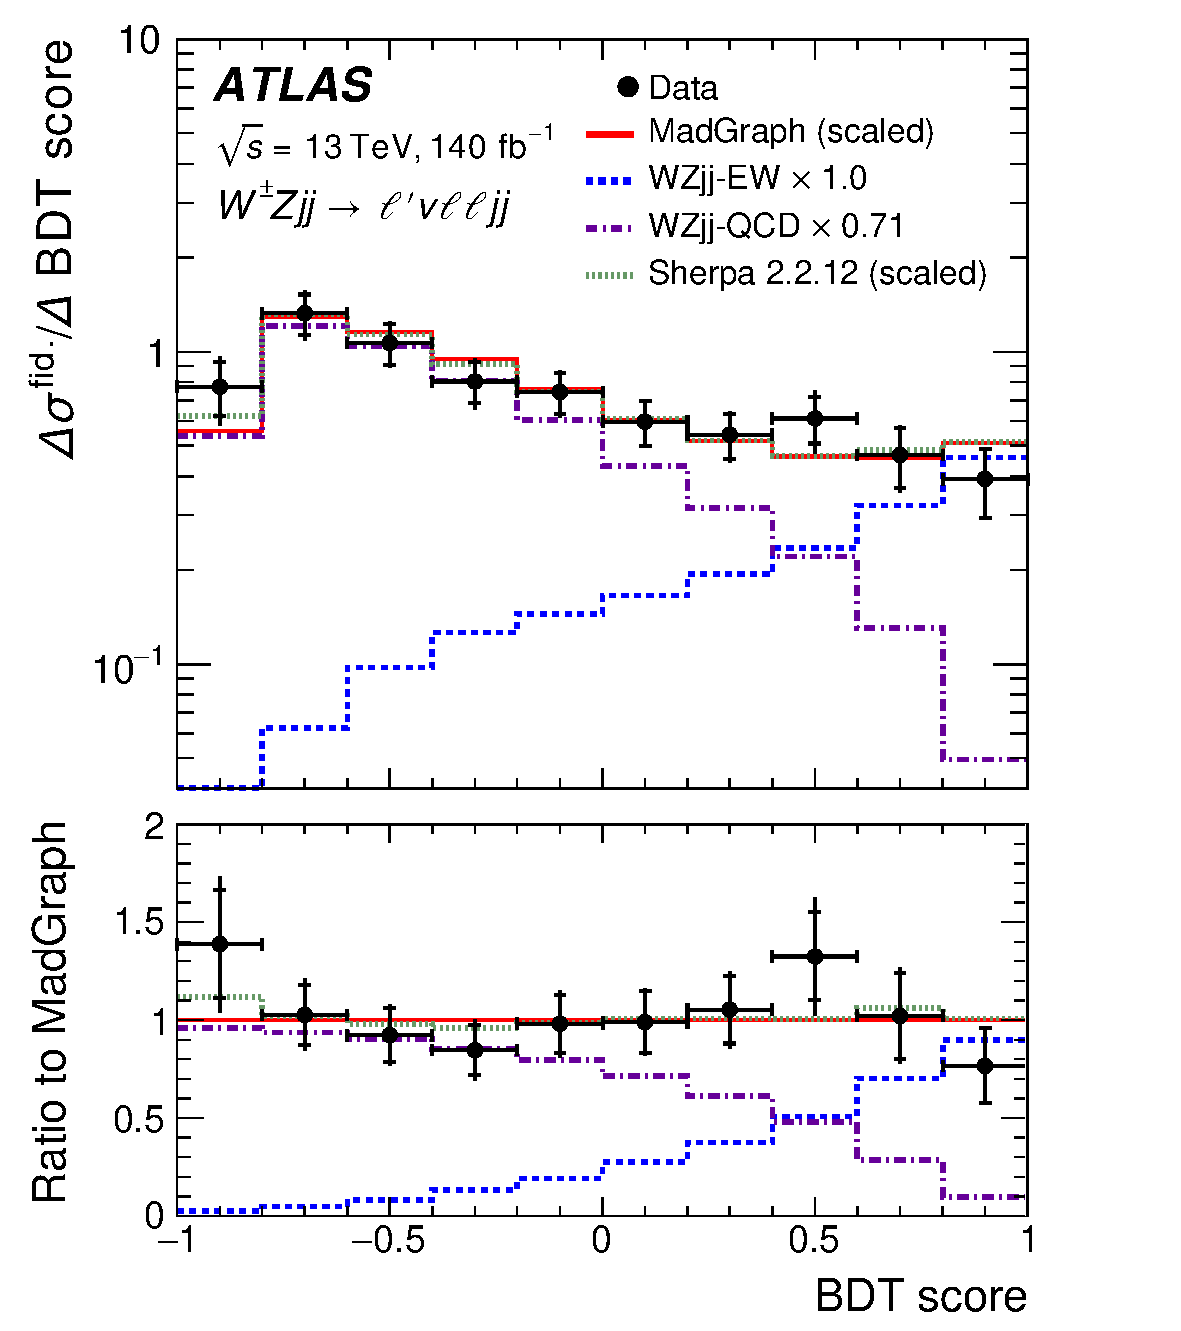
\includegraphics[width=0.45\textwidth]{Immagini/fig_10.pdf}
\caption{Sezione d'urto differenziale inclusiva di \wzjj\ misurata nello spazio delle fasi fiduciale del VBS in funzione dello \textit{score} del BDT. Le barre di errore interne ed esterne sui punti dati rappresentano rispettivamente le incertezze statistiche e totali. I risultati sono confrontati con la combinazione dei contributi teorici riscalati.}
\label{fig:diffXSection:BDT}
\end{figure}


Le misure delle sezioni d'urto differenziali inclusive di \wzjj\ sono eseguite in funzione di tre variabili cinematiche particolarmente sensibili a eventuali anomalie negli accoppiamenti quartici dei bosoni di gauge (aQGC): la somma scalare dei momenti trasversi dei tre leptoni carichi associati ai bosoni $W$ e $Z$ ($\sum p_T^\ell$), la differenza di angolo azimutale $\Delta\phi(W,Z)$ tra le direzioni del $W$ e del $Z$, e la massa trasversa del sistema $WZ$ (\mtwz). Queste distribuzioni sono presentate nella Figura \ref{fig:diffXSection:SptL_dPhiWZ}.

Le misure vengono effettuate anche in funzione di variabili legate alla cinematica dei jet: la molteplicità esclusiva di jet con $p_T > 40\,\unit{GeV}$ ($N_{\text{jet}}^{40}$), la differenza assoluta in rapidità tra i due jet di \textit{tagging} ($\Delta y_{jj}$), la massa invariante dei jet di \textit{tagging} (\mjj), la molteplicità esclusiva di jet con $p_T > 25\,\unit{GeV}$ nel gap di pseudorapidità $\eta$ tra i due jet di \textit{tagging} ($N_{\text{jet}}^{\text{gap}}$), e l'angolo azimutale tra i due jet di \textit{tagging} ($\Delta\phi_{jj}$), mostrati in Figura \ref{fig:diffXSection:dYjj_mjj}.

Le misure relative all'attività dei jet nella regione di gap tra i due jet di \textit{tagging} vengono eseguite anche sfruttando il sotto-campione di eventi nella SR in cui è presente un terzo jet con $p_T > 25\,\unit{GeV}$. La molteplicità esclusiva $N_{\text{jet}}^{\text{gap}}$ per jet con $p_T > 25\,\unit{GeV}$ nel gap in $\eta$ e la variabile di Zeppenfeld $\zeta_{j3}$ per il terzo jet sono presentate nella Figura \ref{fig:diffXSection:3rdjet}. La variabile $\zeta_{j3}$ è definita come:
\begin{equation}
\zeta_{j3} = \left| \frac{y_{j_3} - \frac{1}{2}\left(y_{j_1} + y_{j_2}\right)}{y_{j_1} - y_{j_2}} \right|
\end{equation}
dove $y_{j_i}$ rappresenta la rapidità del rispettivo jet $i$.

Infine, viene eseguita una misura differenziale della sezione d'urto di produzione inclusiva di \wzjj\ in funzione dello \textit{score} del BDT, presentata nella Figura \ref{fig:diffXSection:BDT}. La predizione dello \textit{score} del BDT a livello di particella generata viene valutata utilizzando lo stesso BDT addestrato a livello del rivelatore, ma calcolato a partire dalle osservabili di input particellari.

Le incertezze totali in queste misure differenziali sono dominate dall'errore statistico dei dati. I risultati differenziali sono confrontati con le predizioni di \textsc{MGPy8}, dopo aver riscalato le componenti separate \wzjjqcd\ e \wzjjew\ alle sezioni d'urto inclusive $\sigma_{\text{strong}}$ e $\sigma_{\text{EW}}$ ottenute dal fit di massima verosimiglianza sui dati. Gli effetti di interferenza tra i processi sono incorporati nella predizione della componente forte. Le misure sono confrontate anche con le predizioni indipendenti del generatore \textsc{Sherpa}~2.2.12.
\newpage
\section{Limiti sugli accoppiamenti di gauge quartici anomali}
\label{sec:EFT_limits}

La produzione \wzjjew\ può essere sensibile a effetti oltre il Modello Standard (SM) che influenzano le interazioni quartiche dei bosoni deboli. Gli eventi \wzjj\ misurati sono quindi utilizzati per cercare accoppiamenti di gauge quartici anomali (aQGC) utilizzando il formalismo delle teorie di campo efficaci (EFT). In questo modello, la Lagrangiana del Modello Standard $\mathcal{L}_{\mathrm{SM}}$ viene estesa in una Lagrangiana efficace $\mathcal{L}_{\mathrm{eff}}$ aggiungendo operatori di ordine superiore e i loro rispettivi coefficienti di Wilson come segue:

\begin{equation} \label{eq:EFT_Lagrangian}
\mathcal{L}_{\mathrm{eff}} = \mathcal{L}_{\mathrm{SM}}+\sum_i \frac{f_i^{(6)}}{\Lambda_i^2} O_i^{(6)}+\sum_j \frac{f_j^{(8)}}{\Lambda_j^4} O_j^{(8)}+\ldots \; ,
\end{equation}

dove $O_{i,j}^{(6),(8)}$ sono rispettivamente operatori di dimensione-6 e di dimensione-8, i quali coinvolgono i campi del Modello Standard con i rispettivi accoppiamenti adimensionali $f_i^{(6)}$ e $f_j^{(8)}$, mentre $\Lambda$ rappresenta la scala di energia dei nuovi processi. In questo studio vengono considerati solo operatori di dimensione-8 e si assume che tutti gli accoppiamenti di dimensione-6, i quali influenzano i vertici di gauge tripli, siano pari a zero. Gli accoppiamenti di dimensione-6 sono infatti già vincolati in maniera stringente da altri processi, in particolare dalla produzione inclusiva di dibosoni. L'effetto degli operatori di dimensione-6 nei processi VBS è di per sé di grande interesse, ma non viene studiato in questa sede. 

Vengono presi in considerazione nove operatori indipendenti di dimensione-8 che conservano la parità e la coniugazione di carica. Gli operatori $O_{\mathrm{S}0,\, 1,\, 2}$ sono costruiti a partire dalla derivata covariante del doppietto di Higgs. Gli operatori $O_{\mathrm{T}0,\, 1,\, 2}$ sono costruiti a partire dai campi di gauge di $\mathrm{SU}_{\mathrm{L}}(2)$. Gli operatori misti $O_{\mathrm{M}0,\, 1,\, 7}$ coinvolgono sia i campi di gauge di $\mathrm{SU}_{\mathrm{L}}(2)$ sia il doppietto di Higgs. Poiché gli operatori $O_{\mathrm{S}0}$ e $O_{\mathrm{S}2}$ sono l'uno il coniugato hermitiano dell'altro, essi vengono fatti variare simultaneamente, assumendo coefficienti di identico valore $f_{\mathrm{S}0} = f_{\mathrm{S}2} = f_{\mathrm{S}02}$.

L'ampiezza di scattering al quadrato predetta dalla teoria di campo efficace per la produzione \wzjj\ può essere scritta come:

\begin{equation}
\left| A_{\mathrm{SM}}+\sum_i c_i A_i \right|^2 = {\left| A_{\mathrm{SM}} \right| }^2 + \sum_i c_i \, 2 \operatorname{Re}(A^*_{\mathrm{SM}}A_i)+ \sum_i c_i^2 |A_i|^2 +\sum_{ij,i\neq j} c_i c_j \, 2 \operatorname{Re}(A_{i} A^*_{j}) \; ,
\label{eq:EFT}
\end{equation}

dove $c_i = f_j^{(8)} / \Lambda^4$, $A_{\mathrm{SM}}$ è l'ampiezza di scattering del Modello Standard, $\sum_i c_i \, 2 \operatorname{Re}(A^*_{\mathrm{SM}} A_i)$ è l'ampiezza del termine di interferenza tra il Modello Standard e gli operatori di dimensione-8, $\sum_i {c_i}^2 |A_i|^2$ è il contributo puramente di dimensione-8, e $\sum_{ij,i\neq j} c_i c_j 2 \operatorname{Re}(A_i A^*_j)$ rappresenta l'ampiezza di interferenza incrociata tra due operatori di dimensione-8 (\textit{cross terms}).
Questi diversi termini sono simulati separatamente utilizzando \textsc{MadGraph5\_aMC@NLO}~2.6.5 interfacciato con \textsc{Pythia}~8.240, fornendo campioni MC indipendenti. Vengono utilizzati gli stessi set di PDF e la medesima modellizzazione del \textit{parton shower} (PS) impiegati per gli eventi \wzjj\ del Modello Standard e dettagliati in precedenza. Gli eventi generati corrispondenti a un dato valore del coefficiente EFT $c_i$ (oppure alla coppia $c_i$ e $c_j$ per i termini incrociati) si ottengono moltiplicando i rispettivi campioni MC per il valore del coefficiente e sommandoli tra loro.

Poiché la presenza di contributi aQGC non nulli tende ad aumentare la sezione d'urto di produzione degli eventi \wzjjew\ per grandi valori della massa invariante dibosonica, per la ricerca dei contributi EFT di dimensione-8 si utilizza una combinazione bidimensionale composta dallo \textit{score} del BDT (che isola il segnale \wzjjew\ dal fondo \wzjjqcd) e dalla massa trasversa \mtwz. Si utilizzano quattro \textit{bin} per lo \textit{score} del BDT ($[-1, -0.25, 0.17, 0.72, 1]$) e cinque \textit{bin} per \mtwz\ ($[0, 400, 750, 1050, 1350, \infty]\,\unit{GeV}$), disposti in un istogramma unidimensionale costituito da 20 \textit{bin} statisticamente indipendenti, come illustrato in Figura~\ref{fig:2D_EFTTemplate}. I bordi dei \textit{bin} sono stati ottimizzati per ottenere i limiti attesi più stringenti in assenza di un \textit{cut-off} di unitarizzazione.
Questa distribuzione viene utilizzata per definire una funzione di verosimiglianza estesa, includendovi le stesse regioni di controllo descritte in precedenza. Le incertezze sperimentali e teoriche sono incorporate nel fit come parametri di disturbo (\textit{nuisance parameters}) vincolati in modo gaussiano. 
Viene costruita una statistica di test basata sul rapporto delle verosimiglianze profilate (\textit{profile-likelihood ratio}) per stimare gli intervalli di confidenza per un dato $c_i$. Per ogni singolo coefficiente $c_i$, o per ogni coppia $(c_i, c_j)$ nel caso dei limiti bidimensionali, si esegue un fit di massima verosimiglianza sui dati ponendo temporaneamente a zero tutti gli altri coefficienti.

\begin{figure}[htbp]
\centering
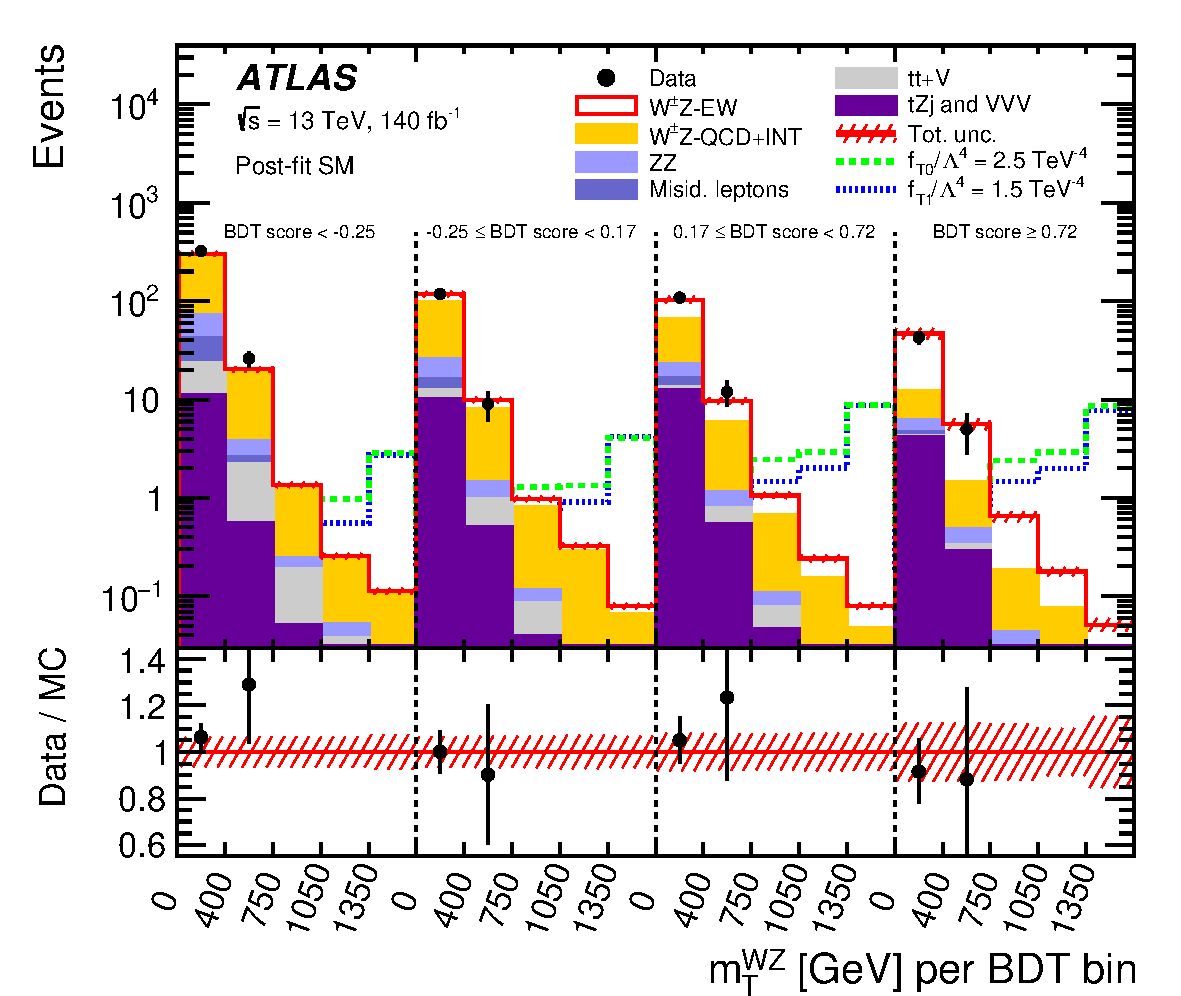
\includegraphics[scale=0.6]{Immagini/fig_11.pdf}
\caption{Distribuzione unidimensionale a livello di rivelatore derivante dalla combinazione bidimensionale delle variabili \textit{score} del BDT e \mtwz, utilizzata per estrarre i limiti sui coefficienti EFT. Sono mostrate le rese degli eventi previste dal fit eseguito sui dati assumendo la validità del solo Modello Standard. La banda di incertezza attorno all'attesa MC include le incertezze sistematiche totali ottenute dal fit. Vengono inoltre mostrati i contributi degli operatori $O_{\mathrm{T}0}$ e $O_{\mathrm{T}1}$ per valori puramente illustrativi dei rispettivi coefficienti di Wilson.}
\label{fig:2D_EFTTemplate}
\end{figure}

\begin{table}[htbp]
\caption{Intervalli di confidenza attesi e osservati al $95\%$ CL sui coefficienti di Wilson dei vari operatori di dimensione-8, senza l'applicazione di procedure di unitarizzazione. La notazione $\mathrm{S}02$ indica che ai coefficienti associati agli operatori $O_{\mathrm{S}0}$ e $O_{\mathrm{S}2}$ viene assegnato il medesimo valore numerico.}
\label{tab:limitsNoCl}
\centering
\renewcommand{\arraystretch}{1.3}
\begin{tabular}{c c c}
\hline
\textbf{Coefficiente} & \textbf{Atteso [$\unit{TeV}^{-4}$]} & \textbf{Osservato [$\unit{TeV}^{-4}$]} \\
\hline
\hline
$f_{\mathrm{T}0}/{\Lambda}^4$ & $[-0.80, 0.80]$ & $[-0.57, 0.56]$ \\
$f_{\mathrm{T}1}/{\Lambda}^4$ & $[-0.52, 0.49]$ & $[-0.39, 0.35]$ \\
$f_{\mathrm{T}2}/{\Lambda}^4$ & $[-1.6, 1.4]$ & $[-1.2, 1.0]$ \\
$f_{\mathrm{M}0}/{\Lambda}^4$ & $[-8.3, 8.3]$ & $[-5.8, 5.6]$ \\
$f_{\mathrm{M}1}/{\Lambda}^4$ & $[-12.3, 12.2]$ & $[-8.6, 8.5]$ \\
$f_{\mathrm{M}7}/{\Lambda}^4$ & $[-16.2, 16.2]$ & $[-11.3, 11.3]$ \\
$f_{\mathrm{S}02}/{\Lambda}^4$ & $[-14.2, 14.2]$ & $[-10.4, 10.4]$ \\
$f_{\mathrm{S}1}/{\Lambda}^4$ & $[-42, 41]$ & $[-30, 30]$ \\
\hline
\end{tabular}
\end{table}

Non si osserva alcuna deviazione rispetto alle previsioni del Modello Standard; i limiti inferiori e superiori attesi e osservati al $95\%$ di livello di confidenza (CL) per i coefficienti di Wilson considerati sono riportati nella Tabella~\ref{tab:limitsNoCl}. I coefficienti associati agli operatori $O_{\mathrm{T}0}$ e $O_{\mathrm{T}1}$ risultano essere i più stringenti. Tali limiti sono dominati dal contributo puramente di dimensione-8 presentato nell'Equazione~(\ref{eq:EFT}). Questi risultati sono simili a quelli ottenuti dall'esperimento CMS, anch'esso analizzando i canali di decadimento leptonici negli eventi \wzjj~\cite{CMS:2020gfh}. Sono stati inoltre ricavati i limiti bidimensionali al $95\%$ CL sulla coppia di operatori $O_{\mathrm{T}0}$ e $O_{\mathrm{T}1}$, mostrati nella Figura~\ref{fig:2D_exp_plots_reco}. Per ottenere questi risultati non è stata impiegata alcuna procedura di unitarizzazione.

\begin{figure}[htbp]
\centering
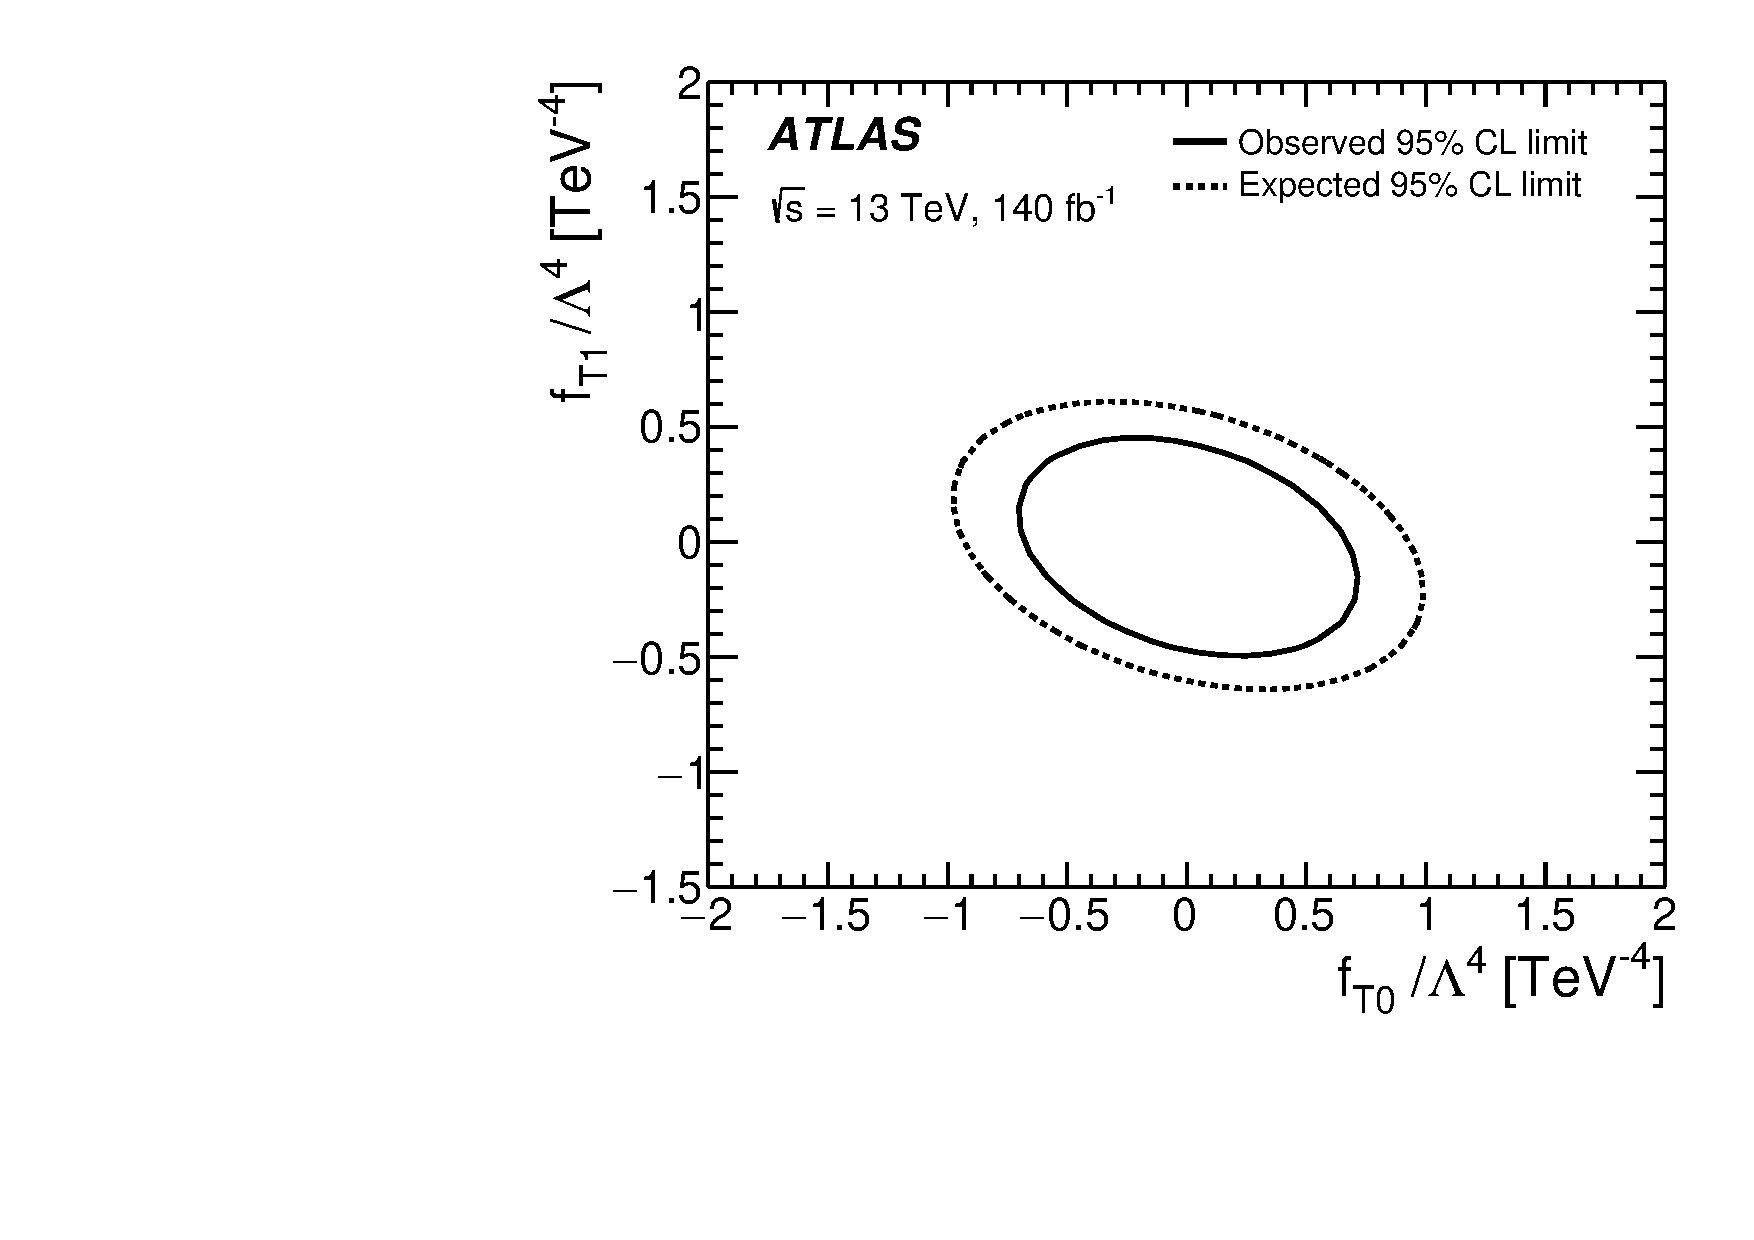
\includegraphics[scale=0.4]{Immagini/fig_12.pdf}
\caption{Intervalli di confidenza bidimensionali al $95\%$ CL attesi (linea tratteggiata) e osservati (linea continua) per i coefficienti di Wilson associati alla coppia di operatori $O_{\mathrm{T}0}$ e $O_{\mathrm{T}1}$, senza l'uso di \textit{cut-off} di unitarizzazione.}
\label{fig:2D_exp_plots_reco}
\end{figure}

Il framework EFT non rappresenta un modello fisico completo, e la presenza di operatori di dimensione-8 non nulli viola matematicamente l'unitarietà a livello albero qualora l'energia sia sufficientemente elevata. Limiti fisicamente più accurati possono essere ottenuti sopprimendo il contributo EFT al di sopra del limite di unitarietà e mantenendo attiva la sola predizione del Modello Standard per tutte le masse invarianti del sistema $WZ$, anche superata tale soglia. I limiti di unitarietà calcolati dalla Ref.~\cite{Almeida:2020ylr} vengono adoperati assumendo l'esistenza di un solo coefficiente di Wilson non nullo alla volta. Questi limiti di unitarietà sono presentati nella Figura~\ref{fig:clipping_T} per i coefficienti $f_{\mathrm{T}0}$ e $f_{\mathrm{T}1}$, affiancati dall'evoluzione degli intervalli attesi e osservati al $95\%$ CL tracciati in funzione della scala di \textit{cut-off} $m_{WZ}$ impiegata nella procedura di unitarizzazione.

La Tabella~\ref{tab:limitsWithCl} presenta i singoli intervalli di esclusione al $95\%$ CL per ciascun coefficiente di Wilson, ottenuti imponendo un \textit{cut-off} di unitarizzazione in corrispondenza del limite teorico. Per l'operatore $O_{\mathrm{S}1}$ non è stato individuato alcun incrocio con la curva del limite di unitarietà nella regione scansionata oltre i $600\,\unit{GeV}$, pertanto per esso non viene riportato alcun limite.

\begin{figure}[htbp]
\centering
\subfloat[]{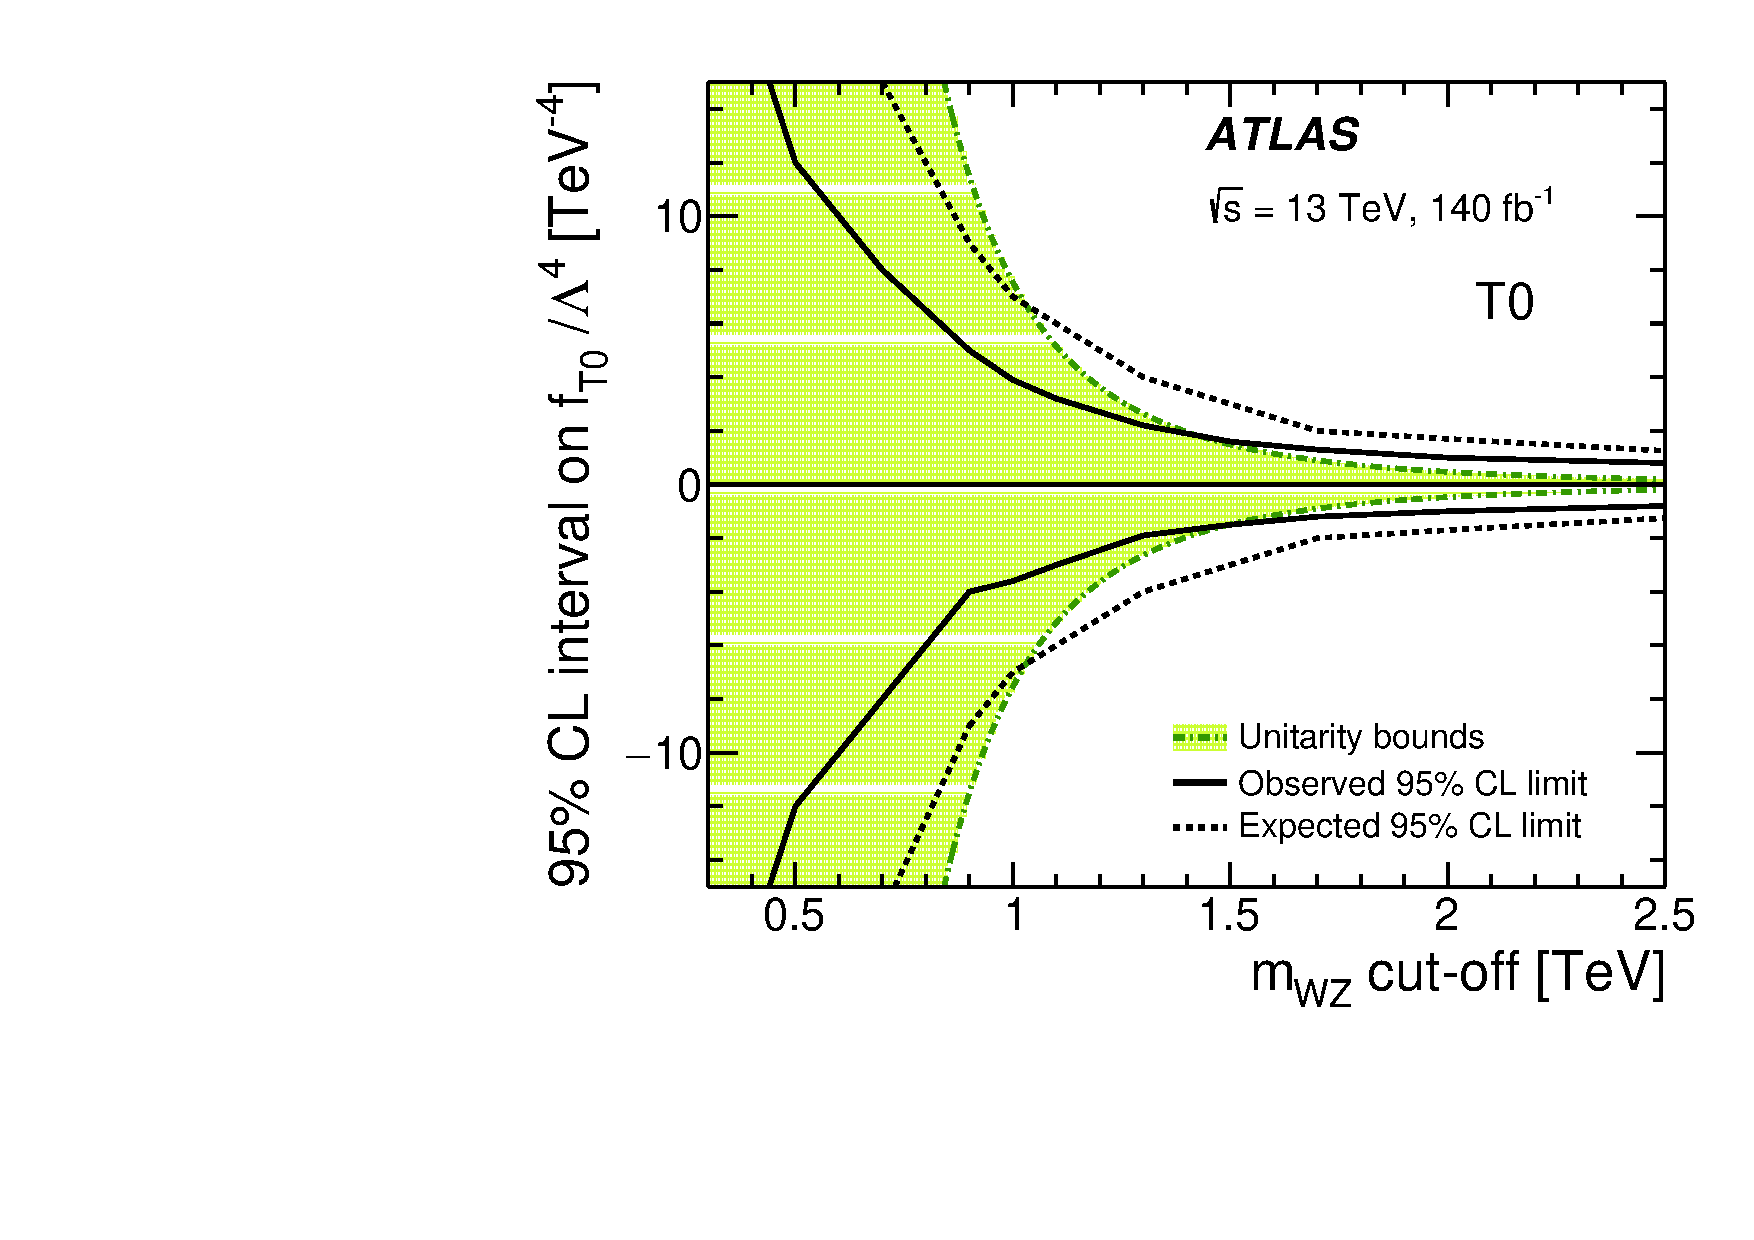
\includegraphics[scale=0.4]{Immagini/fig_13a.pdf}}
\subfloat[]{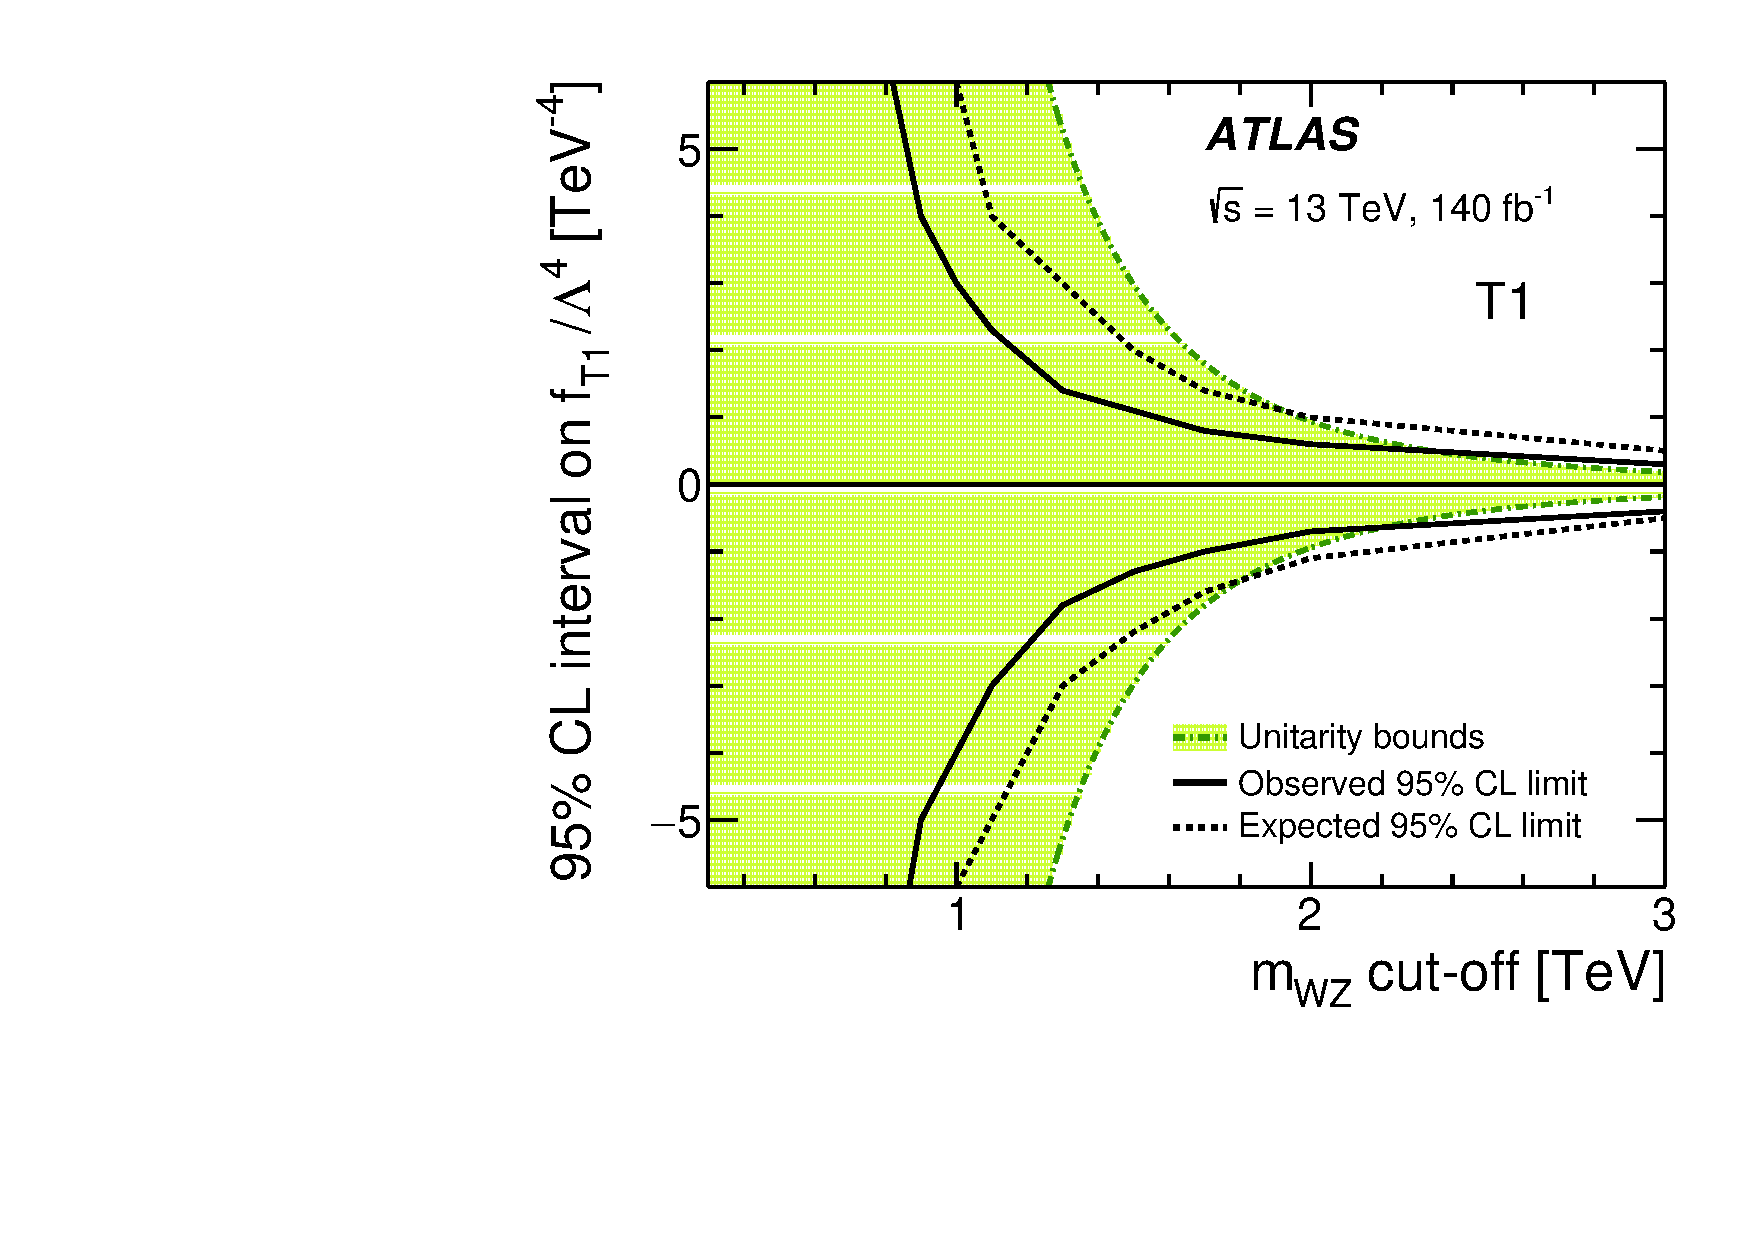
\includegraphics[scale=0.4]{Immagini/fig_13b.pdf}}
\caption{Evoluzione in funzione della scala di \textit{cut-off} dei limiti individuali attesi (linee tratteggiate) e osservati (linee continue) al $95\%$ CL sui coefficienti di Wilson per gli operatori (a) $O_{\mathrm{T}0}$ e (b) $O_{\mathrm{T}1}$. L'area ombreggiata rappresenta la regione consentita dall'unitarietà. I limiti di unitarietà (linee tratto-punto) per ciascun operatore sono calcolati assumendo un solo coefficiente non nullo, secondo la Ref.~\cite{Almeida:2020ylr}.}
\label{fig:clipping_T}
\end{figure}

\begin{table}[htbp]
\caption{Intervalli di confidenza attesi e osservati al $95\%$ CL sui coefficienti di Wilson dei vari operatori di dimensione-8, ottenuti impostando un \textit{cut-off} di unitarizzazione esattamente in corrispondenza del limite unitario teorico (ossia nel punto di incrocio tra il limite sperimentale e il limite teorico). La notazione $\mathrm{S}02$ indica che i coefficienti associati agli operatori $O_{\mathrm{S}0}$ e $O_{\mathrm{S}2}$ assumono lo stesso valore.}
\label{tab:limitsWithCl}
\centering
\renewcommand{\arraystretch}{1.3}
\begin{tabular}{c c c}
\hline
\textbf{Coefficiente} & \textbf{Atteso [$\unit{TeV}^{-4}$]} & \textbf{Osservato [$\unit{TeV}^{-4}$]} \\
\hline
\hline
$f_{\mathrm{T}0}/{\Lambda}^4$ & $[-7.0, 7.0]$ & $[-1.5, 1.6]$ \\
$f_{\mathrm{T}1}/{\Lambda}^4$ & $[-1.1, 1.0]$ & $[-0.7, 0.6]$ \\
$f_{\mathrm{T}2}/{\Lambda}^4$ & $[-12, 6]$ & $[-2.4, 1.8]$ \\
$f_{\mathrm{M}0}/{\Lambda}^4$ & $[-60, 60]$ & $[-12, 12]$ \\
$f_{\mathrm{M}1}/{\Lambda}^4$ & $[-32, 32]$ & $[-15, 15]$ \\
$f_{\mathrm{M}7}/{\Lambda}^4$ & $[-30, 30]$ & $[-15, 15]$ \\
$f_{\mathrm{S}02}/{\Lambda}^4$ & $[-41, 41]$ & $[-18, 18]$ \\
$f_{\mathrm{S}1}/{\Lambda}^4$ & --- & --- \\
\hline
\end{tabular}
\end{table}

\section{Conclusioni}
\label{sec:conclusion}

In questo articolo vengono presentate le misure delle sezioni d'urto integrate e differenziali della produzione elettrodebole di una coppia \wz\ in associazione a due jet, e della sua sezione d'urto di produzione in collisioni $pp$ a $\sqrt{s} = 13\,\unit{TeV}$ all'LHC. I dati sono stati raccolti attraverso il rivelatore ATLAS e corrispondono a una luminosità integrata di $140\,\unit{fb}^{-1}$. Le misure sfruttano i canali di decadimento leptonico dei bosoni di gauge in elettroni o muoni e sono eseguite in uno spazio delle fasi fiduciale che modella l'accettanza del rivelatore per massimizzare la sensibilità nei confronti dei processi di produzione elettrodebole \wzjj.

Le sezioni d'urto fiduciali integrate misurate per un singolo canale di decadimento leptonico per la produzione \wzjj\ elettrodebole e inclusiva risultano essere, rispettivamente, $\sigma_{W^\pm Zjj\mathrm{-EW} \rightarrow \ell' \nu \ell \ell jj} = 0.368 \pm 0.037\,\text{(stat.)} \pm 0.059\,\text{(syst.)} \pm 0.003\,\text{(lumi.)}\,\unit{fb}$ e $\sigma_{W^\pm Zjj \rightarrow \ell' \nu \ell \ell jj} = 1.462 \pm 0.063\,\text{(stat.)} \pm 0.118\,\text{(syst.)} \pm 0.012\,\text{(lumi.)}\,\unit{fb}$. A oggi, questa rappresenta la misurazione più precisa esistente della sezione d'urto di produzione \wzjjew. La sezione d'urto di produzione elettrodebole \wzjj\ risulta in accordo con le previsioni del Modello Standard calcolate al LO pari a $0.37 \pm 0.03\,\unit{fb}$, ricavate tramite il generatore di eventi MC \textsc{MadGraph5\_aMC@NLO}+\textsc{Pythia8} (\textsc{MGPy8}). Tuttavia, la sezione d'urto inclusiva per la produzione \wzjj\ si è rivelata inferiore alle previsioni del Modello Standard fornite dal generatore \textsc{MGPy8} ($1.91 \pm 0.17\,\unit{fb}$). Il motivo di tale discostamento risiede nel fatto che la sezione d'urto integrata \wzjjqcd\ è misurata essere inferiore rispetto alla previsione di \textsc{MGPy8} per un fattore di $0.7$, con una compatibilità di $1.8\sigma$ tra la misura sperimentale e l'attesa teorica.

Le sezioni d'urto differenziali relative alla produzione forte ed elettrodebole di \wzjj\ sono state misurate in modo separato per la prima volta su campioni di eventi con esattamente due jet o con più di due jet, e in tre distinti intervalli (\textit{bin}) della massa invariante dei due jet di \textit{tagging}. Analizzando la produzione elettrodebole \wzjj, si è osservato che le previsioni Monte Carlo provenienti sia da \textsc{MGPy8} sia da \textsc{Sherpa}~2.2.12 concordano con i valori misurati entro due deviazioni standard in tutte le sub-categorie di eventi nella regione di segnale. La sezione d'urto per la produzione forte di \wzjj\ si è invece rivelata diffusamente mal modellizzata dalle stime teoriche fornite da ambo i generatori MC in quegli eventi caratterizzati da esattamente due jet con $p_T > 25\,\unit{GeV}$, così come nella regione di massa invariante compresa tra i $500$ e i $1300\,\unit{GeV}$. Le sezioni d'urto differenziali della produzione \wzjj, che inglobano simultaneamente il processo forte e quello elettrodebole, sono inoltre state misurate all'interno dello stesso spazio delle fasi in funzione di svariate osservabili cinematiche di interesse.

Infine, gli eventi misurati \wzjj\ sono stati impiegati per stringere i vincoli teorici sugli accoppiamenti di gauge quartici anomali (\textit{aQGC}), definendo gli intervalli di confidenza al $95\%$ sugli operatori di dimensione-8 T0, T1, T2, M0, M1, M7, S02 e S1, con l'inclusione o meno del limite imposto dalla violazione dell'unitarietà a livello albero. Tali limiti risultano coerenti e similari a quelli estratti dalla Collaborazione CMS utilizzando lo stato finale \wzjj.

\end{document}